\documentclass{tufte-handout}

% ---------- Font: IBM Plex Sans throughout (matches the project's matplotlib figures) ----------
\usepackage{fontspec}
\setmainfont{IBMPlexSans}[
  Path = fonts/,
  Extension = .ttf,
  UprightFont = *-Regular,
  BoldFont = *-SemiBold,
  ItalicFont = *-Italic,
]
\setsansfont{IBMPlexSans}[
  Path = fonts/,
  Extension = .ttf,
  UprightFont = *-Regular,
  BoldFont = *-SemiBold,
  ItalicFont = *-Italic,
]

\usepackage{graphicx}
\usepackage{booktabs}
\usepackage{tabularx}
\usepackage[bottom]{footmisc}  % footnotes stay at the foot of the page even where \raggedbottom is used (the RX Noise Figure section)
\usepackage{capt-of}   % \captionof{figure}{...} -- real, numbered captions outside of float placement,
                       % needed for the dense multi-up figure grids below
\usepackage{eso-pic}   % draws the logo at an absolute page position, bypassing fancyhdr/geometry's header
                       % band entirely -- guarantees the exact same size and position on every page,
                       % including the title page, regardless of margins
\usepackage{tikz}      % hardware-primer block diagrams and spectrum-flip illustrations (the Hardware Primer section)
\usetikzlibrary{arrows.meta,positioning,fit,calc}

% ---------- 0.5in margins on all four sides. No sidenotes/marginnotes are used any more (converted to
% real footnotes below), so there's no need to reserve a margin-note column any more either -- the text
% (and figures, which size themselves off \linewidth) now use the full page width. ----------
\geometry{
  paperwidth=8.5in, paperheight=11in,
  left=0.5in, right=0.5in, top=0.5in, bottom=0.5in,
  headheight=0pt, headsep=0pt,
}

% ---------- More breathing room: between footnotes, and between paragraphs. ----------
\setlength{\footnotesep}{1.3em}
\setlength{\parskip}{0.8em}
\flushbottom

% ---------- tufte-handout redirects \footnote (and even the low-level \@footnotemark/\@footnotetext
% kernel primitives it calls) to its own margin-note mechanism, so \footnotemark/\footnotetext are
% ALSO hijacked, not just \footnote. Bypassing all of it with a self-contained implementation built
% directly on the \footins insertion register, which tufte does not touch. ----------
\newcounter{realfootnote}
\makeatletter
\renewcommand{\footnote}[1]{%
  \stepcounter{realfootnote}%
  \textsuperscript{\therealfootnote}%
  \insert\footins{%
    \reset@font\footnotesize
    \interlinepenalty\interfootnotelinepenalty
    \splittopskip\footnotesep
    \splitmaxdepth\dp\strutbox \floatingpenalty\@MM
    \hsize\columnwidth \@parboxrestore
    \textsuperscript{\therealfootnote}\,#1\par
  }%
}
% An unmarked footnote: lands at the bottom of the page like any other, but with no reference mark in the
% main text and no number in the note itself (used for the title page's "testing performed on" note).
\newcommand{\unmarkedfootnote}[1]{%
  \insert\footins{%
    \reset@font\footnotesize
    \interlinepenalty\interfootnotelinepenalty
    \splittopskip\footnotesep
    \splitmaxdepth\dp\strutbox \floatingpenalty\@MM
    \hsize\columnwidth \@parboxrestore
    #1\par
  }%
}
\makeatother

% ---------- Section numbers ON (tufte-handout disables them by default via secnumdepth=-1). Subsections are
% still numbered in the body (secnumdepth=2) but left out of the Contents listing (tocdepth=1 = sections only).
\setcounter{secnumdepth}{2}
\setcounter{tocdepth}{1}

% ---------- Section headings: bigger and bold (tufte-common.def's default is \Large\itshape) ----------
\titleformat{\section}%
  [hang]%
  {\normalfont\LARGE\bfseries}%
  {\thesection}%
  {1em}%
  {}%
  []

% ---------- Figures numbered X.Y, X = section number, reset at each new section ----------
\usepackage{chngcntr}
\counterwithin{figure}{section}
\counterwithin{table}{section}   % tables numbered X.Y too, like figures

% ---------- Tufte's running-header/title-page small-caps emulation uses the `soul` package for letter-
% spacing, which is unreliable under XeLaTeX with a TTF font that has no real small-caps shape (fatal
% "Package soul Error: Reconstruction failed" on every page). IBM Plex Sans has no small-caps shape here
% either way, so just fall back to plain text instead of fake small caps. ----------
\renewcommand{\textsc}[1]{#1}
\renewcommand{\smallcaps}[1]{#1}
\renewcommand{\allcaps}[1]{\MakeTextUppercase{#1}}

% ---------- Figure captions: tufte's own caption formatting forces ragged-right justification
% regardless of ambient \centering. Force centered captions everywhere instead. ----------
\makeatletter
\renewcommand{\@tufte@caption@justification}{\centering}
\makeatother

% ---------- Title page: tufte's default is italic and left-aligned; make it bold and centered instead. ----------
\makeatletter
\renewcommand{\maketitle}{%
  \thispagestyle{fancy}%
  \begin{center}
  {\huge\bfseries\sffamily \@title \par}
  \end{center}
  \tuftebreak
  \@afterindentfalse\@afterheading
}
\makeatother

% ---------- Page footer: page number centered at the bottom, on every page (the logo, below, is handled
% completely separately via eso-pic, not through this header/footer mechanism). ----------
\pagestyle{fancy}
\fancyhf{}
\renewcommand{\headrulewidth}{0pt}
\renewcommand{\footrulewidth}{0pt}
\fancyfoot[C]{\footnotesize Page \thepage}
\AtBeginDocument{\fancyhfoffset[RE,RO,LE,LO]{0pt}}

% ---------- Pi-Radio logo, top-right corner, equally inset from both the top and right physical page
% edges, identical size and position on every single page (including the title page) -- drawn directly at
% an absolute position via eso-pic, completely bypassing fancyhdr/geometry's header-band math (which,
% unlike a simple margin, does not place header content a uniform distance from the physical page edge). ----------
\newlength{\logosize}
\setlength{\logosize}{0.45in}
\newlength{\logoinset}
\setlength{\logoinset}{0.05in}
\AddToShipoutPictureFG{%
  \AtPageLowerLeft{%
    \put(\LenToUnit{\dimexpr \paperwidth-\logoinset-\logosize\relax},%
         \LenToUnit{\dimexpr \paperheight-\logoinset-\logosize\relax}){%
      
\includegraphics[width=\logosize]{images/pi-radio-logo.png}%
    }%
  }%
}

% ---------- "Contents" heading in bold. ----------
\renewcommand{\contentsname}{\bfseries Contents}

% ---------- Dense figure grids: two images per row, real numbered captions via \captionof, no float
% placement algorithm involved. ----------
\newcommand{\figpair}[6]{%
  \noindent
  \begin{minipage}[t]{0.485\linewidth}
    \centering
    \includegraphics[width=\linewidth]{#1}
    \captionof{figure}{#2}\label{#3}
  \end{minipage}\hfill
  \begin{minipage}[t]{0.485\linewidth}
    \centering
    \includegraphics[width=\linewidth]{#4}
    \captionof{figure}{#5}\label{#6}
  \end{minipage}
  \par\vspace{1.5em}
}

% A single, larger figure (used sparingly, for a figure meant to stand out on its own, e.g. a full-grid
% heatmap or summary plot).
\newcommand{\figone}[3]{%
  \begin{center}
  \includegraphics[width=0.62\linewidth]{#1}
  \captionof{figure}{#2}\label{#3}
  \end{center}
  \vspace{0.5em}
}

% A single figure on its own row, at a fixed, consistent width -- used for pairs of "hero" figures (e.g.
% two full-grid heatmaps) that each get their own row so they can be larger than \figpair panels, while
% still matching each other's size exactly.
\newcommand{\figrow}[3]{%
  \begin{center}
  \includegraphics[width=0.68\linewidth]{#1}
  \captionof{figure}{#2}\label{#3}
  \end{center}
  \vspace{0.8em}
}

% A single figure at the SAME size as one \figpair panel (used for an odd-one-out figure that is part of
% the same series as the others, e.g. figure 9 of 9 near-identical panels, and should not look enlarged).
\newcommand{\figonesmall}[3]{%
  \noindent
  \begin{minipage}[t]{0.485\linewidth}
    \centering
    \includegraphics[width=\linewidth]{#1}
    \captionof{figure}{#2}\label{#3}
  \end{minipage}
  \par\vspace{1.5em}
}

% A single figure at the same size as one \figpair panel, with its caption to the RIGHT instead of below (saves a row's
% height, e.g. so the 9th panel of a series fits on the page with the others).
\newcommand{\figsidecap}[3]{%
  \noindent
  \begin{minipage}[c]{0.485\linewidth}
    \centering
    \includegraphics[width=\linewidth]{#1}
  \end{minipage}\hfill
  \begin{minipage}[c]{0.485\linewidth}
    \captionof{figure}{#2}\label{#3}
  \end{minipage}
  \par\vspace{1.0em}
}

\title{Pi-Radio FR3-1ch Front-end Kit Datasheet}
\author{}
\date{}

% ---------- \keepnext{<height>}: start a new page here unless at least <height> is left on this one, so a short
% paragraph is never split with a single line at the foot of a page (same logic as the needspace package). ----------
\makeatletter
\newcommand{\keepnext}[1]{\par\penalty-100\begingroup\setlength{\dimen@}{#1}%
  \dimen@ii\pagegoal\advance\dimen@ii-\pagetotal
  \ifdim\dimen@>\dimen@ii\ifdim\dimen@ii>\z@\vfil\fi\break\fi\endgroup}
\makeatother

\begin{document}
\maketitle
\unmarkedfootnote{Note: Testing performed on Unit \#5.}

\tableofcontents

% Author's Note: boxed, pinned to the bottom-right corner of page 1 (overlay: takes no space from the contents list)
\begin{tikzpicture}[remember picture, overlay]
\node[anchor=south east, draw=black!45, fill=black!4, inner sep=6pt, text width=0.42\textwidth, font=\small,
  align=left] at ([xshift=-\oddsidemargin-1in-\hoffset+\textwidth, yshift=2.6cm]current page.south west)
  {\textbf{Author's Note.} This document is written as both a tutorial and a datasheet. Every result in it is measured
   on real hardware, and each one is explained along the way: what is being measured, how, and why it matters.
   Students new to RF systems can read it to learn the ideas; engineers can go straight to the numbers.};
\end{tikzpicture}
\clearpage

\clearpage
\section{Key Specifications}
\label{sec:summary}
% generated by FR3_Characterization/plot_datasheet_spurs.py -- do not edit
\newcommand{\spurCount}{50}
\newcommand{\spurLoMin}{7}
\newcommand{\spurLoMax}{13.125}
\newcommand{\spurLoStepMHz}{125}
\newcommand{\spurTwoLoMin}{14}
\newcommand{\spurTwoLoMax}{26.25}
\newcommand{\spurTwoLoLimit}{26.5}
\newcommand{\spurLoLimit}{13.25}
\newcommand{\spurMax}{−22.5}
\newcommand{\spurMaxLo}{8.125}
\newcommand{\spurMaxTwoLo}{16.25}
\newcommand{\spurMedian}{−32.9}
\newcommand{\spurMin}{−49.8}
\newcommand{\spurMinLo}{10.875}
\newcommand{\spurMinTwoLo}{21.75}
\newcommand{\spurExpected}{−20}
\newcommand{\spurLmxMinC}{58}
\newcommand{\spurLmxMaxC}{71}
\newcommand{\spurToneCount}{25}
\newcommand{\spurToneWithinOne}{21}
\newcommand{\spurToneMedianDiff}{0.4}
\newcommand{\spurAmpLow}{−14.7}
\newcommand{\spurAmpHigh}{−10.8}
\newcommand{\spurZeroBiasWorst}{−13.2}
\newcommand{\spurZeroBiasLoMax}{10}
\newcommand{\rxLeakLoCount}{156}
\newcommand{\rxLeakLoMin}{7}
\newcommand{\rxLeakLoMax}{−49.3}
\newcommand{\rxLeakLoMedian}{−59.6}
\newcommand{\rxLeakLoMaxAt}{17.1}
\newcommand{\rxLeakLoBest}{−85.2}
\newcommand{\rxLeakTwoLoCount}{63}
\newcommand{\rxLeakTwoLoMax}{−58.8}
\newcommand{\rxLeakTwoLoMedian}{−71.1}
\newcommand{\rxLeakTwoLoMaxAt}{13.2}
\newcommand{\rxLeakLoFineMax}{13.2}
\newcommand{\rxLeakLmxMinC}{77}
\newcommand{\rxLeakLmxMaxC}{84}
\newcommand{\rxLeakLoTop}{22.5}
\newcommand{\rxLeakLoBestAt}{7}
\newcommand{\rxLeakOffsetMv}{5}
\newcommand{\rxLeakOffsetCount}{4}
\newcommand{\rxLeakOffsetMaxChange}{0.3}
\newcommand{\rxLeakOffsetLos}{8, 12, 16, 20}
% the 2xLO spur row and note quote these (the spur section itself comes later)
% generated by FR3_Characterization/make_rx_conditions.py -- do not edit
\providecommand{\attn}[1]{\textcolor{red}{\textbf{#1}}}
\newcommand{\condRxGainMinC}{69}
\newcommand{\condRxGainMaxC}{75}
\newcommand{\condRxFlatMinC}{70}
\newcommand{\condRxFlatMaxC}{77}
\newcommand{\condRxCompMinC}{72}
\newcommand{\condRxCompMaxC}{81}
\newcommand{\condRxImageMinC}{75}
\newcommand{\condRxImageMaxC}{82}
\newcommand{\condRxNfMinC}{77}
\newcommand{\condRxNfMaxC}{84}
%
% generated by FR3_Characterization/plot_datasheet_image.py from image_rx_20261009 -- do not edit
\newcommand{\imgLowBypassMedian}{−1}
\newcommand{\imgLowBypassPten}{−4}
\newcommand{\imgLowBypassMin}{−6}
\newcommand{\imgLowBypassCount}{209}
\newcommand{\imgOutlierAX}{0.6962}
\newcommand{\imgOutlierAY}{0.3328}
\newcommand{\imgOutlierBX}{0.8057}
\newcommand{\imgOutlierBY}{0.3857}
\newcommand{\imgLowOptimalMedian}{51}
\newcommand{\imgLowOptimalPten}{24}
\newcommand{\imgLowOptimalMin}{0}
\newcommand{\imgLowOptimalCount}{209}
\newcommand{\imgHighBypassMedian}{1}
\newcommand{\imgHighBypassPten}{−2}
\newcommand{\imgHighBypassMin}{−6}
\newcommand{\imgHighBypassCount}{203}
\newcommand{\imgHighOptimalMedian}{35}
\newcommand{\imgHighOptimalPten}{17}
\newcommand{\imgHighOptimalMin}{3}
\newcommand{\imgHighOptimalCount}{203}
%
% generated by FR3_Characterization/make_tx_conditions.py -- do not edit
\providecommand{\attn}[1]{\textcolor{red}{\textbf{#1}}}
\newcommand{\lmxDriveRule}{LMX2820 drive level 0 for LO frequencies up to 13\,GHz, 2 from above 13 to below 20\,GHz, and 4 from 20\,GHz up}
\newcommand{\condGainMinC}{80}
\newcommand{\condGainMaxC}{85}
\newcommand{\condFlatMinC}{80}
\newcommand{\condFlatMaxC}{85}
\newcommand{\condSbMinC}{69}
\newcommand{\condSbMaxC}{85}
\newcommand{\condCompMinC}{80}
\newcommand{\condCompMaxC}{86}
\newcommand{\condLoHotMinC}{79}
\newcommand{\condLoHotMaxC}{85}
\newcommand{\condTwoLoMinC}{79}
\newcommand{\condTwoLoMaxC}{85}
% drive rule, test temperatures, \attn
% generated by FR3_Characterization/plot_datasheet_sideband.py from sideband_tx_20261009 -- do not edit
\newcommand{\sbTxMinC}{69}
\newcommand{\sbTxMaxC}{85}
\newcommand{\sbUpperBypassMedian}{15}
\newcommand{\sbUpperBypassPten}{8}
\newcommand{\sbUpperBypassMin}{2}
\newcommand{\sbUpperBypassCount}{209}
\newcommand{\sbUpperOptimalMedian}{52}
\newcommand{\sbUpperOptimalPten}{40}
\newcommand{\sbUpperOptimalMin}{20}
\newcommand{\sbUpperOptimalCount}{209}
\newcommand{\sbLowerBypassMedian}{17}
\newcommand{\sbLowerBypassPten}{11}
\newcommand{\sbLowerBypassMin}{3}
\newcommand{\sbLowerBypassCount}{203}
\newcommand{\sbLowerOptimalMedian}{49}
\newcommand{\sbLowerOptimalPten}{37}
\newcommand{\sbLowerOptimalMin}{28}
\newcommand{\sbLowerOptimalCount}{203}

% generated by FR3_Characterization/make_sec10_1_numbers.py from results\unit_005\2026-10-09\lo_cal_grid_100MHz_20261009_044140_sec10_1_2lo_hot_table.csv -- do not edit
\newcommand{\twoLoLoMin}{7}
\newcommand{\twoLoLoMax}{13.2}
\newcommand{\twoLoLoCount}{63}
\newcommand{\twoLoReadCount}{630}
\newcommand{\twoLoMedian}{−38.7}
\newcommand{\twoLoMax}{−12.3}
\newcommand{\twoLoMaxLo}{8.1}
\newcommand{\twoLoMaxFilter}{0x15}
\newcommand{\twoLoAboveTwenty}{5}
\newcommand{\twoLoAboveLoMin}{7.8}
\newcommand{\twoLoAboveLoMax}{8.3}
\newcommand{\twoLoMinC}{79}
\newcommand{\twoLoMaxC}{85}
% the 2xLO row (all filter settings)
% generated by FR3_Characterization/make_sec6_cal_numbers.py -- do not edit
% hot: results\unit_005\2026-10-09\lo_cal_grid_100MHz_20261009_022928_full_cal_hot_drive_rule_table.csv
% cold: results\unit_005\2026-10-09\lo_cal_grid_100MHz_20261009_112919_full_cal_cold_drive_rule_table.csv
\providecommand{\attn}[1]{\textcolor{red}{\textbf{#1}}}
\providecommand{\ph}[1]{\textcolor{red}{\textbf{[#1]}}}
\newcommand{\calLoCount}{156}
\newcommand{\calReadCount}{1591}
\newcommand{\calThreshold}{−20}
\newcommand{\calPassPct}{85}
\newcommand{\calColdMinC}{57}
\newcommand{\calColdMaxC}{63}
\newcommand{\calHotMinC}{79}
\newcommand{\calHotMaxC}{85}
\newcommand{\calColdPct}{88.9}
\newcommand{\calHotPct}{90.4}
\newcommand{\calColdMedian}{−29}
\newcommand{\calHotMedian}{−30}
\newcommand{\calColdWorst}{−10}
\newcommand{\calHotWorst}{−11}
\newcommand{\calRefMedian}{−65}
\newcommand{\calMinutesPerTemp}{57}
% the LO section's numbers (also quoted in the notes below)
\raggedbottom% tables follow each other without stretched gaps
\newlength{\summarywidth}\setlength{\summarywidth}{0.84\linewidth}% all five tables share this width

The headline numbers of this datasheet in one place, for the Pi-Radio FR3-1ch unit: a circuit board (PCB revision
1.4) enclosed in a CNC-milled aluminum case, measured on Unit~\#5. Every
measured value below is taken from the section given in the last column, where it is explained in full.

\par\medskip\noindent\begin{minipage}{\linewidth}% caption and table stay on one page
\begin{center}
\captionof{table}{General.}\label{tab:summary-general}
\vspace{0.4em}
\footnotesize
\begin{tabularx}{\summarywidth}{|l|X|}
\hline
FR3 (RF) frequency range & 6--24\,GHz \\
FR1 (IF) frequency range & 0.7--4.0\,GHz \\
Instantaneous bandwidth & Up to 500\,MHz \\
LO (internal LMX2820) & 7--22.6\,GHz\textsuperscript{*}; or an external LO via the ``LO In'' connector \\
Reference & Internal 10\,MHz TCXO; or an external reference via the ``REFCLK In'' connector \\
Power & 7.5\,W from 5\,V over USB-C (supply must source 1.5\,A) \\
Control & USB-C virtual serial port, plain ASCII commands; Pi-Radio GUI \\
Intended environment & Designed for in-lab use \\
\hline
\end{tabularx}
\par\vspace{0.2em}{\scriptsize\textsuperscript{*}The LO can work as low as 6\,GHz, with minor performance degradation.\par}
\end{center}
\end{minipage}\par

\par\medskip\noindent\begin{minipage}{\linewidth}% caption and table stay on one page
\begin{center}
\captionof{table}{Absolute maximum ratings and port requirements.}\label{tab:summary-absmax}
\vspace{0.4em}
\footnotesize
\begin{tabularx}{\summarywidth}{|l|X|}
\hline
``RX-side FR3 RF In'' connector & $-$5\,dBm maximum input \\
``TX-side FR1 IF In'' connector & 0\,dBm maximum input \\
``REFCLK In'' connector & 10\,MHz, 3.3\,V CMOS clock \\
``LO In'' connector & CW sine wave, +5\,dBm, 6--22.6\,GHz \\
LMX2820 die temperature & Below 100\,\textdegree C for correct operation; beyond this limit, operation is unsafe and
not characterized. Read it in the GUI, or with the \texttt{LMX TEMP?} command. \\
ESD & \textbf{Static-sensitive device.} Some parts inside the unit can be damaged by a static discharge of under 150\,V,
far less than a person can carry without feeling it. Ground yourself, and touch each cable's outer shell to ground,
before connecting anything to any connector. \\
\hline
\end{tabularx}
\end{center}
\end{minipage}\par

\par\medskip\noindent\begin{minipage}{\linewidth}% caption and table stay on one page
\begin{center}
\captionof{table}{Transmit (FR1 $\rightarrow$ FR3). Measured across all (FR1, FR3) combinations unless noted.}\label{tab:summary-tx}
\vspace{0.4em}
\footnotesize
% Generated by FR3_Characterization/make_summary_table.py -- do not edit by hand.
\begin{tabularx}{\summarywidth}{|l|X|ccc|l|c|}
\hline
\textbf{Parameter} & \textbf{Condition} & \textbf{Min} & \textbf{Typ} & \textbf{Max} & \textbf{Unit} & \textbf{Sec.} \\
\hline
\multicolumn{7}{|l|}{\textit{Conversion gain and flatness}} \\
\hline
Conversion gain & upper sideband, filter optimal & 18.1 & 28.1 & 43.7 & dB & \ref{sec:tx-gain-upper} \\
Conversion gain & upper sideband, filter bypassed & 27.2 & 36.0 & 48.6 & dB & \ref{sec:tx-gain-upper} \\
Conversion gain & lower sideband, filter optimal & 17.0 & 30.8 & 41.9 & dB & \ref{sec:tx-gain-lower} \\
Conversion gain & lower sideband, filter bypassed & 29.5 & 37.1 & 49.3 & dB & \ref{sec:tx-gain-lower} \\
Gain flatness (RMS) & upper sideband, filter optimal & 0.17 & 1.51 & 3.29 & dB & \ref{sec:tx-flatness} \\
Gain flatness (RMS) & upper sideband, filter bypassed & 0.20 & 1.55 & 3.63 & dB & \ref{sec:tx-flatness} \\
Gain flatness (RMS) & lower sideband, filter optimal & 0.16 & 1.26 & 3.07 & dB & \ref{sec:tx-flatness} \\
Gain flatness (RMS) & lower sideband, filter bypassed & 0.19 & 1.21 & 2.74 & dB & \ref{sec:tx-flatness} \\
\hline
\multicolumn{7}{|l|}{\textit{Compression}} \\
\hline
Output P1dB & upper sideband, 9 test points & 8.1 & 17.1 & 18.2 & dBm & \ref{sec:compression-upper} \\
Input P1dB & upper sideband, 9 test points & −24.3 & −13.2 & −7.0 & dBm & \ref{sec:compression-upper} \\
Output P1dB & lower sideband, 9 test points & 4.9 & 15.8 & 18.4 & dBm & \ref{sec:compression-lower} \\
Input P1dB & lower sideband, 9 test points & −21.1 & −11.5 & −5.6 & dBm & \ref{sec:compression-lower} \\
\hline
\multicolumn{7}{|l|}{\textit{Sideband suppression}} \\
\hline
Sideband suppression & upper desired, filter optimal & 40\raisebox{0.55ex}{\scriptsize a} & 52 &  & dB & \ref{sec:sideband-suppression} \\
Sideband suppression & upper desired, filter bypassed & 8\raisebox{0.55ex}{\scriptsize a} & 15 &  & dB & \ref{sec:sideband-suppression} \\
Sideband suppression & lower desired, filter optimal & 37\raisebox{0.55ex}{\scriptsize a} & 49 &  & dB & \ref{sec:sideband-suppression} \\
Sideband suppression & lower desired, filter bypassed & 11\raisebox{0.55ex}{\scriptsize a} & 17 &  & dB & \ref{sec:sideband-suppression} \\
\hline
\multicolumn{7}{|l|}{\textit{LO leakage}} \\
\hline
LO leakage, other filter settings & calibrated, hot (LMX 79--85\,\textdegree C) &  & −30\raisebox{0.55ex}{\scriptsize b} & −11 & dBm & \ref{sec:lo-suppression} \\
LO leakage below −20\,dBm & calibrated, hot, all (LO, filter) readings &  & 90.4 &  & \% & \ref{sec:lo-suppression} \\
\hline
\multicolumn{7}{|l|}{\textit{Spurious outputs}} \\
\hline
2×LO spur & LO 7--13.2\,GHz, all filter settings, no input\raisebox{0.55ex}{\scriptsize c} &  & −38.7 & −12.3 & dBm & \ref{sec:spur-tx-2lo} \\
\hline
\end{tabularx}

\end{center}
\end{minipage}\par

\par\medskip\noindent\begin{minipage}{\linewidth}% caption and table stay on one page
\begin{center}
\captionof{table}{Receive (FR3 $\rightarrow$ FR1). Measured across all (FR1, FR3) combinations unless noted.}\label{tab:summary-rx}
\vspace{0.4em}
\footnotesize
% Generated by FR3_Characterization/make_summary_table.py -- do not edit by hand.
\begin{tabularx}{\summarywidth}{|l|X|ccc|l|c|}
\hline
\textbf{Parameter} & \textbf{Condition} & \textbf{Min} & \textbf{Typ} & \textbf{Max} & \textbf{Unit} & \textbf{Sec.} \\
\hline
\multicolumn{7}{|l|}{\textit{Conversion gain and flatness}} \\
\hline
Conversion gain & low-side LO, filter optimal & 27.5 & 37.2 & 53.0 & dB & \ref{sec:rx-gain-lowside} \\
Conversion gain & low-side LO, filter bypassed & 37.7 & 45.9 & 56.9 & dB & \ref{sec:rx-gain-lowside} \\
Conversion gain & high-side LO, filter optimal & 27.2 & 39.6 & 51.2 & dB & \ref{sec:rx-gain-highside} \\
Conversion gain & high-side LO, filter bypassed & 36.7 & 46.0 & 57.5 & dB & \ref{sec:rx-gain-highside} \\
Gain flatness (RMS) & low-side LO, filter optimal & 0.39 & 0.95 & 2.24 & dB & \ref{sec:rx-flatness} \\
Gain flatness (RMS) & low-side LO, filter bypassed & 0.46 & 1.03 & 2.63 & dB & \ref{sec:rx-flatness} \\
Gain flatness (RMS) & high-side LO, filter optimal & 0.38 & 0.90 & 3.19 & dB & \ref{sec:rx-flatness} \\
Gain flatness (RMS) & high-side LO, filter bypassed & 0.37 & 0.95 & 2.89 & dB & \ref{sec:rx-flatness} \\
\hline
\multicolumn{7}{|l|}{\textit{Compression}} \\
\hline
Input P1dB & low-side LO, 8 test points & −32.6 & −23.9 & −12.3 & dBm & \ref{sec:rx-compression-lowside} \\
Output P1dB & low-side LO, 8 test points & 13.2 & 14.3 & 18.4 & dBm & \ref{sec:rx-compression-lowside} \\
Input P1dB & high-side LO, 9 test points & −28.3 & −23.2 & −13.7 & dBm & \ref{sec:rx-compression-highside} \\
Output P1dB & high-side LO, 9 test points & 13.2 & 14.5 & 18.3 & dBm & \ref{sec:rx-compression-highside} \\
\hline
\multicolumn{7}{|l|}{\textit{Image rejection}} \\
\hline
Image rejection & low-side LO, filter optimal & 24\raisebox{0.55ex}{\scriptsize a} & 51 &  & dB & \ref{sec:rx-image-rejection} \\
Image rejection & high-side LO, filter optimal & 17\raisebox{0.55ex}{\scriptsize a} & 35 &  & dB & \ref{sec:rx-image-rejection} \\
\hline
\multicolumn{7}{|l|}{\textit{Noise figure and sensitivity}} \\
\hline
Noise figure (SSB) & low-side LO, filter optimal & 5.2 & 12.2 & 22.9 & dB & \ref{sec:rx-noise-figure} \\
Noise figure (SSB) & high-side LO, filter optimal & 5.6 & 11.0 & 20.5 & dB & \ref{sec:rx-noise-figure} \\
Noise floor at RF input & median NF, filter optimal, 100\,MHz bandwidth &  & −82.5 &  & dBm & \ref{sec:rx-noise-figure} \\
\hline
\multicolumn{7}{|l|}{\textit{Spurious outputs}} \\
\hline
LO leakage at RF input & LO 7--22.5\,GHz, TX LO nulled\raisebox{0.55ex}{\scriptsize d} &  & −59.6 & −49.3 & dBm & \ref{sec:spur-rx-lo} \\
2×LO leakage at RF input & LO 7--13.2\,GHz, TX LO nulled\raisebox{0.55ex}{\scriptsize d} &  & −71.1 & −58.8 & dBm & \ref{sec:spur-rx-lo} \\
\hline
\end{tabularx}

\end{center}
\end{minipage}\par

\par\medskip\noindent\begin{minipage}{\linewidth}% caption and table stay on one page
\begin{center}
\captionof{table}{LO and phase noise.}\label{tab:summary-lo}
\vspace{0.4em}
\footnotesize
% Generated by FR3_Characterization/make_summary_table.py -- do not edit by hand.
\begin{tabularx}{\summarywidth}{|l|X|ccc|l|c|}
\hline
\textbf{Parameter} & \textbf{Condition} & \textbf{Min} & \textbf{Typ} & \textbf{Max} & \textbf{Unit} & \textbf{Sec.} \\
\hline
RMS phase error & 100\,Hz--1\,MHz, internal LO, 8--22\,GHz & 0.82 &  & 2.13 & degrees & \ref{sec:phase-noise} \\
Phase noise & 100\,kHz offset, internal LO at 10\,GHz &  & −95.1 &  & dBc/Hz & \ref{sec:phase-noise} \\
RMS phase error & Pi-Radio OctoLO (external LO) at 10\,GHz &  & 0.24 &  & degrees & \ref{sec:phase-noise} \\
\hline
\end{tabularx}

\end{center}
\end{minipage}\par

\noindent{\footnotesize\textbf{Notes:} \textbf{Typ} is the median over every measured point within the design spec
(FR3~$\le$~24\,GHz; for conversion gain and gain flatness, whose 500\,MHz window at FR1~=~4\,GHz runs past the IF spec, also FR1
centre~$\le$~3.5\,GHz), and \textbf{Min}/\textbf{Max} are the extremes over the same points;
points outside the design spec are shown in the sections but left out here. All TX values were measured with the unit hot (no fan, LMX2820 die at about \condGainMinC--\condCompMaxC\textdegree C), as the worst case, with \lmxDriveRule. Conversion gain is the average over a
500\,MHz window at each point, measured at a $-$40\,dBm input. Gain flatness is the RMS deviation of the gain across that same 500\,MHz window. P1dB is measured at the representative test points of
Sections~\ref{sec:compression-upper}, \ref{sec:compression-lower}, \ref{sec:rx-compression-lowside}, and \ref{sec:rx-compression-highside} only. Noise figure is given with the AM3153 filter bypassed and with the ``optimal'' filter engaged
(Section~\ref{sec:rx-noise-figure}).
\par\noindent\raisebox{0.55ex}{\scriptsize a}\,10th percentile: 90\% of measured points are at or above this value (TX: computed from the measured points; RX: read from the distribution figure, to within about 1\,dB).
\par\noindent\raisebox{0.55ex}{\scriptsize b}\,Median, and worst, LO leakage at the ``TX-side FR3 RF Out'' connector with the stored calibration applied, over every filter setting usable at each of the \calLoCount{} calibrated LO frequencies (7.0--22.5\,GHz in 100\,MHz steps), excluding the setting the null was found in; the full sweep and its distribution are in Section~\ref{sec:lo-suppression}.
\par\noindent\raisebox{0.55ex}{\scriptsize c}\,Median, and worst, 2×LO power at the ``TX-side FR3 RF Out'' connector over all \twoLoReadCount{} readings: at each of \twoLoLoCount{} LO frequencies (\twoLoLoMin--\twoLoLoMax\,GHz in 100\,MHz steps), the LO leakage was nulled with the reference filter and the 2×LO was then read in every filter setting usable at that LO, with no input signal. The worst reading is at LO~=~\twoLoMaxLo\,GHz with filter \twoLoMaxFilter; \twoLoAboveTwenty{} of the \twoLoReadCount{} readings are above $-$20\,dBm. Above LO~=~13.25\,GHz the spur lies above 26.5\,GHz and was not measured (Section~\ref{sec:spur-tx-2lo}).
\par\noindent\raisebox{0.55ex}{\scriptsize d}\,Power leaking out of the ``RX-side FR3 RF In'' connector (radiated if an antenna is connected), with the TX side in normal use; 2×LO above \spurTwoLoLimit\,GHz not measured (Section~\ref{sec:spur-rx-lo}). \par}% \par inside the group: line spacing follows \footnotesize
\flushbottom

\clearpage
\section{Hardware Primer}
\label{sec:hardware-primer}
\raggedbottom% pages end where the text ends: no stretched gaps around headings and diagrams

The Pi-Radio FR3-1ch unit is a single circuit board enclosed in a CNC-milled aluminum case; in this datasheet,
\emph{the unit} means the complete product as shipped, and \emph{the board} the circuitry inside the case. This
section is a map of that board --- what is physically on the signal path, in what
order, and how the digital side tunes and controls it --- before the rest of this datasheet gets into how each
piece actually performs. It is organized into four parts: the TX-side RF chain, the RX-side RF chain, the
clock and LO distribution shared by both of them, and the digital control layer that ties everything together.
Figure~\ref{fig:hw-photo} shows all six SMA connectors on the physical unit, labeled; the rest of this section
refers back to it by name whenever a specific connector is mentioned.

\vspace{-1em}
\begin{center}
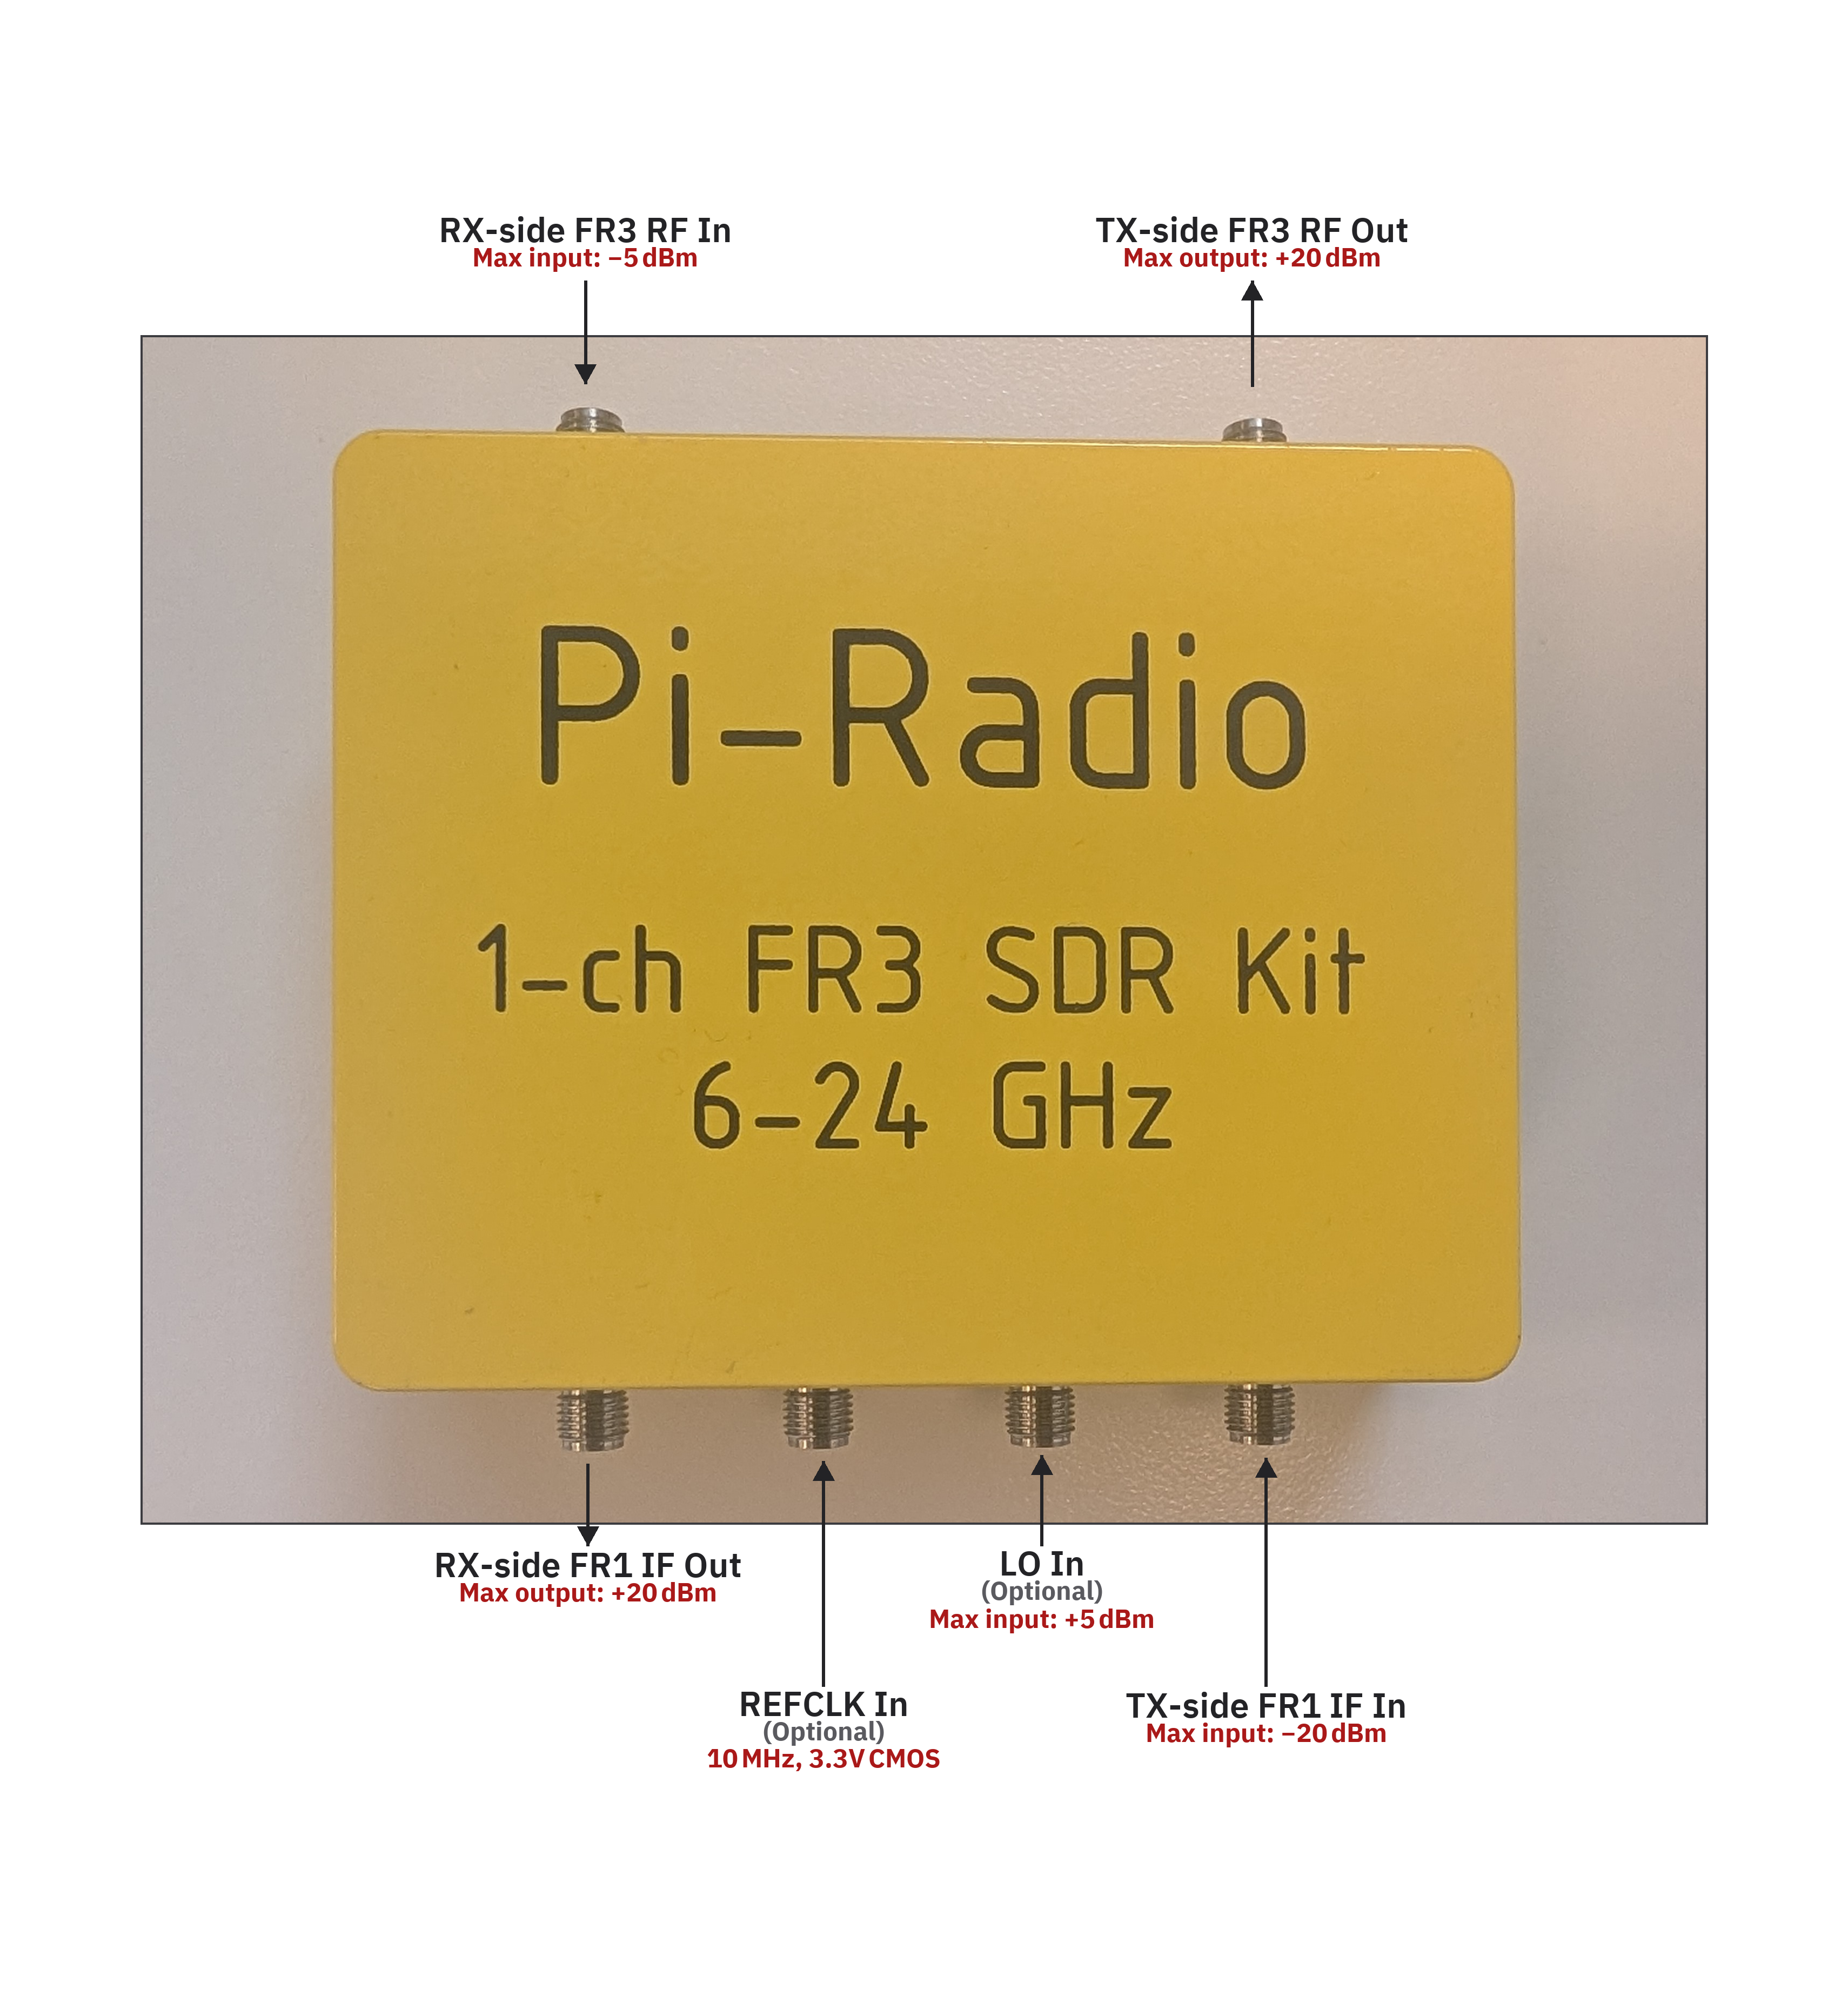
\includegraphics[width=0.56\linewidth]{images/hw_photo_labeled.png}
\vspace{-0.5em}
\captionof{figure}{The Pi-Radio FR3-1ch unit, all six SMA connectors labeled. Top row: the two FR3 (RF)
connectors. Bottom row: the two FR1 (IF) connectors and the two shared reference inputs (REFCLK, LO).}
\label{fig:hw-photo}
\end{center}
\vspace{-1.2em}

\subsection{Using the System}
\label{sec:hw-using-system}

\textbf{Why port, not rebuild.} The point of the Pi-Radio FR3-1ch unit is to let an FR1 experiment that already
works today --- a USRP, an RFSoC, a Wi-Fi chipset, a 5G modem, anything that already transmits and receives at
FR1 --- move up to FR3 without touching that system's own code at all. The existing FR1 radio keeps doing
exactly what it already does; the Pi-Radio box sits between it and the antenna and handles the up/down
conversion to and from FR3 transparently.

\textbf{TX side.} Take the transmit output of the existing FR1 system, pad it with an attenuator if its power
level calls for one, and feed it straight into the ``TX-side FR1 IF In'' connector (Figure~\ref{fig:hw-photo}).
The desired experiment --- the FR1 frequency, the target FR3 frequency, the signal bandwidth, and which sideband
to use --- is set either through the Pi-Radio GUI or directly over the USB-serial interface described in
Section~\ref{sec:hw-digital}; the unit works out the LO frequency and switch states that configuration implies
on its own. The up-converted result appears at the ``TX-side FR3 RF Out'' connector, ready to go to an antenna
or any other FR3 test setup.

\textbf{RX side.} The receive path is the mirror image of the TX path, and it is not configured separately: it
automatically takes on whatever FR1 frequency, FR3 frequency, bandwidth, and sideband the TX side was just told
to use. An FR3 signal arriving at the ``RX-side FR3 RF In'' connector comes back out as the corresponding FR1
signal at the ``RX-side FR1 IF Out'' connector, which feeds directly into the existing FR1 system's receive
input (again through an attenuator if needed).

\textbf{Phase coherence across units.} A single internal 10\,MHz TCXO and PLL/VCO (Section~\ref{sec:hw-clock-lo})
generates the one LO that both the TX and RX chains share, so a single unit's TX and RX are automatically phase
coherent with each other. Tiling several units together for multi-channel, phase-coherent operation is also
supported, with a choice of two approaches. The cheaper and simpler option distributes one common external
10\,MHz reference to every unit's ``REFCLK In'' connector through a clock buffer --- each unit still runs its
own LO, merely locked to a shared timebase. The other option distributes a single LO directly to every unit's
``LO In'' connector instead, generated by the Pi-Radio OctoLO (a phase-coherent 8-channel LO source built for
exactly this purpose), bypassing each unit's own synthesizer; this gives substantially lower phase noise
(Section~\ref{sec:phase-noise}), at the cost of needing the OctoLO itself. As a general rule of thumb, sharing one
LO keeps the units' phases more tightly aligned than sharing only the 10\,MHz reference, since each unit's own
synthesizer then no longer adds its own independent phase wander.

\textbf{Power and control.} The whole unit is powered from a single USB-C connector; the supply behind it must
be able to source 1.5\,A, since the unit draws 7.5\,W from 5\,V. If a computer's or laptop's own USB-C port
cannot source that much current directly, a powered USB-C hub in between works just as well. That same USB-C
connector also carries the
serial link used to configure everything described above --- the Pi-Radio GUI talks over this same serial
interface rather than some separate side channel, so anything the GUI can do is also reachable directly by a
script talking the same ASCII command set (Section~\ref{sec:hw-digital}).

\subsection{TX-side Up-conversion: FR1 $\to$ FR3}
\label{sec:hw-tx}

\textbf{Signal path.} An external FR1 signal (0.7--4.0\,GHz, up to 500\,MHz of instantaneous bandwidth) enters the unit's
``TX-side FR1 IF In'' connector (Figure~\ref{fig:hw-photo}) and passes through a fixed-gain amplifier (Analog
Devices ADL5545), then a 90$^\circ$ hybrid
coupler (Mini-Circuits QCH-392+) that splits it into two copies 90$^\circ$ apart in phase, FR1\_I and FR1\_Q.
These two lines pass through a DPDT switch (thru/swap) and then into the I and Q ports of a quadrature mixer
(MACOM MAMX-011075) together with the shared LO (Section~\ref{sec:hw-clock-lo}). A DC bias (I\_V, Q\_V),
produced by an on-board multi-channel DAC, is injected onto the same I/Q lines between the switch and the mixer specifically
to null the mixer's own LO-to-RF leakage (see Section~\ref{sec:lo-suppression}). After the mixer, the RF output
passes through a Mercury Systems AM3153 programmable bandpass filter, a fixed-gain LNA (HMC963), a fixed-gain final power amplifier
(Analog Devices ADL9006), and out through the ``TX-side FR3 RF Out'' connector. ``Fixed-gain'' means none of these
amplifier stages are software-adjustable --- the only thing under digital control on this path is the DPDT
switch state, the I/Q DC biases, and the AM3153 filter's selected sub-state.

\textbf{Upper vs.\ lower sideband.} The mixer is a full I/Q (quadrature) upconverter: with the DPDT switch in
``thru,'' the upper sideband dominates the RF output; in ``swap,'' the lower sideband dominates instead. This is
not merely a filter choice --- it changes which of the two possible LO frequencies the unit must tune to for a
given desired FR3 output, and whether the FR1 input's own internal spectral content comes out the same way
round or mirrored:
{\setlength{\topsep}{0.2em}\setlength{\partopsep}{0pt}\begin{itemize}\setlength{\itemsep}{0.3em}\setlength{\parskip}{0pt}
\item \textbf{Upper sideband (thru):} LO = FR3 $-$ FR1. The LO sits below FR3 (low-side). No spectral flip --- a
feature that sits at the \emph{high} end of the FR1 passband shows up at the \emph{high} end of FR3's occupied
band too.
\item \textbf{Lower sideband (swap):} LO = FR3 $+$ FR1. The LO sits above FR3 (high-side). The spectrum flips
--- a feature at the \emph{high} end of FR1 shows up at the \emph{low} end of FR3's occupied band, and vice
versa.
\end{itemize}}
Figure~\ref{fig:hw-tx-block} shows the full chain. Figure~\ref{fig:hw-tx-spectrum} shows the flip itself: the
input spectrum shown is deliberately asymmetric (steep on one edge, shallow on the other) so the mirroring is
visible at a glance in the lower-sideband case.

\noindent\begin{minipage}{\linewidth}
\centering
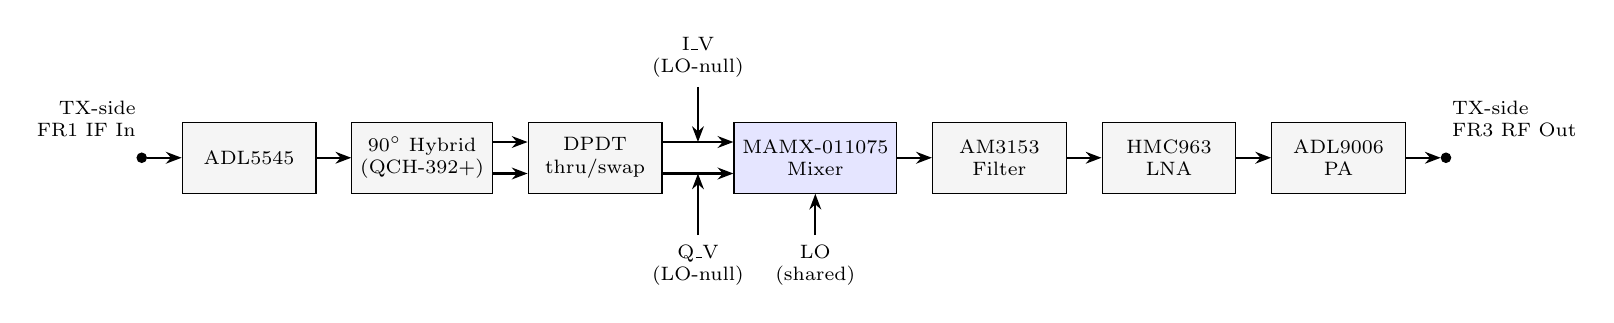
\begin{tikzpicture}[
  block/.style={draw, rectangle, minimum height=0.9cm, minimum width=1.7cm, align=center, font=\scriptsize,
                fill=gray!8, inner sep=3pt},
  mixblock/.style={block, fill=blue!10},
  conn/.style={draw, circle, minimum size=2pt, fill=black, inner sep=1.2pt},
  arr/.style={-{Stealth[length=2mm]}, thick},
  sidelabel/.style={font=\scriptsize, align=center},
  node distance=4.4mm  % 4.4 (not 5) so the outward connector labels keep the figure within the text width
]
\node[conn] (fr1in) {};
\node[sidelabel, anchor=south east, align=right] at ([yshift=1mm]fr1in.north east) {TX-side\\FR1 IF In};
\node[block, right=of fr1in] (amp1) {ADL5545};
\node[block, right=of amp1] (hyb) {90$^\circ$ Hybrid\\(QCH-392+)};
\node[block, right=of hyb] (dpdt) {DPDT\\thru/swap};
\node[mixblock, right=9mm of dpdt] (mix) {MAMX-011075\\Mixer};
\node[block, right=of mix] (filt) {AM3153\\Filter};
\node[block, right=of filt] (lna) {HMC963\\LNA};
\node[block, right=of lna] (pa) {ADL9006\\PA};
\node[conn, right=of pa] (fr3out) {};
\node[sidelabel, anchor=south west, align=left] at ([yshift=1mm]fr3out.north west) {TX-side\\FR3 RF Out};

\draw[arr] (fr1in) -- (amp1);
\draw[arr] (amp1) -- (hyb);
\draw[arr] ([yshift=2mm]hyb.east) -- ([yshift=2mm]dpdt.west);
\draw[arr] ([yshift=-2mm]hyb.east) -- ([yshift=-2mm]dpdt.west);
\draw[arr] ([yshift=2mm]dpdt.east) -- ([yshift=2mm]mix.west) coordinate[pos=0.5] (iline-mid);
\draw[arr] ([yshift=-2mm]dpdt.east) -- ([yshift=-2mm]mix.west) coordinate[pos=0.5] (qline-mid);
\draw[arr] (mix) -- (filt);
\draw[arr] (filt) -- (lna);
\draw[arr] (lna) -- (pa);
\draw[arr] (pa) -- (fr3out);

% LO and Q_V labels share one text baseline (anchor=base), so they sit exactly level; each arrow runs straight
% up from its label's top edge and its tip stops exactly on the target (the mixer's bottom edge / the Q line).
\coordinate (botbase) at ([yshift=-11mm]mix.south);
\node[sidelabel, anchor=base] (lo) at (mix |- botbase) {LO\\(shared)};
\draw[arr] (lo.north) -- (mix.south);
\node[sidelabel, above=7mm of iline-mid] (ibias) {I\_V\\(LO-null)};
\draw[arr] (ibias.south) -- (iline-mid);
\node[sidelabel, anchor=base] (qbias) at (qline-mid |- botbase) {Q\_V\\(LO-null)};
\draw[arr] (qbias.north) -- (qline-mid);
\end{tikzpicture}
\captionof{figure}{TX-side signal chain. Fixed-gain amplifiers and filters (grey) surround the quadrature
mixer (blue); the DPDT switch and the shared LO (Section~\ref{sec:hw-clock-lo}) together set which sideband and
which actual RF frequency come out.}
\label{fig:hw-tx-block}
\end{minipage}

\noindent\begin{minipage}{\linewidth}
\centering
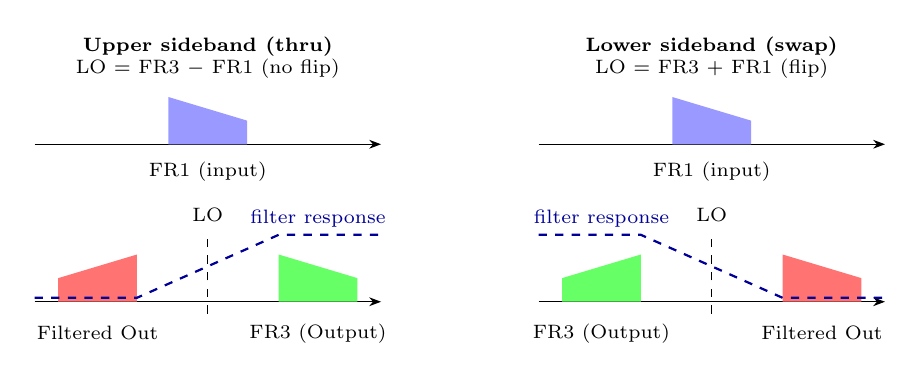
\begin{tikzpicture}[font=\scriptsize]
  % ---- Panel A: Upper sideband (thru), no flip ----
  \begin{scope}[xshift=0cm]
    \node[align=center] at (0,3.1) {\textbf{Upper sideband (thru)}\\LO = FR3 $-$ FR1 (no flip)};
    \draw[-{Stealth[length=1.5mm]}] (-2.2,2) -- (2.2,2);
    \fill[blue!40] (-0.5,2) -- (-0.5,2.6) -- (0.5,2.3) -- (0.5,2) -- cycle;
    \node at (0,1.65) {FR1 (input)};
    \draw[-{Stealth[length=1.5mm]}] (-2.2,0) -- (2.2,0);
    \draw[dashed] (0,-0.15) -- (0,0.9);
    \node at (0,1.1) {LO};
    \fill[green!60] (0.9,0) -- (0.9,0.6) -- (1.9,0.3) -- (1.9,0) -- cycle;
    \node at (1.4,-0.4) {FR3 (Output)};
    \fill[red!55] (-1.9,0) -- (-1.9,0.3) -- (-0.9,0.6) -- (-0.9,0) -- cycle;
    \node at (-1.4,-0.4) {Filtered Out};
    \draw[blue!60!black, dashed, thick] (-2.2,0.05) -- (-0.9,0.05) -- (0.9,0.85) -- (2.2,0.85);
    \node[blue!60!black] at (1.4,1.05) {filter response};
  \end{scope}
  % ---- Panel B: Lower sideband (swap), flip ----
  \begin{scope}[xshift=6.4cm]
    \node[align=center] at (0,3.1) {\textbf{Lower sideband (swap)}\\LO = FR3 $+$ FR1 (flip)};
    \draw[-{Stealth[length=1.5mm]}] (-2.2,2) -- (2.2,2);
    \fill[blue!40] (-0.5,2) -- (-0.5,2.6) -- (0.5,2.3) -- (0.5,2) -- cycle;
    \node at (0,1.65) {FR1 (input)};
    \draw[-{Stealth[length=1.5mm]}] (-2.2,0) -- (2.2,0);
    \draw[dashed] (0,-0.15) -- (0,0.9);
    \node at (0,1.1) {LO};
    \fill[green!60] (-1.9,0) -- (-1.9,0.3) -- (-0.9,0.6) -- (-0.9,0) -- cycle;
    \node at (-1.4,-0.4) {FR3 (Output)};
    \fill[red!55] (0.9,0) -- (0.9,0.6) -- (1.9,0.3) -- (1.9,0) -- cycle;
    \node at (1.4,-0.4) {Filtered Out};
    \draw[blue!60!black, dashed, thick] (-2.2,0.85) -- (-0.9,0.85) -- (0.9,0.05) -- (2.2,0.05);
    \node[blue!60!black] at (-1.4,1.05) {filter response};
  \end{scope}
\end{tikzpicture}
\captionof{figure}{The same asymmetric FR1 input (blue, taller edge on the left in both panels) up-converted
two ways, each producing both a desired sideband (green) and an unwanted image sideband (red) on the mixer's
output. The dashed blue curve is a stand-in for the AM3153 filter's response: low over the image sideband
(rejected) and high over the desired one (passed through). Upper sideband reproduces the input shape unchanged at
FR3 --- the tall edge is still on the left. Lower sideband mirrors it --- the tall edge moves to the right ---
because the LO has moved from below FR3 to above it.}
\label{fig:hw-tx-spectrum}
\end{minipage}

\subsection{RX-side down-conversion: FR3 $\to$ FR1}
\label{sec:hw-rx}

\textbf{Signal path.} An external RF signal enters the ``RX-side FR3 RF In'' connector (Figure~\ref{fig:hw-photo})
and is amplified by a fixed-gain LNA (HMC963). It then passes through a Mercury
Systems AM3153 programmable bandpass filter before
reaching a quadrature mixer (MACOM MAMX-011075). Unlike the TX side, the RX chain is \emph{not} used as a full I/Q receiver: the mixer's I and Q outputs
carry the same information rotated 90$^\circ$ apart, but only the I output is kept as the board's IF signal ---
the Q output is simply terminated into 50$\,\Omega$ and discarded. The kept output passes through a fixed
4500\,MHz low-pass filter (removing the mixer's harmless RF+LO sum product, which lands tens of GHz away) and
then two cascaded IF amplifier stages (both Analog Devices ADL5545, the same part used as the TX chain's first
FR1 amplifier), before leaving through the ``RX-side FR1 IF Out'' connector.

\textbf{Why there's still image rejection, without I/Q.} Because only I is kept, the RX side has no I/Q-based
image-reject mechanism and no independent sideband-selection switch the way TX does. Image rejection instead
comes entirely from the AM3153 filter sitting \emph{before} the mixer: it attenuates the unwanted image
frequency (the other real RF frequency, on the opposite side of the LO from the one actually wanted) before it
ever reaches the mixer --- the classic filter-based (as opposed to I/Q-based) image-rejection technique,
covered in depth in Section~\ref{sec:rx-image-rejection}.

\textbf{Low-side vs.\ high-side LO.} Because the RX mixer is a plain real mixer with no I/Q sideband selection,
which physical RF frequency ends up at a given IF output --- and whether the IF spectrum comes out flipped or
not --- is decided entirely by which side of FR3 the LO sits on:
{\setlength{\topsep}{0.2em}\setlength{\partopsep}{0pt}\begin{itemize}\setlength{\itemsep}{0.3em}\setlength{\parskip}{0pt}
\item \textbf{Low-side LO:} LO $<$ FR3, so IF = FR3 $-$ LO. No spectral flip --- IF increases as FR3 increases.
\item \textbf{High-side LO:} LO $>$ FR3, so IF = LO $-$ FR3. The spectrum flips --- IF \emph{decreases} as FR3
increases.
\end{itemize}}
Unlike TX, this is not a switch the RX side can set independently: TX and RX share one physical LO
(Section~\ref{sec:hw-clock-lo}), so TX's sideband choice and RX's low/high-side state are locked together ---
TX upper sideband forces RX low-side (no flip) at the same instant, and TX lower sideband forces RX high-side
(flip) at the same instant. Figure~\ref{fig:hw-rx-block}
shows the full chain, and Figure~\ref{fig:hw-rx-spectrum} shows the resulting flip, using the same asymmetric-spectrum
convention as Figure~\ref{fig:hw-tx-spectrum}.

\noindent\begin{minipage}{\linewidth}
\centering
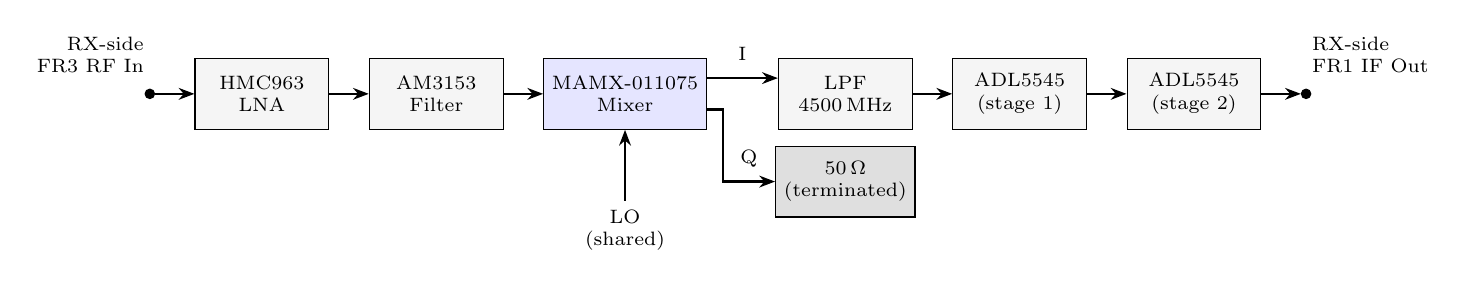
\begin{tikzpicture}[
  block/.style={draw, rectangle, minimum height=0.9cm, minimum width=1.7cm, align=center, font=\scriptsize,
                fill=gray!8, inner sep=3pt},
  mixblock/.style={block, fill=blue!10},
  term/.style={block, fill=gray!25, minimum width=1.3cm},
  conn/.style={draw, circle, minimum size=2pt, fill=black, inner sep=1.2pt},
  arr/.style={-{Stealth[length=2mm]}, thick},
  sidelabel/.style={font=\scriptsize, align=center},
  node distance=5mm
]
\node[conn] (fr3in) {};
\node[sidelabel, anchor=south east, align=right] at ([yshift=1mm]fr3in.north east) {RX-side\\FR3 RF In};
\node[block, right=of fr3in] (lna) {HMC963\\LNA};
\node[block, right=of lna] (filt) {AM3153\\Filter};
\node[mixblock, right=of filt] (mix) {MAMX-011075\\Mixer};
\node[block, right=9mm of mix] (lpf) {LPF\\4500\,MHz};
\node[block, right=of lpf] (amp1) {ADL5545\\(stage 1)};
\node[block, right=of amp1] (amp2) {ADL5545\\(stage 2)};
\node[conn, right=of amp2] (fr1out) {};
\node[sidelabel, anchor=south west, align=left] at ([yshift=1mm]fr1out.north west) {RX-side\\FR1 IF Out};
\node[term, below=2mm of lpf] (qterm) {50\,$\Omega$\\(terminated)};

\draw[arr] (fr3in) -- (lna);
\draw[arr] (lna) -- (filt);
\draw[arr] (filt) -- (mix);
\draw[arr] ([yshift=2mm]mix.east) -- ([yshift=2mm]lpf.west) coordinate[pos=0.5] (iline-mid);
\node[sidelabel, above=1mm of iline-mid] {I};
\draw[arr] ([yshift=-2mm]mix.east) -- ++(2mm,0) |- (qterm.west)
  node[sidelabel, pos=0.75, above=0.5mm] {Q};  % pos 0.75 = middle of the horizontal run into the termination
\draw[arr] (lpf) -- (amp1);
\draw[arr] (amp1) -- (amp2);
\draw[arr] (amp2) -- (fr1out);

\node[sidelabel, below=9mm of mix] (lo) {LO\\(shared)};
\draw[arr] (lo) -- (mix.south);
\end{tikzpicture}
\captionof{figure}{RX-side signal chain. The same mixer part as TX (blue) is used, but only its I output is
kept --- Q is simply terminated. The shared LO (Section~\ref{sec:hw-clock-lo}) feeds this mixer too. Image
rejection comes entirely from the AM3153 filter positioned \emph{before} the mixer
(Section~\ref{sec:rx-image-rejection}), not from any I/Q cancellation after it.}
\label{fig:hw-rx-block}
\end{minipage}

\noindent\begin{minipage}{\linewidth}
\centering
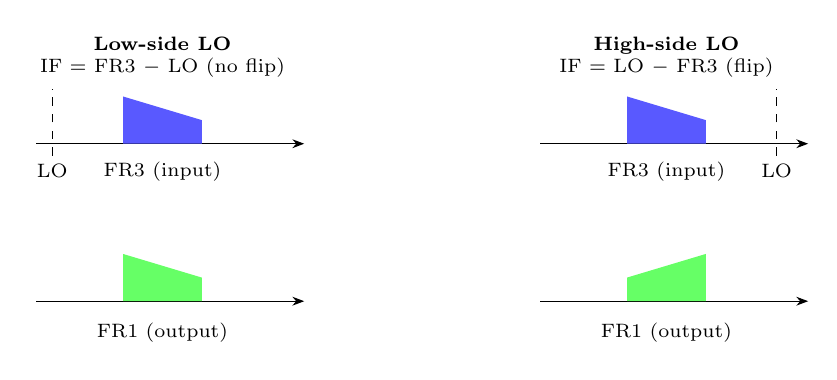
\begin{tikzpicture}[font=\scriptsize]
  % ---- Panel A: Low-side LO, no flip ----
  \begin{scope}[xshift=0cm]
    \node[align=center] at (0,3.1) {\textbf{Low-side LO}\\IF = FR3 $-$ LO (no flip)};
    \draw[-{Stealth[length=1.5mm]}] (-1.6,2) -- (1.8,2);
    \fill[blue!65] (-0.5,2) -- (-0.5,2.6) -- (0.5,2.3) -- (0.5,2) -- cycle;
    \node at (0,1.65) {FR3 (input)};
    % the LO lives on the FR3 (input) axis: below the signal for low-side
    \draw[dashed] (-1.4,1.85) -- (-1.4,2.7);
    \node at (-1.4,1.65) {LO};
    \draw[-{Stealth[length=1.5mm]}] (-1.6,0) -- (1.8,0);
    \fill[green!60] (-0.5,0) -- (-0.5,0.6) -- (0.5,0.3) -- (0.5,0) -- cycle;
    \node at (0,-0.4) {FR1 (output)};
  \end{scope}
  % ---- Panel B: High-side LO, flip ----
  \begin{scope}[xshift=6.4cm]
    \node[align=center] at (0,3.1) {\textbf{High-side LO}\\IF = LO $-$ FR3 (flip)};
    \draw[-{Stealth[length=1.5mm]}] (-1.6,2) -- (1.8,2);
    \fill[blue!65] (-0.5,2) -- (-0.5,2.6) -- (0.5,2.3) -- (0.5,2) -- cycle;
    \node at (0,1.65) {FR3 (input)};
    % ...and above the signal for high-side
    \draw[dashed] (1.4,1.85) -- (1.4,2.7);
    \node at (1.4,1.65) {LO};
    \draw[-{Stealth[length=1.5mm]}] (-1.6,0) -- (1.8,0);
    \fill[green!60] (-0.5,0) -- (-0.5,0.3) -- (0.5,0.6) -- (0.5,0) -- cycle;
    \node at (0,-0.4) {FR1 (output)};
  \end{scope}
\end{tikzpicture}
\captionof{figure}{The same asymmetric FR3 input (blue, tall edge on the left in both panels) down-converted
two ways to the FR1 output (green). Low-side LO reproduces that shape unchanged at FR1. High-side LO mirrors it,
exactly as the lower sideband did on the TX side (Figure~\ref{fig:hw-tx-spectrum}) --- but here it is a forced
consequence of the shared LO's position, not a choice RX itself makes.}
\label{fig:hw-rx-spectrum}
\end{minipage}

\subsection{Clocking and LO}
\label{sec:hw-clock-lo}

\textbf{One synthesizer, shared by both chains.} A single LO signal, generated by one LMX2820 fractional-N
synthesizer, feeds both the TX mixer and the RX mixer simultaneously --- there is no separate TX LO and RX LO.
This is exactly why TX's sideband state and RX's low/high-side state are consistent with each other (see above):
both are just different ways of comparing the same shared LO frequency against the same FR3. The LMX2820 tunes
anywhere from 6\,GHz to 22.6\,GHz; the controlling STM32 computes all 123 of its PLL registers directly from a
requested frequency in Hz and writes them over SPI, using a fractional-N denominator large enough to hit any
requested integer Hz exactly --- there is no rounding to a coarse channel grid. Output drive level is
software-settable (0--7); by default the firmware sets it from the LO frequency on every tune (0 up to 13\,GHz, 2 from
above 13 to below 20\,GHz, 4 from 20\,GHz up), and the chip can be fully muted (powered down) or read back for lock status and die
temperature.

\textbf{Internal vs.\ external, for both the clock and the LO.} Two independent switches exist here, easy to
conflate but serving different purposes. The \emph{clock} switch selects what reference the LMX2820's own PLL
locks to: an onboard reference (Internal) or a signal brought in on the ``REFCLK In'' connector
(Figure~\ref{fig:hw-photo}, External) --- this is the timebase the synthesizer measures its output frequency
against. The \emph{LO} switch is a separate, higher-level choice: Internal routes the LMX2820's own output into
the shared LO distribution feeding both mixers, while External bypasses the LMX2820 entirely and routes an
externally-supplied LO signal (via the ``LO In'' connector)
to both mixers instead. Selecting External LO automatically mutes the internal LMX2820 and switches off the internal 10\,MHz
reference clock (and switching back to Internal turns the reference clock back on, then un-mutes and re-tunes
the LMX2820), so the internal and external LO paths can never both drive the mixers at once. Figure~\ref{fig:hw-clock-lo-block} shows both switches and how the shared LO reaches both chains.

\noindent\begin{minipage}{\linewidth}
\centering
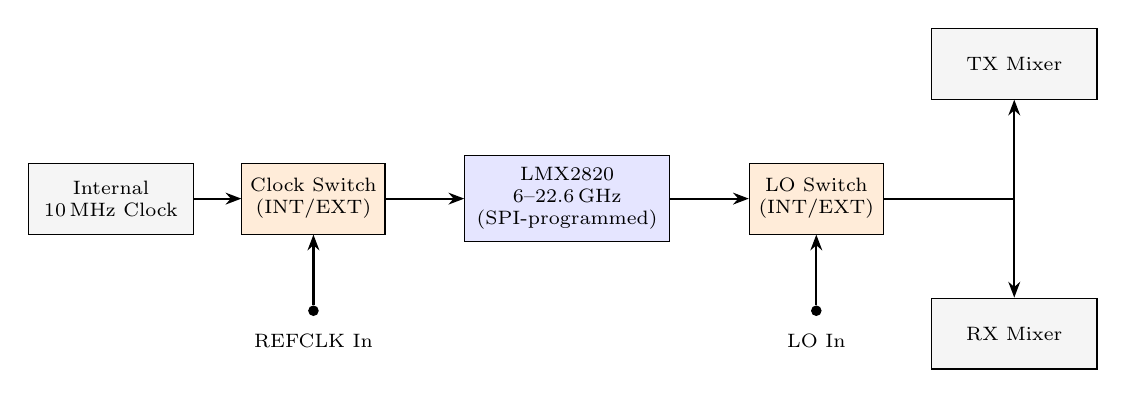
\begin{tikzpicture}[
  block/.style={draw, rectangle, minimum height=0.9cm, minimum width=2.1cm, align=center, font=\scriptsize,
                fill=gray!8, inner sep=3pt},
  swblock/.style={block, fill=orange!15, minimum width=1.7cm},
  synthblock/.style={block, fill=blue!10, minimum width=2.6cm, minimum height=1.1cm},
  conn/.style={draw, circle, minimum size=2pt, fill=black, inner sep=1.2pt},
  arr/.style={-{Stealth[length=2mm]}, thick},
  sidelabel/.style={font=\scriptsize, align=center},
  node distance=6mm
]
\node[block] (ref) {Internal\\10\,MHz Clock};
\node[swblock, right=of ref] (clksw) {Clock Switch\\(INT/EXT)};
\node[conn, below=9mm of clksw] (extclk) {};
% both external-input dots share one height, and both labels one text baseline (anchor=base: "Clock" has taller
% ascenders than "LO", so aligning the label boxes' tops would leave the text 0.2pt apart)
\coordinate (extrow) at (extclk.center);
\coordinate (extlabelbase) at ([yshift=-4mm]extclk.south);
\node[sidelabel, anchor=base] at (extclk |- extlabelbase) {REFCLK In};
\draw[arr] (ref) -- (clksw);
\draw[arr] (extclk) -- (clksw.south);
\node[synthblock, right=10mm of clksw] (lmx) {LMX2820\\6--22.6\,GHz\\(SPI-programmed)};
\draw[arr] (clksw) -- (lmx);
\node[swblock, right=10mm of lmx] (losw) {LO Switch\\(INT/EXT)};
\draw[arr] (lmx) -- (losw);
\node[conn] (extlo) at (losw |- extrow) {};
\node[sidelabel, anchor=base] at (extlo |- extlabelbase) {LO In};
\draw[arr] (extlo) -- (losw.south);  % straight: a |- path here has a zero-length last leg, which pushes the line into the box
\node[block, above right=8mm and 6mm of losw] (txmix) {TX Mixer};
\node[block, below right=8mm and 6mm of losw] (rxmix) {RX Mixer};
\draw[arr] (losw) -| (txmix);
\draw[arr] (losw) -| (rxmix);
\end{tikzpicture}
\captionof{figure}{Clock and LO distribution. The clock switch picks what reference the LMX2820 locks to; the
LO switch separately picks whether the LMX2820's own output, or an external LO altogether, feeds both mixers.
Both switches default to Internal.}
\label{fig:hw-clock-lo-block}
\end{minipage}

\subsection{Digital and Control}
\label{sec:hw-digital}

\textbf{Microcontroller and firmware.} An STM32H573VITx (Arm Cortex-M33) runs the unit's firmware on top of
Azure RTOS ThreadX, with ST's USBX middleware implementing a USB CDC-ACM virtual serial port --- this is the
single interface the GUI and every measurement script in this project talk to. The protocol is a plain
line-based ASCII command/response scheme (e.g.\ \texttt{LMX TUNE 12000000000} $\to$ \texttt{OK}, \texttt{GET
TXFILTER} $\to$ \texttt{0x3C}): every command is echoed back, followed by one response line. The firmware has no
concept of ``FR1''/``FR3''/``sideband'' at all --- that translation is entirely a host-side computation (done by
the GUI's Configuration Helper, or by a measurement script); the firmware only ever receives a plain tune
frequency, a plain filter byte, a plain switch state. Two things it does set by itself: the LO drive level, from the LO
frequency, and the TX LO-null bias voltages, from the unit's own calibration stored in its flash
(Section~\ref{sec:lo-suppression}); both can be switched to manual (Appendix~\ref{sec:commands}).

\textbf{Peripheral buses.} The STM32 talks to the LMX2820 synthesizer and to an LTC2668 multi-channel DAC (the
source of the TX-side I\_V/Q\_V bias voltages) over a shared SPI bus, and drives the Clock-source, LO-source,
and IQ-swap switches, plus the TX and RX AM3153 filter control lines, directly over GPIO.

\textbf{Persistence.} Every one of these settings --- LMX2820 frequency/power/mute state, I\_V/Q\_V bias, clock
and LO source, IQ swap, and both filter selections --- is mirrored into the STM32H5's EDATA flash region, so the
unit powers back up into whatever state it was last left in, with no host required. A \texttt{SET PERSIST
OFF}/\texttt{ON} pair lets a long measurement sweep suspend flash writes for its duration (so thousands of
setting changes in a sweep don't wear the flash) and then commit the unit's final state once, at the end. A
separate, factory-programmed board serial number (distinct from the COM port enumeration, which can change)
lets the GUI and measurement scripts identify a specific physical unit regardless of which USB port it is
plugged into. Figure~\ref{fig:hw-digital-block} shows how these pieces fit together.

\noindent\begin{minipage}{\linewidth}
\centering
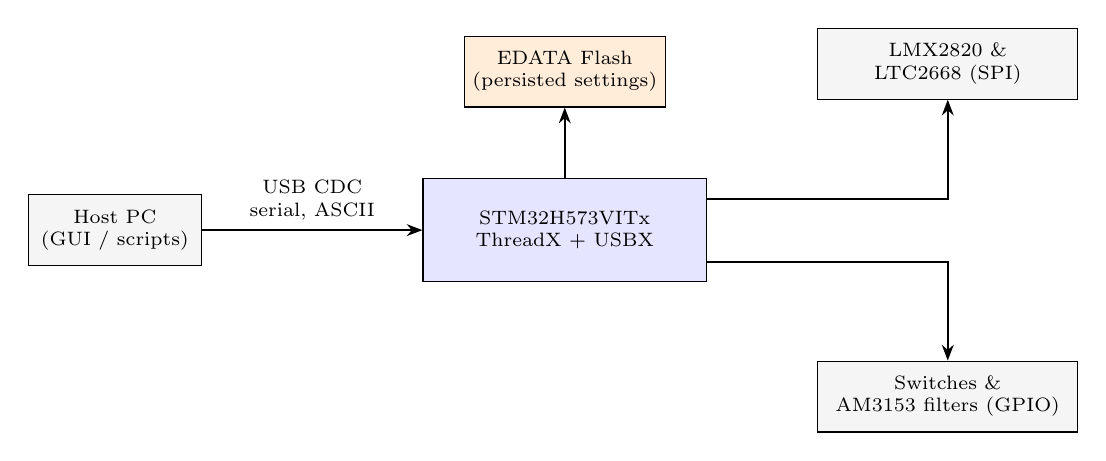
\begin{tikzpicture}[
  block/.style={draw, rectangle, minimum height=0.9cm, minimum width=2.2cm, align=center, font=\scriptsize,
                fill=gray!8, inner sep=3pt},
  mcublock/.style={block, fill=blue!10, minimum width=3.6cm, minimum height=1.3cm},
  flashblock/.style={block, fill=orange!15},
  arr/.style={-{Stealth[length=2mm]}, thick},
  node distance=9mm
]
\node[block] (host) {Host PC\\(GUI / scripts)};
\node[mcublock, right=28mm of host] (mcu) {STM32H573VITx\\ThreadX + USBX};
\draw[arr] (host) -- node[above, font=\scriptsize, align=center]{USB CDC\\serial, ASCII} (mcu);
\node[flashblock, above=9mm of mcu] (flash) {EDATA Flash\\(persisted settings)};
\draw[arr] (mcu) -- (flash);
\node[block, above right=10mm and 14mm of mcu, minimum width=3.3cm] (spi) {LMX2820 \&\\LTC2668 (SPI)};
\node[block, below right=10mm and 14mm of mcu, minimum width=3.3cm] (gpio) {Switches \&\\AM3153 filters (GPIO)};
\draw[arr] ([yshift=4mm]mcu.east) -| (spi.south);
\draw[arr] ([yshift=-4mm]mcu.east) -| (gpio.north);
\end{tikzpicture}
\captionof{figure}{Digital control architecture. The STM32 is the sole point of contact for the host; it never
exposes FR1/FR3/sideband concepts, only raw frequencies, filter bytes, and switch states.}
\label{fig:hw-digital-block}
\end{minipage}

\clearpage
\flushbottom

\clearpage
\section{TX-side Conversion Gain --- Upper Sideband (No Spectral Flip)}
\label{sec:tx-gain-upper}

\textbf{What is conversion gain?} The TX side takes a signal in at FR1 and sends it out at a much higher FR3
frequency, amplifying it along the way. Conversion gain measures that amplification across the change of
frequency. Feed a signal into the ``TX-side FR1 IF In'' connector at, say, −40\,dBm, and measure the signal that comes out of the ``TX-side FR3 RF Out'' connector at its new frequency, say +5\,dBm. The conversion gain is simply the difference:
+5 − (−40) = 45\,dB. Because both powers are in dBm, subtracting them gives the conversion gain in dB directly.

\textbf{What's plotted.} Each of the first seven figures holds FR1 fixed at one center value (1.0 up to the
unit's 4.0\,GHz maximum, in 0.5\,GHz steps) and plots conversion gain against the full measured FR3 range for
that input.\footnote{Every point on both traces is a real measurement, never a simulation or an interpolation
between sparse samples: the FieldFox's built-in tracking generator drives FR1 while the FieldFox's own
receiver tracks the corresponding FR3 output in lock-step, at a calibrated −40\,dBm input level.} Grey is the
raw amplifier-and-mixer chain with the AM3153 filter bypassed; blue is the filter engaged. Both traces plot the
\emph{average} conversion gain across each point's own real swept window, nominally 500\,MHz wide (the same for
every point on every panel) --- mean linear power, converted back to dB, not a single CW tone: what a real
wideband signal occupying that window would experience. The gap between the two traces, at any point, is
exactly how much the filter costs in insertion loss there.

\textbf{Measurement conditions.} \lmxDriveRule{} (set from the LO frequency), with the LO leakage suppressed by the unit's stored LO-null calibration (Section~\ref{sec:lo-suppression}), exactly as in normal use. The unit was measured hot, as the worst case: no fan, LMX2820 die at \condGainMinC--\condGainMaxC\textdegree C. A cooler unit will typically do somewhat better.

\textbf{How the filter is chosen.} The blue trace's filter is re-picked fresh at every single plotted point,
using a two-step rule: first find whichever of the 48 candidate configurations (3 bands × 16 sub-states)
passes the most desired-sideband energy on its own, ignoring the image; then, restricted to candidates within
3\,dB of that best desired power, choose whichever rejects the image the most. Consecutive points that land on
the same filter form a \emph{region}; the dashed vertical lines on each panel mark every boundary between
regions, and the blue hex code running up from the x-axis inside each region (e.g.\ \texttt{0x3F}) is the
actual \texttt{filter\_bits} value used for every point in it --- so the exact filter behind any measurement is
always readable directly off the figure.

\textbf{Window width.} Every point averages over its own real swept window, and that window is always exactly
500\,MHz wide: a fixed filter setting's measured response across that full window is exactly what a real
wideband signal at that setting would experience.\footnote{The one exception worth noting is Figure
\ref{fig:1-7} (FR1 = 4.0\,GHz): its window is 3.75--4.25\,GHz at every point, and 250\,MHz of that exceeds the
unit's 0.7--4.0\,GHz IF design spec --- a real, measured operating point, called out directly on that panel
and outlined in red on the two heatmaps (Figures \ref{fig:1-8} and \ref{fig:1-9}).} Those two heatmaps repeat
the bypassed and optimal data across the full measured (FR1, FR3) grid, for a single-glance view instead of the seven separate slices above. FR3 values above the unit's rated 24\,GHz are boxed in red on both heatmaps
too: measured and shown, but out of design spec.

\figpair{images/sec1_fig1.pdf}{FR1 = 1.0\,GHz.}{fig:1-1}%
        {images/sec1_fig2.pdf}{FR1 = 1.5\,GHz.}{fig:1-2}
\figpair{images/sec1_fig3.pdf}{FR1 = 2.0\,GHz.}{fig:1-3}%
        {images/sec1_fig4.pdf}{FR1 = 2.5\,GHz.}{fig:1-4}
\figpair{images/sec1_fig5.pdf}{FR1 = 3.0\,GHz.}{fig:1-5}%
        {images/sec1_fig6.pdf}{FR1 = 3.5\,GHz.}{fig:1-6}
\figonesmall{images/sec1_fig7.pdf}{FR1 = 4.0\,GHz. 250\,MHz of this window falls outside the unit's IF design spec (shown in red).}{fig:1-7}
\figrow{images/sec1_fig8.pdf}{Conversion gain, upper sideband: full measured (FR1, FR3) grid, filter bypassed.
Zoom in to read each cell's exact values, printed as (FR1, FR3, conversion gain), with FR1 and FR3 in GHz and
the conversion gain in dB.}{fig:1-8}
\figrow{images/sec1_fig9.pdf}{Conversion gain, upper sideband: full measured (FR1, FR3) grid, optimal filter.
Zoom in to read each cell's exact values, printed as (FR1, FR3, conversion gain), with FR1 and FR3 in GHz and
the conversion gain in dB.}{fig:1-9}

\clearpage
\section{TX-side Conversion Gain --- Lower Sideband (Spectral Flip)}
\label{sec:tx-gain-lower}

\textbf{What is conversion gain?} Exactly as in Section~\ref{sec:tx-gain-upper}: the power of the signal coming out of the ``TX-side FR3 RF Out'' connector, minus the power of the signal fed into the ``TX-side FR1 IF In'' connector, both in dBm, gives
the conversion gain in dB. Only the sideband changes here, now the lower one instead of the upper.

\textbf{What's plotted.} Identical methodology to Section~\ref{sec:tx-gain-upper}, with the unit tuned to the
lower sideband instead of the upper: each of the first seven figures holds FR1 fixed at one center value (1.0
up to the unit's 4.0\,GHz maximum, in 0.5\,GHz steps) and plots conversion gain against the full measured FR3
range for that input.\footnote{Every point on both traces is a real measurement, never a simulation or an
interpolation between sparse samples: the FieldFox's built-in tracking generator drives FR1 while the
FieldFox's own receiver tracks the corresponding FR3 output in lock-step, at a calibrated −40\,dBm input
level.} Grey is the raw amplifier-and-mixer chain with the AM3153 filter bypassed; blue is the filter engaged.
Both traces plot the \emph{average} conversion gain across each point's own real swept window, nominally
500\,MHz wide (the same for every point on every panel) --- mean linear power, converted back to dB, not a
single CW tone: what a real wideband signal occupying that window would experience. The gap between the two
traces, at any point, is exactly how much the filter costs in insertion loss there, same as in
Section~\ref{sec:tx-gain-upper}.

\textbf{Measurement conditions.} \lmxDriveRule{} (set from the LO frequency), with the LO leakage suppressed by the unit's stored LO-null calibration (Section~\ref{sec:lo-suppression}), exactly as in normal use. The unit was measured hot, as the worst case: no fan, LMX2820 die at \condGainMinC--\condGainMaxC\textdegree C. A cooler unit will typically do somewhat better.

\textbf{How the filter is chosen.} The same two-step rule as Section~\ref{sec:tx-gain-upper}: first find
whichever of the 48 candidate configurations (3 bands × 16 sub-states) passes the most desired-sideband
energy on its own, ignoring the image; then, restricted to candidates within 3\,dB of that best desired power,
choose whichever rejects the image the most. Consecutive points that land on the same filter form a
\emph{region}; the dashed vertical lines on each panel mark every boundary between regions, and the blue hex
code running up from the x-axis inside each region (e.g.\ \texttt{0x30}) is the actual \texttt{filter\_bits}
value used for every point in it --- so, just as in Section~\ref{sec:tx-gain-upper}, the exact filter behind
any measurement on these panels is always readable directly off the figure, with no need to consult a separate
table.

\textbf{Window width.} Every point's window is exactly 500\,MHz wide, the same fixed window used throughout
Section~\ref{sec:tx-gain-upper}: a fixed filter setting's measured response across that full window is exactly
what a real wideband signal at that setting would experience.\footnote{As in Section~\ref{sec:tx-gain-upper},
Figure \ref{fig:2-7} (FR1 = 4.0\,GHz) is the one exception: its window is 3.75--4.25\,GHz, and 250\,MHz of that
exceeds the unit's 0.7--4.0\,GHz IF design spec --- called out directly on that panel and outlined in red on
Figures \ref{fig:2-8} and \ref{fig:2-9}.} For the lower sideband, the masked (invalid-LO) region of the heatmaps
sits at the opposite end of the FR3 axis from the upper sideband, since LO = FR3 + FR1 here rather than
FR3 − FR1. Those two heatmaps repeat the bypassed and optimal data across the full measured (FR1, FR3) grid,
for a single-glance view instead of the seven separate slices above, exactly as in Section~\ref{sec:tx-gain-upper}.

\figpair{images/sec2_fig1.pdf}{FR1 = 1.0\,GHz.}{fig:2-1}%
        {images/sec2_fig2.pdf}{FR1 = 1.5\,GHz.}{fig:2-2}
\figpair{images/sec2_fig3.pdf}{FR1 = 2.0\,GHz.}{fig:2-3}%
        {images/sec2_fig4.pdf}{FR1 = 2.5\,GHz.}{fig:2-4}
\figpair{images/sec2_fig5.pdf}{FR1 = 3.0\,GHz.}{fig:2-5}%
        {images/sec2_fig6.pdf}{FR1 = 3.5\,GHz.}{fig:2-6}

\figonesmall{images/sec2_fig7.pdf}{FR1 = 4.0\,GHz. 250\,MHz of this window falls outside the unit's IF design spec (shown in red).}{fig:2-7}
\figrow{images/sec2_fig8.pdf}{Conversion gain, lower sideband: full measured (FR1, FR3) grid, filter bypassed.
Zoom in to read each cell's exact values, printed as (FR1, FR3, conversion gain), with FR1 and FR3 in GHz and
the conversion gain in dB.}{fig:2-8}
\figrow{images/sec2_fig9.pdf}{Conversion gain, lower sideband: full measured (FR1, FR3) grid, optimal filter.
Zoom in to read each cell's exact values, printed as (FR1, FR3, conversion gain), with FR1 and FR3 in GHz and
the conversion gain in dB.}{fig:2-9}

\clearpage
\section{TX-side Gain Flatness}
\label{sec:tx-flatness}
\raggedbottom% no stretched gaps between text and figures (as in the NF section)
% Generated by FR3_Characterization/plot_datasheet_flatness.py -- do not edit by hand.
\newcommand{\flatTxUpperBypassMedian}{1.55}
\newcommand{\flatTxUpperBypassPninety}{2.79}
\newcommand{\flatTxUpperBypassMin}{0.20}
\newcommand{\flatTxUpperBypassMax}{3.63}
\newcommand{\flatTxUpperOptimalMedian}{1.51}
\newcommand{\flatTxUpperOptimalPninety}{2.55}
\newcommand{\flatTxUpperOptimalMin}{0.17}
\newcommand{\flatTxUpperOptimalMax}{3.29}
\newcommand{\flatTxLowerBypassMedian}{1.21}
\newcommand{\flatTxLowerBypassPninety}{2.22}
\newcommand{\flatTxLowerBypassMin}{0.19}
\newcommand{\flatTxLowerBypassMax}{2.74}
\newcommand{\flatTxLowerOptimalMedian}{1.26}
\newcommand{\flatTxLowerOptimalPninety}{2.19}
\newcommand{\flatTxLowerOptimalMin}{0.16}
\newcommand{\flatTxLowerOptimalMax}{3.07}
\newcommand{\flatRxLowBypassMedian}{1.03}
\newcommand{\flatRxLowBypassPninety}{1.76}
\newcommand{\flatRxLowBypassMin}{0.46}
\newcommand{\flatRxLowBypassMax}{2.63}
\newcommand{\flatRxLowOptimalMedian}{0.95}
\newcommand{\flatRxLowOptimalPninety}{1.48}
\newcommand{\flatRxLowOptimalMin}{0.39}
\newcommand{\flatRxLowOptimalMax}{2.24}
\newcommand{\flatRxHighBypassMedian}{0.95}
\newcommand{\flatRxHighBypassPninety}{1.74}
\newcommand{\flatRxHighBypassMin}{0.37}
\newcommand{\flatRxHighBypassMax}{2.89}
\newcommand{\flatRxHighOptimalMedian}{0.90}
\newcommand{\flatRxHighOptimalPninety}{1.81}
\newcommand{\flatRxHighOptimalMin}{0.38}
\newcommand{\flatRxHighOptimalMax}{3.19}
\newcommand{\flatTxPpRatio}{3.3}
\newcommand{\flatTxPpRatioLow}{2.8}
\newcommand{\flatTxPpRatioHigh}{4.1}
\newcommand{\flatRxPpRatio}{4.5}
\newcommand{\flatRxPpRatioLow}{3.7}
\newcommand{\flatRxPpRatioHigh}{5.2}


\textbf{What is gain flatness?} Sections~\ref{sec:tx-gain-upper} and \ref{sec:tx-gain-lower} give the
\emph{average} conversion gain across a 500\,MHz window. A wideband signal also cares how much the gain varies
\emph{within} that window: if one part of the channel is amplified more than another, the signal comes out with a
tilted or rippled spectrum, and the pieces of it that sit at different frequencies (for example the sub-carriers of
an OFDM signal) arrive at different levels. A perfectly flat channel has the same gain at every frequency in the
window. Gain flatness measures how far the unit is from that ideal.

\textbf{How it's measured.} At every (FR1, FR3) point of the grid, the FieldFox's tracking generator sweeps a
500\,MHz window centred on FR1 into the ``TX-side FR1 IF In'' port at −40\,dBm, in 101 steps 5\,MHz apart, while
the FieldFox's receiver follows the output at the ``TX-side FR3 RF Out'' port in lock-step. This gives the
conversion gain at 101 frequencies across the window. The signal level arriving at the unit was measured directly
beforehand, by connecting the FieldFox's source to its own receiver through the same input cable, so any unevenness
of the instrument and the cable is removed instead of being counted against the unit; the output cable's loss is
removed from its own calibration. Each window is measured twice, back to back, with the LO unchanged: once with the
AM3153 filter bypassed and once with the ``optimal'' filter, chosen by the same rule as everywhere else in this
datasheet (Section~\ref{sec:tx-gain-upper}). The filter setting never changes during a sweep. The grid is the same as
for conversion gain: FR1 centred at 1.0--4.0\,GHz and FR3 at 6.0--26.0\,GHz, both in 0.5\,GHz steps, wherever the
LO lands between 7 and 22.6\,GHz.\footnote{The one grid point at FR3 = 26.5\,GHz (upper sideband, FR1 = 4.0\,GHz) is
not measured: its window would run past the 26.5\,GHz top of the FieldFox's range.}

\textbf{Measurement conditions.} \lmxDriveRule{} (set from the LO frequency), with the LO leakage suppressed by the unit's stored LO-null calibration (Section~\ref{sec:lo-suppression}), exactly as in normal use. The unit was measured hot, as the worst case: no fan, LMX2820 die at \condFlatMinC--\condFlatMaxC\textdegree C. A cooler unit will typically do somewhat better.

\textbf{The number: RMS flatness.} Each window gives 101 gain readings G\textsubscript{1} to G\textsubscript{101}, in
dB. First, the window's power-average gain is found: average the gains as linear power ratios, then convert back to
dB,
\begin{center}
G\textsubscript{avg} = 10·log\textsubscript{10}( mean of 10\textsuperscript{G\textsubscript{k}/10} ),
\end{center}
which is the single, constant gain that would deliver the same total power (the window average plotted in
Sections~\ref{sec:tx-gain-upper} and \ref{sec:tx-gain-lower}). The RMS flatness is then the root-mean-square of
how far each reading sits from that level:
\begin{center}
RMS flatness = √( mean of (G\textsubscript{k} − G\textsubscript{avg})\textsuperscript{2} ).
\end{center}
0\,dB means perfectly flat; the larger the number, the more uneven the gain across the window. For a feel of
scale: in this data the full spread from the lowest to the highest gain in a window (peak-to-peak) is typically
about \flatTxPpRatio{} times the RMS flatness (between \flatTxPpRatioLow{} and \flatTxPpRatioHigh{} times at 80\% of
the points).

\textbf{Results.} Within the design spec (FR3~$\le$~24\,GHz, and FR1 centre~$\le$~3.5\,GHz, since the window at
FR1 = 4.0\,GHz runs past the IF spec):
\par\medskip\noindent\begin{minipage}{\linewidth}% caption and table stay on one page
\begin{center}
\captionof{table}{TX-side RMS gain flatness within the design spec, by sideband and filter setting.}\label{tab:txflat-results}
\vspace{0.4em}
\begin{tabular}{lcccc}
\toprule
 & Median & 90\% of points at or below & Best & Worst \\
\midrule
Upper sideband, filter bypassed & \flatTxUpperBypassMedian\,dB & \flatTxUpperBypassPninety\,dB & \flatTxUpperBypassMin\,dB & \flatTxUpperBypassMax\,dB \\
Upper sideband, optimal filter & \flatTxUpperOptimalMedian\,dB & \flatTxUpperOptimalPninety\,dB & \flatTxUpperOptimalMin\,dB & \flatTxUpperOptimalMax\,dB \\
Lower sideband, filter bypassed & \flatTxLowerBypassMedian\,dB & \flatTxLowerBypassPninety\,dB & \flatTxLowerBypassMin\,dB & \flatTxLowerBypassMax\,dB \\
Lower sideband, optimal filter & \flatTxLowerOptimalMedian\,dB & \flatTxLowerOptimalPninety\,dB & \flatTxLowerOptimalMin\,dB & \flatTxLowerOptimalMax\,dB \\
\bottomrule
\end{tabular}
\end{center}
\end{minipage}\par
Engaging the optimal filter changes the flatness only a little: its median is slightly lower than with the filter
bypassed, for both sidebands.

\textbf{Where it's flattest, and how to use that.} The flatness depends mostly on where the signal sits in FR1, and
much less on FR3 or on the sideband. In the heatmaps this shows up as whole columns of similar colour. The median per
FR1 centre (all FR3 up to 24\,GHz):
\par\medskip\noindent\begin{minipage}{\linewidth}% caption and table stay on one page
\begin{center}
\captionof{table}{TX-side median RMS gain flatness for each FR1 centre (all FR3 up to 24\,GHz).}\label{tab:txflat-by-fr1}
\vspace{0.4em}
\footnotesize
% Generated by FR3_Characterization/plot_datasheet_flatness.py -- do not edit by hand.
\begin{tabular}{lcccc}
\toprule
FR1 centre & Upper sideband, bypassed & Upper sideband, optimal & Lower sideband, bypassed & Lower sideband, optimal \\
\midrule
1.0\,GHz & 0.55\,dB & 0.42\,dB & 0.53\,dB & 0.43\,dB \\
1.5\,GHz & 2.07\,dB & 1.70\,dB & 2.17\,dB & 1.89\,dB \\
2.0\,GHz & 2.17\,dB & 1.92\,dB & 1.62\,dB & 1.33\,dB \\
2.5\,GHz & 1.28\,dB & 1.50\,dB & 1.06\,dB & 1.30\,dB \\
3.0\,GHz & 0.65\,dB & 0.72\,dB & 0.70\,dB & 0.82\,dB \\
3.5\,GHz & 2.42\,dB & 2.24\,dB & 1.85\,dB & 2.13\,dB \\
4.0\,GHz\textsuperscript{*} & 2.01\,dB & 1.18\,dB & 1.23\,dB & 1.17\,dB \\
\bottomrule
\multicolumn{5}{l}{\footnotesize\textsuperscript{*}Its 500\,MHz window (3.75--4.25\,GHz) runs 250\,MHz past the IF design spec.}
\end{tabular}

\end{center}
\end{minipage}\par
Windows centred at FR1 = 1.0 or 3.0\,GHz are the flattest, and windows centred at 1.5--2.0 or 3.5\,GHz the least
flat. So when flatness matters and you are free to choose the IF, centre the signal near 1.0 or 3.0\,GHz in FR1.

\textbf{What's plotted.} For each sideband and filter setting, a heatmap of the RMS flatness over the full measured
(FR1, FR3) grid, and a histogram of the same values. All flatness heatmaps in this datasheet (TX and RX) share one
colour scale, 0--4\,dB, darker meaning flatter. On the heatmaps, points above the rated 24\,GHz are boxed in red, as
is the FR1 = 4.0\,GHz column, whose window runs 250\,MHz past the IF spec: measured and shown, but out of design
spec. The histograms count only the points within the design spec.

\figpair{images/flat_tx_upper_bypass_map.pdf}{RMS gain flatness, upper sideband: full measured (FR1, FR3) grid,
filter bypassed. Zoom in to read each cell's exact values, printed as (FR1, FR3, RMS flatness), with FR1 and FR3 in
GHz and the RMS flatness in dB.}{fig:txflat-1}%
        {images/flat_tx_upper_bypass_hist.pdf}{Sideband: Upper. Filter: Bypassed. Distribution of
Figure~\ref{fig:txflat-1}, points within the design spec.}{fig:txflat-2}
\figpair{images/flat_tx_upper_optimal_map.pdf}{RMS gain flatness, upper sideband: full measured (FR1, FR3) grid,
``optimal'' filter engaged at every point.}{fig:txflat-3}%
        {images/flat_tx_upper_optimal_hist.pdf}{Sideband: Upper. Filter: Optimal. Distribution of
Figure~\ref{fig:txflat-3}, points within the design spec.}{fig:txflat-4}
\clearpage
\figpair{images/flat_tx_lower_bypass_map.pdf}{RMS gain flatness, lower sideband: full measured (FR1, FR3) grid,
filter bypassed.}{fig:txflat-5}%
        {images/flat_tx_lower_bypass_hist.pdf}{Sideband: Lower. Filter: Bypassed. Distribution of
Figure~\ref{fig:txflat-5}, points within the design spec.}{fig:txflat-6}
\figpair{images/flat_tx_lower_optimal_map.pdf}{RMS gain flatness, lower sideband: full measured (FR1, FR3) grid,
``optimal'' filter engaged at every point.}{fig:txflat-7}%
        {images/flat_tx_lower_optimal_hist.pdf}{Sideband: Lower. Filter: Optimal. Distribution of
Figure~\ref{fig:txflat-7}, points within the design spec.}{fig:txflat-8}
\flushbottom

\clearpage
\section{TX-side Sideband Suppression}
\label{sec:sideband-suppression}

\textbf{What's plotted.} This section shows how well the unit separates the sideband you want from the
mirror-image sideband you don't want.\footnote{Every point is one real measurement, using discrete CW tones ---
this replaced an earlier reversed-tracking-generator method found to be unreliable for weak-signal
measurement.} At every (FR1, FR3) point of the same grid as Sections~\ref{sec:tx-gain-upper} and \ref{sec:tx-gain-lower}, the unit is tuned to that point's LO frequency and a single tone at −40\,dBm is sent into the ``TX-side FR1 IF In'' connector, at the FR1 centre frequency. Two things are measured at the ``TX-side FR3 RF Out'' connector: how strong the wanted (desired) output is, and how strong the unwanted (undesired) mirror-image output is. Suppression, in dB, is just the difference: desired power minus undesired power. Bigger is better --- it means the unwanted signal is much weaker than the wanted one. Because each point is one tone at the FR1 centre, FR1~=~4.0\,GHz is inside the IF design spec here (unlike the 500\,MHz-wide windows of the gain sections); only FR3 above 24\,GHz is out of spec.

\textbf{Measurement conditions.} \lmxDriveRule{} (set from the LO frequency), with the LO leakage suppressed by the unit's stored LO-null calibration (Section~\ref{sec:lo-suppression}), exactly as in normal use. The LO suppression matters here: the amplifiers mix the desired tone with any leftover LO leakage, and one of the resulting products, at twice the LO frequency minus the desired frequency, lands exactly on the undesired sideband. The unit was measured hot, as the worst case: no fan, LMX2820 die at \condSbMinC--\condSbMaxC\textdegree C.

\textbf{Results.} Within the design spec, the median suppression is \sbUpperBypassMedian\,dB (upper sideband) and \sbLowerBypassMedian\,dB (lower) with the filter bypassed, and \sbUpperOptimalMedian\,dB and \sbLowerOptimalMedian\,dB with the optimal filter; 90\% of points do better than \sbUpperOptimalPten\,dB and \sbLowerOptimalPten\,dB respectively with the optimal filter. With the optimal filter the undesired tone is often very weak, and a single reading of it can move by several dB from one measurement to the next, so read the optimal-filter figures as a distribution rather than point by point.

\textbf{How the ``optimal'' filter is chosen.} There is no single best filter setting for the whole unit.
Every point on the optimal figures picks its own best filter for that particular (FR1, FR3, sideband)
combination, out of 48 possible choices. The choice balances two goals: keep the desired signal strong, and
make the undesired signal weak.\footnote{The rule, in two steps: first, find the filter that lets through the
most desired-signal power. Then, look only at filters within 3\,dB of that best value, and among those pick
whichever blocks the undesired signal best. This is just \emph{one} way to balance the two goals --- not the
only possible way.} The bypass figures show what happens with no filter at all; they don't depend on any
selection rule, so they are a simple, honest baseline to compare against.

\figpair{images/sec3_fig1.pdf}{Desired: upper. Filter: bypassed. Suppression (dB) across the full grid.}{fig:3-1}%
        {images/sec3_fig2.pdf}{Desired: upper. Filter: bypassed. Distribution of Figure~\ref{fig:3-1}.}{fig:3-2}
\figpair{images/sec3_fig3.pdf}{Desired: upper. Filter: optimal. Suppression (dB) across the full grid.}{fig:3-3}%
        {images/sec3_fig4.pdf}{Desired: upper. Filter: optimal. Distribution of Figure~\ref{fig:3-3}.}{fig:3-4}

\newpage
\figpair{images/sec3_fig5.pdf}{Desired: lower. Filter: bypassed. Suppression (dB) across the full grid.}{fig:3-5}%
        {images/sec3_fig6.pdf}{Desired: lower. Filter: bypassed. Distribution of Figure~\ref{fig:3-5}.}{fig:3-6}
\figpair{images/sec3_fig7.pdf}{Desired: lower. Filter: optimal. Suppression (dB) across the full grid.}{fig:3-7}%
        {images/sec3_fig8.pdf}{Desired: lower. Filter: optimal. Distribution of Figure~\ref{fig:3-7}.}{fig:3-8}

\clearpage
\section{TX-side Compression and Safety --- Upper Sideband}
\label{sec:compression-upper}

\textbf{What's plotted, and why it matters.} This section shows how the unit's transmitter responds as you
drive it harder. At 9 representative (FR1, FR3) points, the input power was swept upward from −60\,dBm until the gain had
dropped 5\,dB below its small-signal value (or the 0\,dBm limit of the test source was reached), with the same ``optimal''
filter-selection algorithm described in Section~\ref{sec:sideband-suppression}.\footnote{Every point on every curve is a real measurement,
never a simulation or an interpolation between sparse samples.} At low input power, the output just scales
linearly with the input --- this is the small-signal gain, shown as the dashed line and labeled directly on
each panel. Push the input harder, and the amplifiers can't keep up: the real curve bends away below that line.
This is called compression. P1dB marks where the gain has dropped 1\,dB below its small-signal value; P3dB
marks where it has dropped 3\,dB. Driving past P1dB starts to distort your signal, and driving well past P3dB
risks damaging the unit. Together, these two points tell you the safe input power range for this unit ---
knowing them is essential before connecting any real transmit signal.

\textbf{Measurement conditions.} \lmxDriveRule{} (set from the LO frequency), with the LO leakage suppressed by the unit's stored LO-null calibration (Section~\ref{sec:lo-suppression}), exactly as in normal use. The small-signal gain is taken from the readings between −50 and −46\,dBm at the source, because the test source is less accurate in its lowest few dB. The unit was measured hot, as the worst case: no fan, LMX2820 die at \condCompMinC--\condCompMaxC\textdegree C. A cooler unit will typically do somewhat better.

\textbf{Gain expansion before compression.} For some configurations, you'll notice the measured gain briefly
\emph{rises} above its small-signal value before it eventually compresses --- the curve bulges above the dashed
line rather than only bending below it.\footnote{This is normal, expected behavior for this unit, not a
measurement error. The board's final-stage power amplifier (Analog Devices ADL9006) is a cascode distributed
pHEMT amplifier, a class well known for exactly this kind of non-monotonic gain-vs-drive behavior. You can see
the same effect directly in the ADL9006's own published datasheet (Figures 21, 22, 24, and 25: P\textsubscript{out},
Gain, PAE, and I\textsubscript{DD} vs.\ input power, at 2, 10, 20, and 26\,GHz), where the gain trace rises before it
falls. Most introductory textbooks only describe gain compression and skip gain expansion entirely --- so if
this is the first time you've seen it, that is expected too.} You can see the same effect directly in the
ADL9006's own published datasheet.

\figpair{images/sec4_fig1.pdf}{FR1 = 1.0\,GHz, FR3 = 9.0\,GHz. Filter: 0x3E.}{fig:4-1}%
        {images/sec4_fig2.pdf}{FR1 = 2.0\,GHz, FR3 = 9.0\,GHz. Filter: 0x3D.}{fig:4-2}
\figpair{images/sec4_fig3.pdf}{FR1 = 3.5\,GHz, FR3 = 11.5\,GHz. Filter: 0x3E.}{fig:4-3}%
        {images/sec4_fig4.pdf}{FR1 = 1.0\,GHz, FR3 = 13.0\,GHz. Filter: 0x1C.}{fig:4-4}
\figpair{images/sec4_fig5.pdf}{FR1 = 2.0\,GHz, FR3 = 15.0\,GHz. Filter: 0x1E.}{fig:4-5}%
        {images/sec4_fig6.pdf}{FR1 = 3.0\,GHz, FR3 = 17.0\,GHz. Filter: 0x22.}{fig:4-6}

\figpair{images/sec4_fig7.pdf}{FR1 = 1.0\,GHz, FR3 = 19.0\,GHz. Filter: 0x2B.}{fig:4-7}%
        {images/sec4_fig8.pdf}{FR1 = 2.0\,GHz, FR3 = 22.0\,GHz. Filter: 0x2E.}{fig:4-8}
\figonesmall{images/sec4_fig9.pdf}{FR1 = 3.5\,GHz, FR3 = 23.5\,GHz. Filter: 0x2F. Tip: this configuration compresses early (output P1dB +8.1\,dBm, against +14 to +18\,dBm at most other points). Near the top of the IF band (FR1~=~3.5\,GHz) with a high LO, TX compression starts earlier; if you need more output power, use a lower FR1 for the same FR3. Running the unit cooler helps only a little: with the LMX2820 die at about 60\textdegree C instead of 83\textdegree C, the output P1dB here rose by about 3\,dB (from +8.1 to +11.3\,dBm).}{fig:4-9}

\clearpage
\section{TX-side Compression and Safety --- Lower Sideband}
\label{sec:compression-lower}

\textbf{What's plotted, and why it matters.} Identical methodology to
Section~\ref{sec:compression-upper}, with the unit tuned to the lower sideband: at 9 representative (FR1, FR3)
points, the input power was swept upward from −60\,dBm to 5\,dB of compression, with the same ``optimal'' filter-selection
algorithm and the same measurement conditions (LMX drive rule, stored LO-null calibration, unit hot at
\condCompMinC--\condCompMaxC\textdegree C).\footnote{Every point on every curve is a real measurement.} As
before, P1dB marks where the gain has dropped 1\,dB below its small-signal value, and P3dB marks where it has
dropped 3\,dB.

\textbf{Gain expansion before compression.} The same non-monotonic gain-vs-drive behavior seen in
Section~\ref{sec:compression-upper} appears here too --- expected for the ADL9006 final-stage PA, not a
measurement error.\footnote{See the footnote in Section~\ref{sec:compression-upper} for the full
explanation and the reference to the ADL9006's own published datasheet curves.}

\figpair{images/sec5_fig1.pdf}{FR1 = 1.0\,GHz, FR3 = 8.0\,GHz. Filter: 0x33.}{fig:5-1}%
        {images/sec5_fig2.pdf}{FR1 = 2.0\,GHz, FR3 = 8.0\,GHz. Filter: 0x36.}{fig:5-2}
\figpair{images/sec5_fig3.pdf}{FR1 = 3.5\,GHz, FR3 = 9.0\,GHz. Filter: 0x3E.}{fig:5-3}%
        {images/sec5_fig4.pdf}{FR1 = 1.0\,GHz, FR3 = 13.0\,GHz. Filter: 0x3F.}{fig:5-4}
\figpair{images/sec5_fig5.pdf}{FR1 = 2.0\,GHz, FR3 = 14.0\,GHz. Filter: 0x14.}{fig:5-5}%
        {images/sec5_fig6.pdf}{FR1 = 3.5\,GHz, FR3 = 15.0\,GHz. Filter: 0x1E.}{fig:5-6}
\figpair{images/sec5_fig7.pdf}{FR1 = 1.0\,GHz, FR3 = 19.0\,GHz. Filter: 0x1F.}{fig:5-7}%
        {images/sec5_fig8.pdf}{FR1 = 2.0\,GHz, FR3 = 19.0\,GHz. Filter: 0x1F.}{fig:5-8}
\figsidecap{images/sec5_fig9.pdf}{FR1 = 3.5\,GHz, FR3 = 18.5\,GHz. Filter: 0x1E. Tip: this configuration compresses early (output P1dB +4.9\,dBm, against +14 to +18\,dBm at most other points). Near the top of the IF band (FR1~=~3.5\,GHz) with a high LO, TX compression starts earlier; if you need more output power, use a lower FR1 for the same FR3. Running the unit cooler helps only a little: with the LMX2820 die at about 60\textdegree C instead of 83\textdegree C, the output P1dB here rose by about 1\,dB (from +4.9 to +6.0\,dBm).}{fig:5-9}

\clearpage
\section{TX-side LO Suppression}
\label{sec:lo-suppression}
% numbers: sections/sec6_cal_numbers.tex (100 MHz-grid calibration, cold + hot), loaded in the Key Specifications section
% (quoted there first)
% generated by FR3_Characterization/plot_datasheet_lo_cal.py -- do not edit
\newcommand{\tdiffMedianMv}{4}
\newcommand{\tdiffNinetyMv}{8}
\newcommand{\tdiffMaxMv}{36}
\newcommand{\nullRiseOneMv}{27}
\newcommand{\nullRiseThreeMv}{36}


\textbf{Inside a quadrature mixer.} Figure~\ref{fig:6-qmix} shows how a quadrature mixer works as an up-converter.
It has four ports: the I and Q inputs, the LO input, and the RF output. Inside, a 90-degree hybrid splits the LO into
two copies a quarter of a cycle apart: the in-phase LO (0 degrees) and the quadrature LO (90 degrees). The I-mixer
multiplies the I input by the in-phase LO, the Q-mixer multiplies the Q input by the quadrature LO, and the two products
are summed at the RF port. An ideal mixer would output only the wanted sideband; a real one also leaks some of each LO
copy into that sum.

\begin{center}
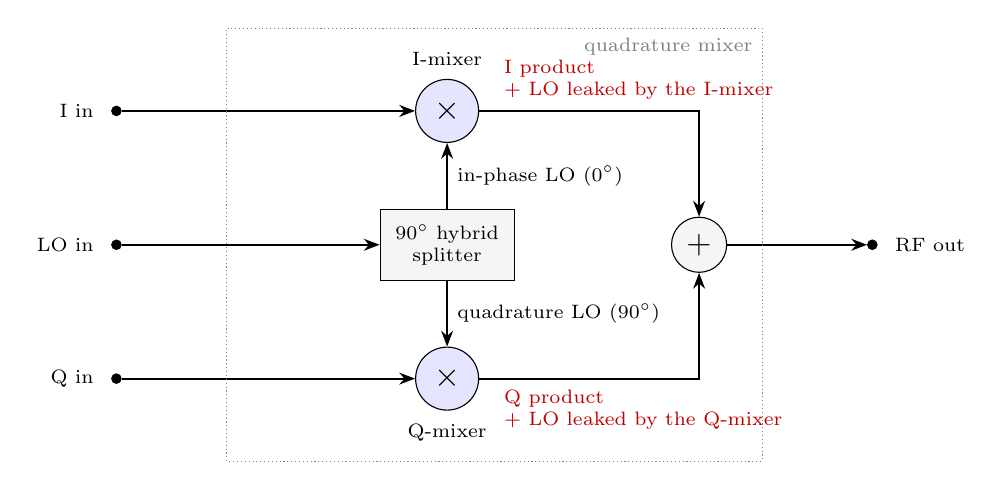
\begin{tikzpicture}[
  port/.style={draw, circle, fill=black, inner sep=1.2pt},
  mixer/.style={draw, circle, minimum size=8mm, inner sep=0pt, fill=blue!10, font=\large},
  sum/.style={draw, circle, minimum size=7mm, inner sep=0pt, fill=gray!8, font=\large},
  hyb/.style={draw, rectangle, minimum width=1.7cm, minimum height=0.9cm, align=center, font=\scriptsize, fill=gray!8},
  arr/.style={-{Stealth[length=2mm]}, thick},
  leak/.style={-{Stealth[length=1.8mm]}, thick, red!75!black, densely dashed},
  lbl/.style={font=\scriptsize, align=center}
]
\node[port] (iin) at (0, 1.7) {};
\node[port] (qin) at (0, -1.7) {};
\node[port] (loin) at (0, 0) {};
\node[lbl, left=1mm of iin] {I in};
\node[lbl, left=1mm of qin] {Q in};
\node[lbl, left=1mm of loin] {LO in};
\node[mixer] (mi) at (4.2, 1.7) {$\times$};
\node[mixer] (mq) at (4.2, -1.7) {$\times$};
\node[hyb] (hy) at (4.2, 0) {90$^\circ$ hybrid\\splitter};
\node[sum] (sm) at (7.4, 0) {$+$};
\node[port] (rfout) at (9.6, 0) {};
\node[lbl, right=1mm of rfout] {RF out};
\node[lbl, above=0.5mm of mi] {I-mixer};
\node[lbl, below=0.5mm of mq] {Q-mixer};
\draw[arr] (iin) -- (mi);
\draw[arr] (qin) -- (mq);
\draw[arr] (loin) -- (hy);
\draw[arr] (hy) -- node[lbl, right] {in-phase LO (0$^\circ$)} (mi);
\draw[arr] (hy) -- node[lbl, right] {quadrature LO (90$^\circ$)} (mq);
\draw[arr] (mi) -| (sm);
\draw[arr] (mq) -| (sm);
\draw[arr] (sm) -- (rfout);
\node[lbl, text=red!75!black, anchor=south west, align=left] at (4.8, 1.72) {I product\\+ LO leaked by the I-mixer};
\node[lbl, text=red!75!black, anchor=north west, align=left] at (4.8, -1.72) {Q product\\+ LO leaked by the Q-mixer};
\draw[densely dotted, gray] (1.4, -2.75) rectangle (8.2, 2.75);
\node[lbl, gray, anchor=north east] at (8.2, 2.75) {quadrature mixer};
\end{tikzpicture}
\captionof{figure}{A quadrature mixer used as an up-converter. The 90-degree hybrid splits the LO into an in-phase
copy, mixed with the I input, and a quadrature copy, mixed with the Q input; the two products are summed at the RF
output. Each mixer's output also carries some LO that the mixer leaks (red), so the LO leakage at
the RF output is the sum of what the two mixers leak.}\label{fig:6-qmix}
\end{center}

\textbf{What causes LO leakage, and why it matters.} The LO that each of the two mixers leaks into its output adds
up to a tone at the LO frequency at the RF port: the LO leakage. It does real harm. It is a strong, constant tone that
takes up output headroom in the amplifiers after the mixer, whatever is being transmitted, and a strong enough one can
drive the final amplifier into compression on its own. It also mixes with the transmitted signal in those amplifiers
(Section~\ref{sec:compression-upper}), and some of the resulting products land on the unwanted sideband,
worsening the sideband suppression of Section~\ref{sec:sideband-suppression}. And it puts real RF power at a frequency
the unit was never asked to transmit.

\textbf{A secondary source of LO leakage.} The LO is a strong signal inside the unit, and not all of the LO that
reaches the ``TX-side FR3 RF Out'' connector comes out of the mixer through the AM3153 filter. A small part reaches the
output by other paths that do not go through the filter. We see it directly in the measurements: in filter settings
that attenuate the LO frequency by 40\,dB or more, the LO leakage at the connector is no lower than in settings that
pass it. Because this part does not depend on the filter setting, it sets a floor under the LO leakage that no filter
setting can remove.

\textbf{How the bias cancels LO leakage.} Any DC voltage on the mixer's I and Q inputs also comes out at the LO
frequency. So a deliberate DC bias on those two lines --- two voltages this unit calls I\_V and Q\_V --- can be set to
produce a tone of the same size and opposite phase, cancelling the LO leakage. Plotted against I\_V and Q\_V, the
leakage power forms a smooth bowl with one minimum, and a search finds it: starting from I\_V~=~Q\_V~=~0\,V, it steps
on the I and Q axes, moves to whichever neighbouring point reads lowest, and halves the step whenever no neighbour is
lower. Once close to the bottom, a few nearby readings are used to fit the bowl's shape, and the minimum of that fit is
the nulled bias. Because the search minimizes the leakage measured at the ``TX-side FR3 RF Out'' connector, the bias it finds suppresses the total LO leakage at that output port, from both sources (the mixer and the secondary source), in the configuration the search was run in.

\textbf{Two sources, a very large search space.} For any one configuration --- a 5-dimensional search space of (FR1, FR3, sideband, filter setting, and temperature)
--- a search run in exactly that configuration finds the bias that cancels the \emph{total} LO leakage, from both
sources at once. But there are far too many configurations to calibrate each unit at the factory. The calibration
therefore makes one search per LO frequency (\calLoCount{} LO frequencies), in a single \emph{reference} filter setting,
at two different temperatures. The reference setting is, of the settings that can be in use at that LO frequency, the
one that passes the LO frequency with the least loss. There the mixer's leakage is
much stronger than the secondary leakage, so the null found there cancels the mixer's leakage. That one bias pair is
then used with every filter setting at that LO frequency: it keeps cancelling the mixer's leakage, but the secondary
leakage is not cancelled and comes through as it is. In most filter settings, the floor it sets is what is left. The
same bias pair serves both sidebands: we tested both, and the LO leakage did not change in any meaningful way between
them (the only changes were in readings already far below the \calThreshold\,dBm threshold).

\textbf{Factory calibration and temperature.} The bias that cancels the mixer's leakage drifts with temperature, and it
differs from unit to unit because it depends on each unit's own small circuit mismatches. Every unit is therefore
calibrated individually, on a 100\,MHz grid of LO frequencies from 7.0 to 22.5\,GHz (\calLoCount{} LO frequencies), at
two temperatures. FR1 and FR3 are chosen as multiples of 100\,MHz, so the LO always lands on a calibrated grid point.
Each LO frequency is calibrated at the LO drive it uses (\lmxDriveRule). The temperature is the LMX2820 synthesizer's
die temperature, from its built-in sensor: the ``cold'' calibration is made with the die at
\calColdMinC--\calColdMaxC\textdegree C and the ``hot'' one at \calHotMinC--\calHotMaxC\textdegree C. The unit's flash
stores one (I\_V, Q\_V) pair per LO frequency for each temperature (Figure~\ref{fig:6-3}), each with the die
temperature it was measured at. At runtime the unit applies it by itself: on every tune, and again every 2\,seconds,
its firmware reads the die temperature and interpolates between the cold and hot values (or extrapolates beyond them),
and sets the bias. Setting I\_V or Q\_V by hand switches this off; \texttt{IQBIAS AUTO} switches it back on
(Appendix~\ref{sec:commands}). The two temperatures matter because the null is very narrow. Between the cold and the hot calibration the stored bias moves by a median of \tdiffMedianMv\,mV (90\% of LO frequencies: \tdiffNinetyMv\,mV or less; up to \tdiffMaxMv\,mV), Figure~\ref{fig:6-4}, while in the reference setting a bias just 1\,mV off the null already raises the LO leakage by about \nullRiseOneMv\,dB, and 3\,mV off by about \nullRiseThreeMv\,dB. Using the cold bias on a hot unit, or the other way round, would therefore throw away most of the suppression; interpolating between the two tables by temperature keeps it. One
temperature's calibration takes about \calMinutesPerTemp{} minutes.\footnote{Disclaimer: these factory values are a
snapshot of the unit's behavior at calibration time; because they depend on small analog mismatches, they can change
over time, so a calibration should not be assumed valid indefinitely.}

\textbf{Pass criterion.} At each temperature, the calibration re-measures the LO leakage in every filter setting at
every LO frequency: \calReadCount{} readings, one per (LO frequency, filter setting) pair. It passes when at least
\calPassPct\% of them are at or below \calThreshold\,dBm at the ``TX-side FR3 RF Out'' connector.

\textbf{What you get.} Figures~\ref{fig:6-1} and~\ref{fig:6-1h} show the LO leakage after the cold and the hot
calibration. Read them one LO frequency at a time: the line is the median across the filter settings usable at that LO
frequency, and the shaded band spans the best setting to the worst. Where the top of the band stays below the dashed
\calThreshold\,dBm line, every setting passes. The reference setting is left out: the leakage there is far lower than in
any other setting (median \calRefMedian\,dBm). Figure~\ref{fig:6-2} shows all the readings as histograms. In the cold
calibration, \calColdPct\% of the readings are at or below \calThreshold\,dBm (median \calColdMedian\,dBm, worst
\calColdWorst\,dBm); in the hot calibration, \calHotPct\% (median \calHotMedian\,dBm, worst \calHotWorst\,dBm).

\textbf{Your unit will differ --- and you can do better yourself.} On your own unit, Figure~\ref{fig:6-1} may look quite
different: the leakage drifts, and one stored bias pair per LO frequency has to serve every filter setting. If LO
leakage matters for your experiment, set the unit up exactly as your experiment uses it (the same FR1, FR3, sideband, and filter setting), run the search described above on the LO leakage at the ``TX-side FR3 RF Out'' connector, and set
the result with the \texttt{SET I\_V} and \texttt{SET Q\_V} commands (Section~\ref{sec:commands}), which also
switch the automatic bias off, so it stays put. In that one
configuration, the search cancels the total LO leakage, including the secondary leakage that the factory calibration
leaves in place.

\clearpage
% the three LO-suppression figures together on one page, each in its own full-width row (user layout, 2026-10-05)
\begin{center}\begin{minipage}{\linewidth}\centering% graphic and caption kept together
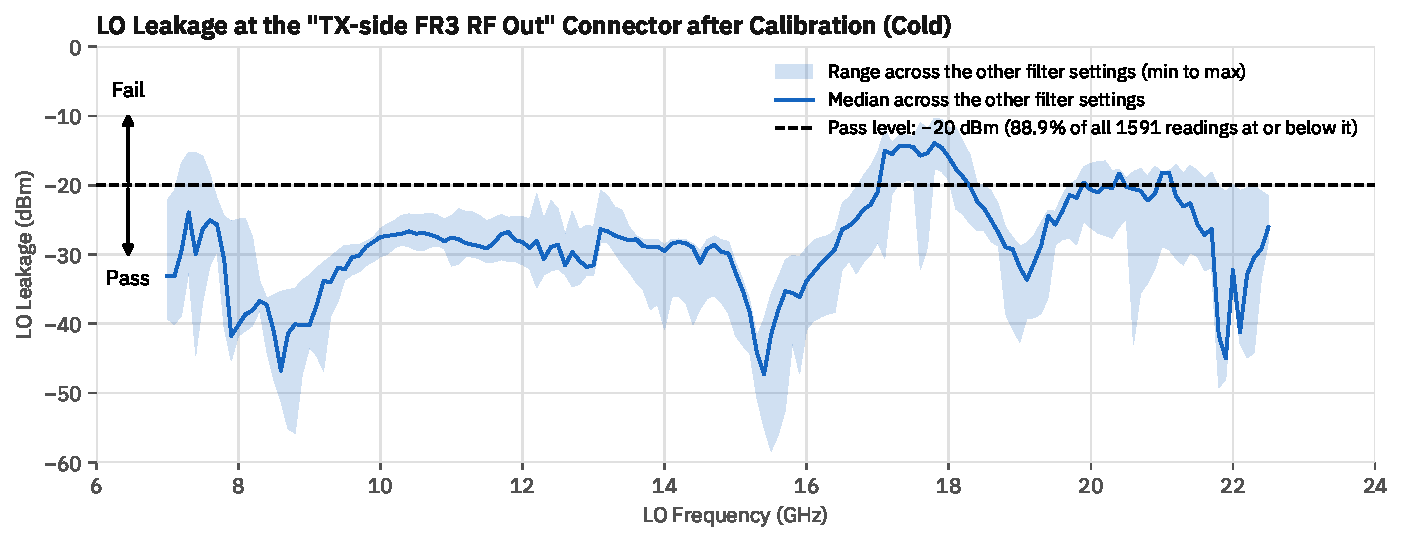
\includegraphics[width=\linewidth]{images/sec6_cal_fig1.pdf}
\captionof{figure}{LO leakage at the ``TX-side FR3 RF Out'' connector after the cold calibration, at each of the
\calLoCount{} calibrated LO frequencies (100\,MHz steps). At each LO frequency, the stored bias pair was applied and
the LO leakage was measured in every filter setting that can be in use at that LO frequency, other than the
reference setting the null was found in. The line is the median of those readings, and the shaded band spans the
lowest to the highest of them. The dashed line is the \calThreshold\,dBm pass level.}\label{fig:6-1}
\end{minipage}\end{center}
\vspace{-0.8em}
\begin{center}\begin{minipage}{\linewidth}\centering% graphic and caption kept together
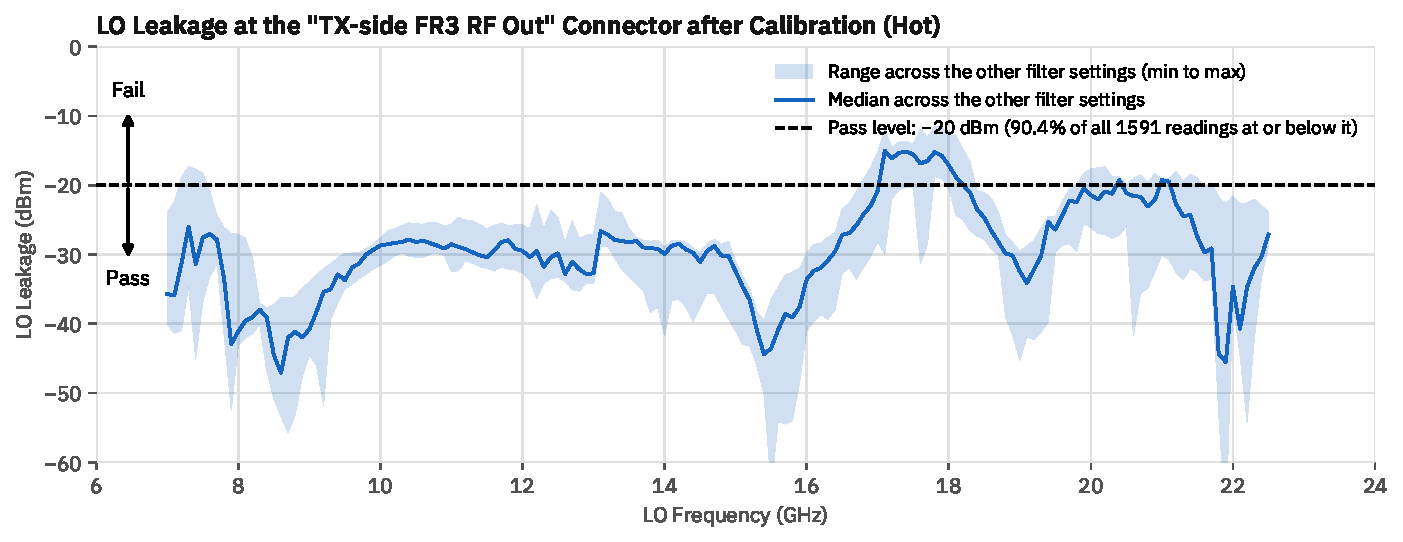
\includegraphics[width=\linewidth]{images/sec6_cal_fig1_hot.pdf}
\captionof{figure}{The same as Figure~\ref{fig:6-1}, after the hot calibration (LMX die at
\calHotMinC--\calHotMaxC\textdegree C).}\label{fig:6-1h}
\end{minipage}\end{center}
\vspace{-0.8em}
\begin{center}\begin{minipage}{\linewidth}\centering% graphic and caption kept together
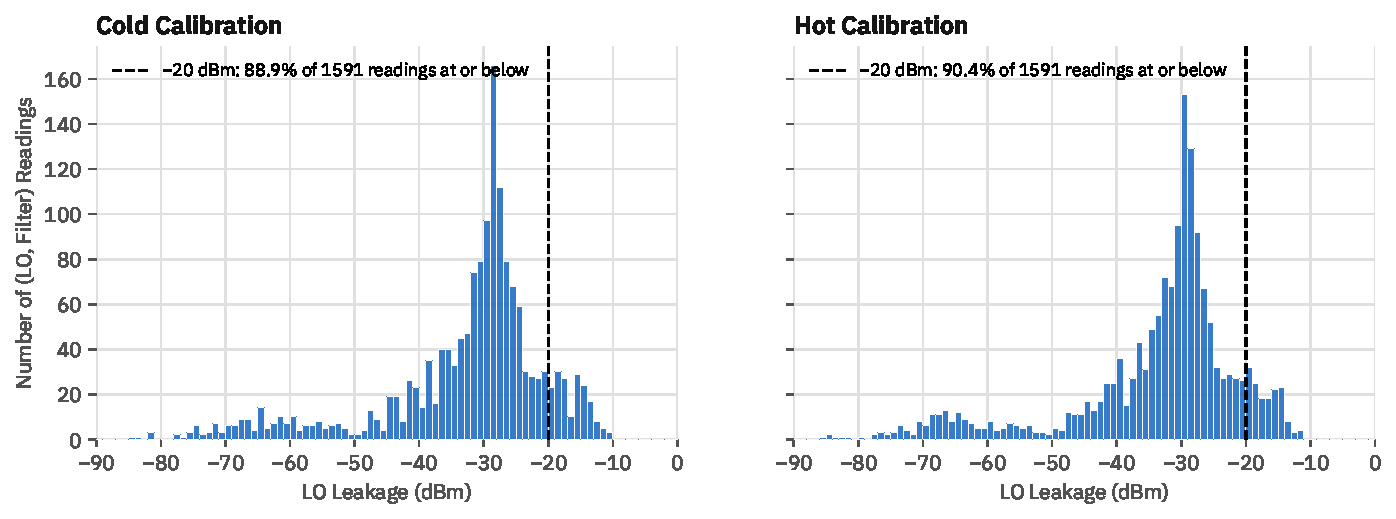
\includegraphics[width=\linewidth]{images/sec6_cal_fig2.pdf}
\captionof{figure}{All the readings of the cold and the hot calibration as histograms: the number of (LO frequency, filter setting)
readings, the reference setting included, at each level of LO leakage, in 1\,dB bins. The dashed line is the
\calThreshold\,dBm pass level; a calibration passes when at least \calPassPct\% of the readings are at or below
it.}\label{fig:6-2}
\end{minipage}\end{center}
\vspace{-0.8em}
\begin{center}\begin{minipage}{\linewidth}\centering% graphic and caption kept together
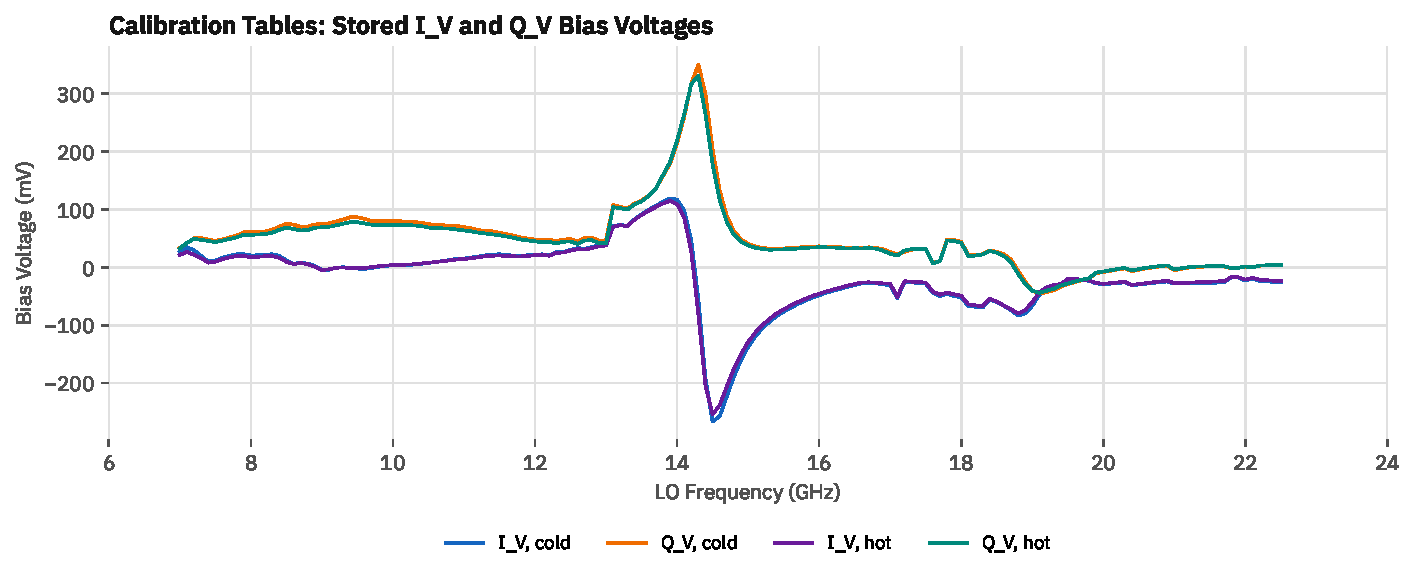
\includegraphics[width=\linewidth]{images/sec6_cal_fig3.pdf}
\captionof{figure}{The unit's two calibration tables: at each LO frequency (100\,MHz steps), the I\_V and Q\_V bias
voltages stored in flash. Cold: recorded with the LMX die at \calColdMinC--\calColdMaxC\textdegree C. Hot: recorded
with the LMX die at \calHotMinC--\calHotMaxC\textdegree C. At runtime the bias is interpolated between
these.}\label{fig:6-3}
\end{minipage}\end{center}
\vspace{-0.8em}
\begin{center}\begin{minipage}{\linewidth}\centering% graphic and caption kept together
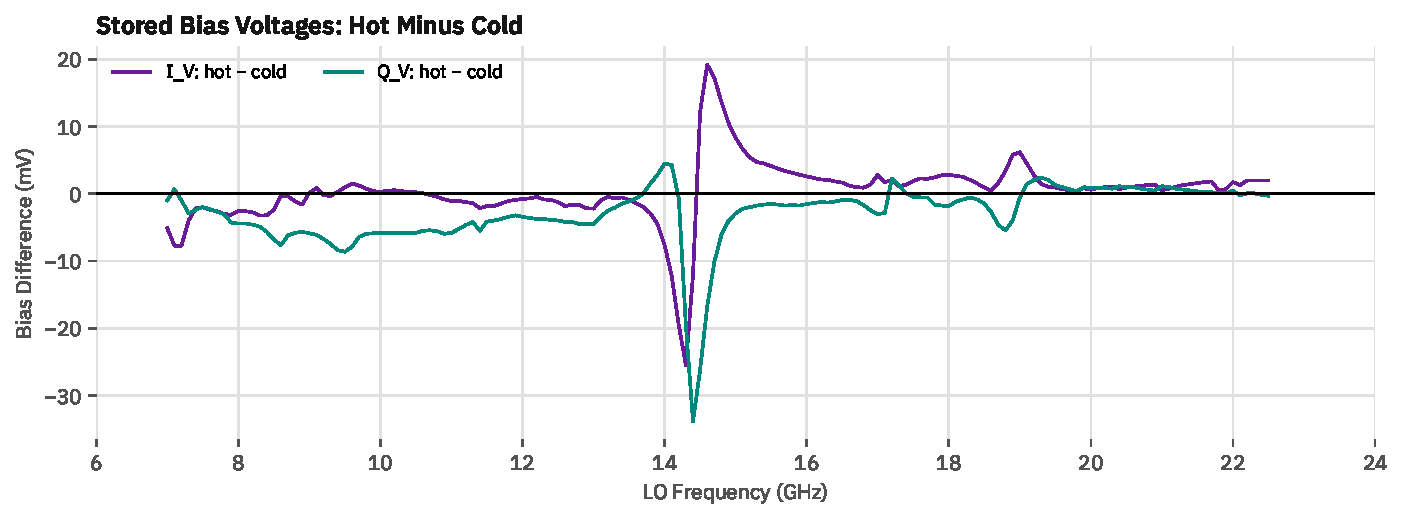
\includegraphics[width=\linewidth]{images/sec6_cal_fig4.pdf}
\captionof{figure}{The difference between the two calibration tables of Figure~\ref{fig:6-3}: hot minus cold, for I\_V and Q\_V, at each LO frequency. A few mV is enough to change the LO leakage by tens of dB, which is why the bias is interpolated by temperature at runtime.}\label{fig:6-4}
\end{minipage}\end{center}

\clearpage
\section{Spurious Outputs}
\label{sec:spurious-outputs}
\raggedbottom% short text pages end short instead of stretching the gaps (the figure follows on its own)
% numbers: sections/sec_spur_numbers.tex, loaded in the Key Specifications section (it is quoted there first)

Besides the signal you ask it to transmit, every real transmitter also puts out small, unwanted tones at other
frequencies. These are called spurious outputs, or ``spurs''. A spur carries no information; it is simply RF energy
at a frequency you did not ask for. Spurs matter for two reasons: they can interfere with other radios (including
other Pi-Radio units) that are listening at the spur's frequency, and they count against the spectrum-emission
limits that apply whenever a transmitter is connected to an antenna. This section lists the spurs we have
characterized on this unit.

\subsection{TX-side 2×LO Spur}
\label{sec:spur-tx-2lo}

\textbf{What it is.} The LO is a strong signal inside the unit, and every real oscillator and amplifier produces
harmonics of its signal. Some of the second harmonic of
the LO, at exactly twice the LO frequency (``2×LO''), appears at the ``TX-side FR3 RF Out'' connector as a spur.
Its frequency depends only on the LO, so to find it, first work out the LO from your FR1 and FR3 settings: for the
upper sideband, LO~=~FR3~$-$~FR1; for the lower sideband, LO~=~FR3~+~FR1. For example, FR1~=~1\,GHz and
FR3~=~9\,GHz in the upper sideband gives LO~=~8\,GHz, so the 2×LO spur is at 16\,GHz. The spur is always well
away from the wanted signal, but it can land inside the 6--24\,GHz FR3 band, where another unit or receiver may be
working.

\textbf{How we measured it.} At each of \twoLoLoCount{} LO frequencies from \twoLoLoMin{} to \twoLoLoMax\,GHz, in 100\,MHz steps, with nothing connected to the ``TX-side FR1 IF In'' port, the LO leakage was first nulled with the reference filter, exactly as in the calibration of Section~\ref{sec:lo-suppression}. The power at 2×LO was then read at the ``TX-side FR3 RF Out'' connector (cable loss removed) in \emph{every} filter setting that can be in use at that LO frequency --- every setting the optimal-filter rule can select for any FR1 from 0.7 to 4.0\,GHz, in either sideband --- \twoLoReadCount{} readings in all. The unit was measured hot, as the worst case (no fan, LMX2820 die at \twoLoMinC--\twoLoMaxC\textdegree C), with \lmxDriveRule.

\textbf{What you get.} Figure~\ref{fig:spur-1} shows the result: at each LO frequency, the median over all the filter settings and the range from the lowest to the highest. The median of all \twoLoReadCount{} readings is \twoLoMedian\,dBm. The filter setting makes a large difference, often 20\,dB or more at the same LO frequency. The highest reading is \twoLoMax\,dBm (LO~=~\twoLoMaxLo\,GHz, filter \twoLoMaxFilter); only \twoLoAboveTwenty{} of the \twoLoReadCount{} readings are above $-$20\,dBm, all of them at LO frequencies from \twoLoAboveLoMin{} to \twoLoAboveLoMax\,GHz. The level also changes quickly from one LO frequency to the next, so read the figure as an envelope rather than as an exact value at any one frequency.

\textbf{What it does not depend on.} The spur level does not depend on the signal you transmit: with a 1\,GHz
input tone switched on after the LO was nulled, the 2×LO spur changed by less than 1\,dB at \spurToneWithinOne{}
of \spurToneCount{} LO frequencies (median change \spurToneMedianDiff\,dB). It also does not depend on how well the
LO leakage is nulled, as long as the LO leakage itself stays below about $-$10\,dBm. Above that, the spur grows
quickly: with the LO leakage deliberately raised to +10\,dBm, the 2×LO spur rose to between \spurAmpLow{} and
\spurAmpHigh\,dBm, and with the LO leakage left uncorrected (I\_V~=~Q\_V~=~0\,V, LO leakage up to
+\spurZeroBiasLoMax\,dBm) it reached \spurZeroBiasWorst\,dBm. Keeping the LO-leakage calibration of
Section~\ref{sec:lo-suppression} applied therefore also keeps the 2×LO spur at the levels of
Figure~\ref{fig:spur-1}.

\textbf{Variation between units.} These results are from one unit. We expect differences of a few dB from one unit to the next, and expect the 2×LO spur to stay below $-$20\,dBm on any unit for a vast majority of configurations.

\textbf{Measurement limit.} For LO frequencies above \spurLoLimit\,GHz, the 2×LO spur lies above
\spurTwoLoLimit\,GHz, which is the rated limit of the unit's SMA connectors and of the test equipment we used; it
was not measured there.

\textbf{Practical advice.} For cabled measurements, where your receiver or analyzer is tuned to the FR3 frequency,
the 2×LO spur usually needs no action. When you transmit over the air with a wideband antenna, or share the band
with other receivers that may be tuned near 2×LO, add an external low-pass or band-pass filter after the
``TX-side FR3 RF Out'' connector that passes your FR3 frequency and blocks 2×LO.

\begin{center}
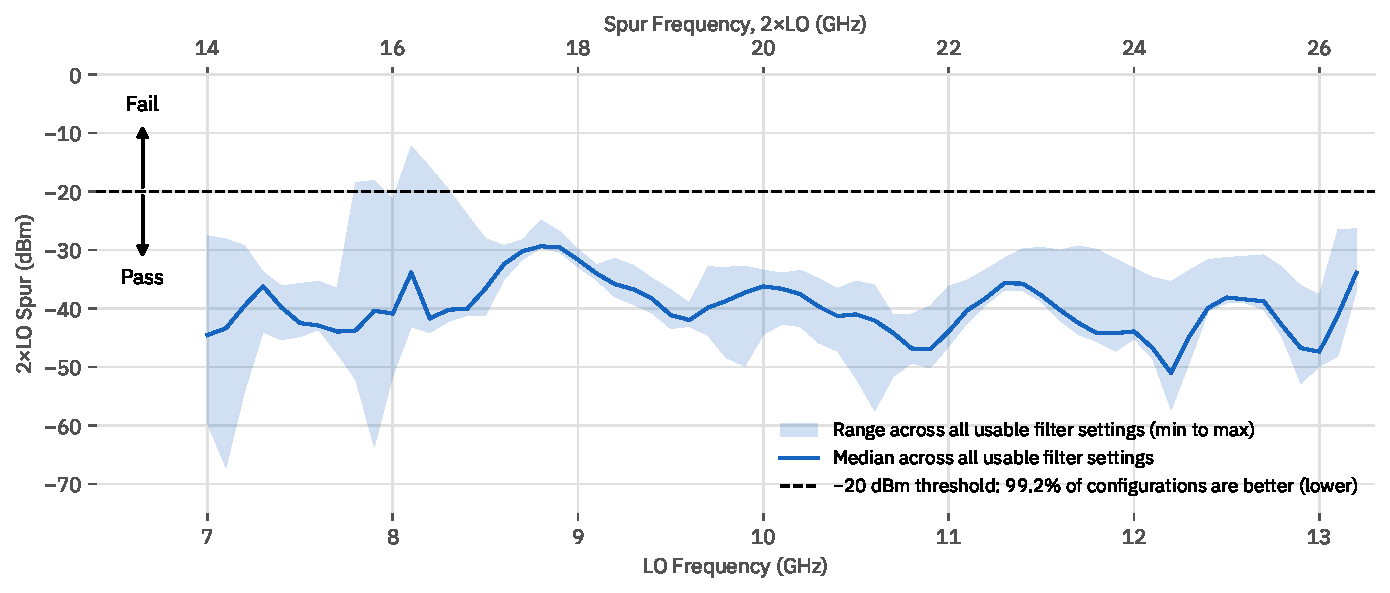
\includegraphics[width=\linewidth]{images/sec_spur_2lo_all_filters.pdf}
\captionof{figure}{TX-side 2×LO spur at the ``TX-side FR3 RF Out'' connector at \twoLoLoCount{} LO frequencies (\twoLoLoMin--\twoLoLoMax\,GHz in 100\,MHz steps; top axis: the spur frequency, 2×LO). At each LO frequency the LO leakage was nulled with the reference filter, and the 2×LO was read in every filter setting usable at that LO frequency, with no input signal. The line is the median across those settings, and the shaded band spans the lowest to the highest. The dashed line marks $-$20\,dBm.}\label{fig:spur-1}
\end{center}
\subsection{RX-side LO and 2×LO Leakage}
\label{sec:spur-rx-lo}

\textbf{Why it matters.} The RX side is meant only to receive, but the LO is running inside the unit the whole time,
and a little of it, along with its second harmonic (2×LO), leaks backwards out of the ``RX-side FR3 RF In''
connector. With a cable to a signal generator or another unit this does no harm. With an antenna connected, however,
whatever leaks out of that connector is radiated: the unit transmits a weak tone at the LO frequency, and another at
2×LO, even while it is only receiving. Those tones can interfere with other receivers nearby (including other
Pi-Radio units in the same experiment), and they count against the emission limits that apply to anything connected
to an antenna.

\textbf{How we measured it.} At each LO frequency, the unit was set up as it would be in normal use: \lmxDriveRule{} (set from the LO frequency); the TX side with its stored LO-leakage calibration applied and its optimal filter engaged (with the ``TX-side FR3 RF Out'' connector terminated in 50\,$\Omega$); and the RX filter in its ``optimal'' state for FR3~=~LO~+~1\,GHz. Nothing else was connected. A spectrum analyzer on the ``RX-side FR3 RF In'' connector (cable loss removed) read the power at the LO frequency and at 2×LO. The LO leakage was measured at \rxLeakLoCount{} LO frequencies from \rxLeakLoMin{} to \rxLeakLoTop\,GHz in 100\,MHz steps; 2×LO was measured at the \rxLeakTwoLoCount{} LO frequencies up to \rxLeakLoFineMax\,GHz, where 2×LO stays within \spurTwoLoLimit\,GHz. The unit was measured hot: no fan, LMX2820 die at \rxLeakLmxMinC--\rxLeakLmxMaxC\textdegree C.

\textbf{What you get.} Figure~\ref{fig:spur-2} shows the LO leakage, and Figure~\ref{fig:spur-3} the 2×LO leakage.
The LO leakage out of the ``RX-side FR3 RF In''
connector has a median of \rxLeakLoMedian\,dBm and reaches at most \rxLeakLoMax\,dBm (at LO~=~\rxLeakLoMaxAt\,GHz).
The 2×LO leakage has a median of \rxLeakTwoLoMedian\,dBm and reaches at most \rxLeakTwoLoMax\,dBm (at
LO~=~\rxLeakTwoLoMaxAt\,GHz). The LO leakage is lowest at the bottom of the LO range (\rxLeakLoBest\,dBm at
LO~=~\rxLeakLoBestAt\,GHz) and highest in the middle of it, around LO~=~\rxLeakLoMaxAt\,GHz. As for the TX-side spur,
these results are from one unit, and we expect differences of a few dB from one unit to the next.

\textbf{It does not depend on the TX-side calibration.} At \rxLeakOffsetCount{} of the LO frequencies
(\rxLeakOffsetLos\,GHz) we repeated the reading with the TX LO-leakage bias deliberately moved \rxLeakOffsetMv\,mV
away from its null, which raises the TX-side LO leakage by tens of dB. The leakage out of the ``RX-side FR3 RF In''
connector changed by at most \rxLeakOffsetMaxChange\,dB. So the RX-side leakage does not depend on how well the TX side
is calibrated, or on the TX side's calibration drifting with time and temperature.

\textbf{Measurement limit.} For LO frequencies above \spurLoLimit\,GHz, 2×LO lies above \spurTwoLoLimit\,GHz, the
rated limit of the unit's SMA connectors and of our test equipment, and was not measured there.

\textbf{Practical advice.} If you receive through an antenna and the leakage matters for your experiment, add a
band-pass filter between the antenna and the ``RX-side FR3 RF In'' connector that passes your FR3 frequency and
rejects the LO. Because the LO is exactly FR1 away from FR3, choosing a larger FR1 moves the LO further from your
signal and makes such a filter easier to build.

\noindent\begin{minipage}{\linewidth}
\centering
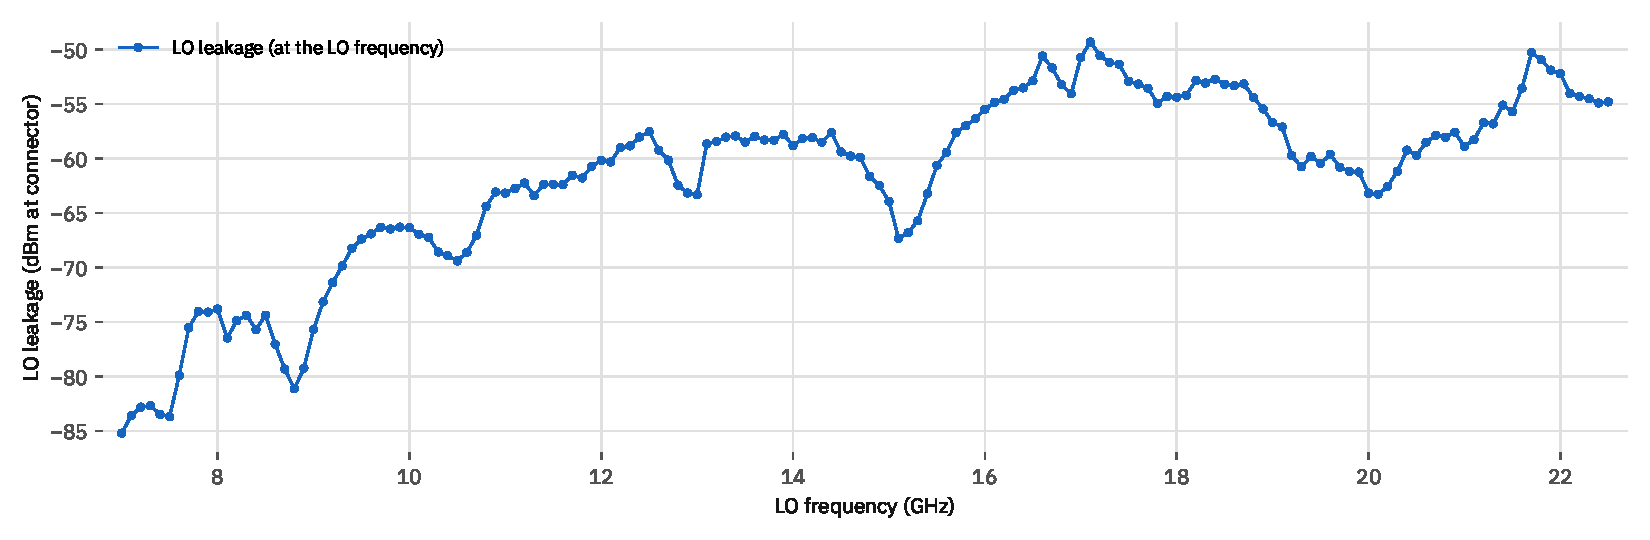
\includegraphics[width=\linewidth]{images/sec_spur_fig2.pdf}
\captionof{figure}{LO leakage at the ``RX-side FR3 RF In'' connector against LO frequency. LMX2820 drive rule; TX side in normal use (stored LO-leakage calibration, optimal filter), ``TX-side FR3 RF Out'' terminated in 50\,$\Omega$; RX filter optimal for FR3~=~LO~+~1\,GHz; nothing else connected.}\label{fig:spur-2}
\end{minipage}

\bigskip
\noindent\begin{minipage}{\linewidth}
\centering
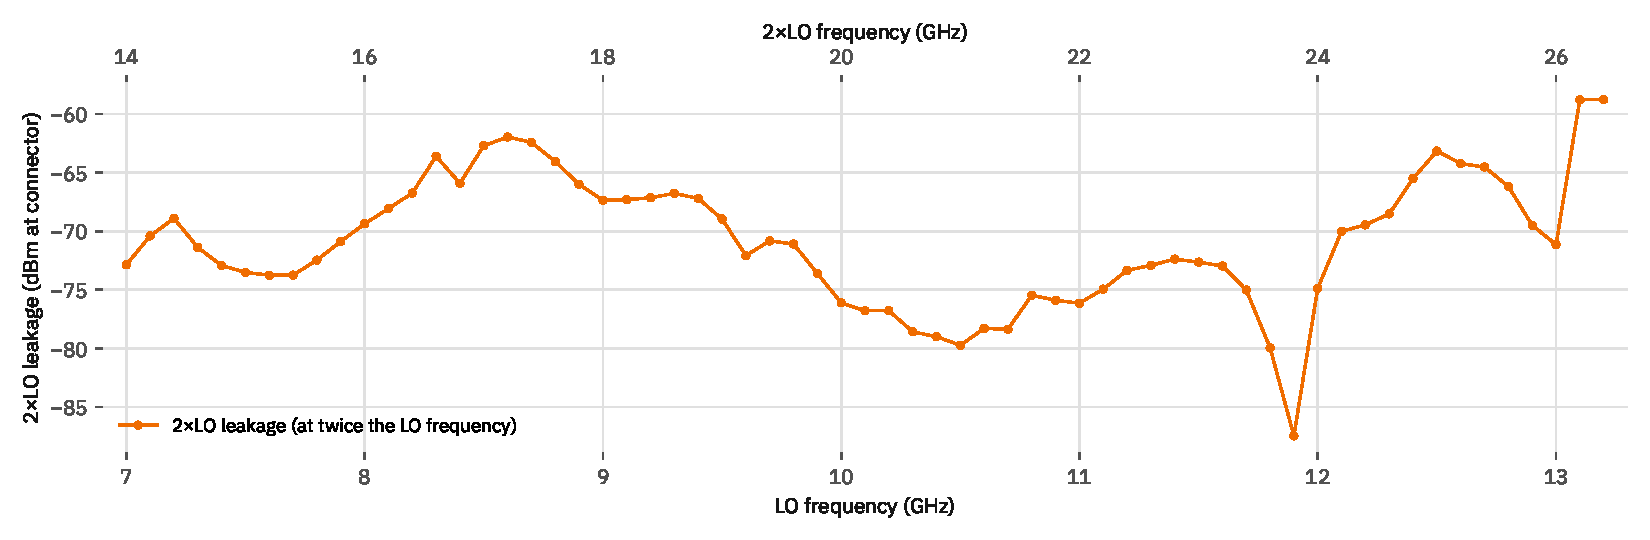
\includegraphics[width=\linewidth]{images/sec_spur_fig3.pdf}
\captionof{figure}{2×LO leakage at the ``RX-side FR3 RF In'' connector against LO frequency (top axis: the 2×LO frequency), in the same set-up as Figure~\ref{fig:spur-2}. Measured for LO up to \rxLeakLoFineMax\,GHz: above \spurLoLimit\,GHz, 2×LO would exceed \spurTwoLoLimit\,GHz, the limit of the connectors and test equipment.}\label{fig:spur-3}
\end{minipage}

\flushbottom

\clearpage
\section{RX-side Conversion Gain --- Low-Side LO (No Spectral Flip)}
\label{sec:rx-gain-lowside}

\textbf{What is conversion gain?} The RX side is the TX side in reverse: it takes a signal in at a high FR3
frequency and brings it down to FR1, amplifying it along the way. Conversion gain measures that amplification
across the change of frequency. Feed a signal into the ``RX-side FR3 RF In'' connector at, say, −50\,dBm, and
measure the signal that comes out of the ``RX-side FR1 IF Out'' connector at its new frequency, say −5\,dBm. The conversion
gain is simply the difference: −5 − (−50) = 45\,dB. Because both powers are in dBm, subtracting them gives the
conversion gain in dB directly.

\textbf{What's plotted.} Each of the first seven figures holds FR1 (the IF output frequency) fixed at one
center value (1.0 up to the unit's 4.0\,GHz maximum, in 0.5\,GHz steps) and plots conversion gain against the
swept FR3 input frequency for that output, using the same methodology as the TX conversion-gain sections: every
point is the average conversion gain across a real 500\,MHz swept window centered on that point, not a single
CW tone.\footnote{The FieldFox's built-in tracking generator drives FR3 into the ``RX-side FR3 RF In'' port at a
calibrated
−50\,dBm while its own receiver sweeps the corresponding FR1 window at the ``RX-side FR1 IF Out'' port
in lock-step.} Grey is the raw LNA-and-mixer chain with the AM3153 filter bypassed; blue is the filter engaged,
re-selected at every point using the same ``optimal'' algorithm described in
Section~\ref{sec:sideband-suppression}, reused here because the AM3153 is RX's actual image-rejection mechanism
--- there is no I/Q image rejection on this side of the board, since the mixer's Q output is simply discarded.

\textbf{Measurement conditions.} \lmxDriveRule{} (set from the LO frequency). Because the LO is shared, the TX side was set up at every point exactly as in normal use (its stored LO-leakage calibration applied and its optimal filter engaged), with both TX-side ports terminated in 50\,\textohm. The unit was measured hot, as on the TX side: no fan, LMX2820 die at \condRxGainMinC--\condRxGainMaxC\textdegree C.

\textbf{How the filter is chosen.} The same two-step rule used throughout this datasheet: first find whichever
of the 48 candidate configurations (3 bands × 16 sub-states) passes the most desired energy on its own;
then, restricted to candidates within 3\,dB of that best desired power, choose whichever rejects the image the
most. Consecutive points that land on the same filter form a \emph{region}; the dashed vertical lines on each
panel mark every boundary between regions, and the blue hex code running up from the x-axis inside each region
is the actual \texttt{filter\_bits} value used for every point in it.

\textbf{Low-side LO: LO = FR3 − FR1.} This is the LO tuning regime shown in this section. Because of it, the
IF output spectrum is \emph{not} flipped relative to the RF input --- as FR3 increases, the IF output's own
internal content increases too.\footnote{Since TX and RX share one physical LO, this also means the two
chains' LO-side states are always consistent with each other: whenever RX is running low-side LO, TX (if active at the
same time) is necessarily running upper-sideband up-conversion, and vice versa.} In Figure~\ref{fig:7-7} (FR1 = 4.0\,GHz), as on the TX side, the window extends 250\,MHz past the unit's IF design spec. Figures~\ref{fig:7-8} and~\ref{fig:7-9} repeat the bypassed and optimal data across the full (FR1, FR3) grid.

\figpair{images/sec7_fig1.pdf}{FR1 (output) = 1.0\,GHz.}{fig:7-1}%
        {images/sec7_fig2.pdf}{FR1 (output) = 1.5\,GHz.}{fig:7-2}

\figpair{images/sec7_fig3.pdf}{FR1 (output) = 2.0\,GHz.}{fig:7-3}%
        {images/sec7_fig4.pdf}{FR1 (output) = 2.5\,GHz.}{fig:7-4}
\figpair{images/sec7_fig5.pdf}{FR1 (output) = 3.0\,GHz.}{fig:7-5}%
        {images/sec7_fig6.pdf}{FR1 (output) = 3.5\,GHz.}{fig:7-6}
\figonesmall{images/sec7_fig7.pdf}{FR1 (output) = 4.0\,GHz. 250\,MHz of this window falls outside the unit's IF design spec (shown in red).}{fig:7-7}

\newpage
\figrow{images/sec7_fig8.pdf}{Conversion gain, low-side LO: full measured (FR1, FR3) grid, filter bypassed.
Zoom in to read each cell's exact values, printed as (FR1, FR3, conversion gain), with FR1 and FR3 in GHz and
the conversion gain in dB.}{fig:7-8}
\figrow{images/sec7_fig9.pdf}{Conversion gain, low-side LO: full measured (FR1, FR3) grid, optimal filter.
Zoom in to read each cell's exact values, printed as (FR1, FR3, conversion gain), with FR1 and FR3 in GHz and
the conversion gain in dB.}{fig:7-9}

\clearpage
\section{RX-side Conversion Gain --- High-Side LO (Spectral Flip)}
\label{sec:rx-gain-highside}

\textbf{What is conversion gain?} Exactly as in Section~\ref{sec:rx-gain-lowside}: the power of the signal
coming out of the ``RX-side FR1 IF Out'' connector, minus the power of the signal fed into the ``RX-side FR3 RF In'' connector, both in dBm,
gives the conversion gain in dB. Only the LO's position changes here, now above FR3 instead of below it.

\textbf{What's plotted.} Identical methodology to Section~\ref{sec:rx-gain-lowside}, with the unit tuned to
high-side LO instead: each of the first seven figures holds FR1 (the IF output frequency) fixed at one center
value (1.0 up to the unit's 4.0\,GHz maximum, in 0.5\,GHz steps) and plots conversion gain against the swept
FR3 input frequency for that output, using the same methodology as the TX conversion-gain sections: every point
is the average conversion gain across a real 500\,MHz swept window centered on that point, not a single CW
tone.\footnote{Every point is the average conversion gain across a real 500\,MHz swept window, at a calibrated
−50\,dBm input level, same as Section~\ref{sec:rx-gain-lowside}.} Grey is the raw LNA-and-mixer chain with
the AM3153 filter bypassed; blue is the filter engaged, re-selected at every point using the same ``optimal''
algorithm described in Section~\ref{sec:sideband-suppression}, reused here because the AM3153 is RX's actual
image-rejection mechanism --- there is no I/Q image rejection on this side of the board, since the mixer's Q
output is simply discarded. The gap between the two traces, at any point, is exactly how much the filter costs
in insertion loss there, same as on the TX-side gain sections.

\textbf{Measurement conditions.} The same as in Section~\ref{sec:rx-gain-lowside} (the same run): LMX2820 die at \condRxGainMinC--\condRxGainMaxC\textdegree C.

\textbf{How the filter is chosen.} The same two-step rule used throughout this datasheet: first find whichever
of the 48 candidate configurations (3 bands × 16 sub-states) passes the most desired energy on its own;
then, restricted to candidates within 3\,dB of that best desired power, choose whichever rejects the image the
most. Consecutive points that land on the same filter form a \emph{region}; the dashed vertical lines on each
panel mark every boundary between regions, and the blue hex code running up from the x-axis inside each region
is the actual \texttt{filter\_bits} value used for every point in it --- so, exactly as on the TX side, the
exact filter behind any measurement on these panels is always readable directly off the figure, with no need to
consult a separate table.

\textbf{High-side LO: LO = FR3 + FR1.} This is the LO tuning regime shown in this section. Because of it,
the IF output spectrum \emph{is} flipped (mirrored) relative to the RF input --- as FR3 increases, the IF
output's own internal content decreases.\footnote{Since TX and RX share one physical LO, whenever RX is
running high-side LO, TX (if active at the same time) is necessarily running lower-sideband up-conversion, and
vice versa.} Every point's window is exactly 500\,MHz wide, the same fixed window used throughout the TX-side
gain sections: a fixed filter setting's measured response across that full window is exactly what a real
wideband signal at that setting would experience. Figure \ref{fig:8-7} (FR1 = 4.0\,GHz) is the one exception,
just as on the TX side: its window extends 250\,MHz past the unit's IF design spec, called out directly on
that panel and outlined in red on Figures \ref{fig:8-8} and \ref{fig:8-9}, which repeat the bypassed and
optimal data across the full measured (FR1, FR3) grid for a single-glance view instead of the seven separate
slices above.

\figpair{images/sec8_fig1.pdf}{FR1 (output) = 1.0\,GHz.}{fig:8-1}%
        {images/sec8_fig2.pdf}{FR1 (output) = 1.5\,GHz.}{fig:8-2}

\figpair{images/sec8_fig3.pdf}{FR1 (output) = 2.0\,GHz.}{fig:8-3}%
        {images/sec8_fig4.pdf}{FR1 (output) = 2.5\,GHz.}{fig:8-4}
\figpair{images/sec8_fig5.pdf}{FR1 (output) = 3.0\,GHz.}{fig:8-5}%
        {images/sec8_fig6.pdf}{FR1 (output) = 3.5\,GHz.}{fig:8-6}
\figonesmall{images/sec8_fig7.pdf}{FR1 (output) = 4.0\,GHz. 250\,MHz of this window falls outside the unit's IF design spec (shown in red).}{fig:8-7}

\newpage
\figrow{images/sec8_fig8.pdf}{Conversion gain, high-side LO: full measured (FR1, FR3) grid, filter bypassed.
Zoom in to read each cell's exact values, printed as (FR1, FR3, conversion gain), with FR1 and FR3 in GHz and
the conversion gain in dB.}{fig:8-8}
\figrow{images/sec8_fig9.pdf}{Conversion gain, high-side LO: full measured (FR1, FR3) grid, optimal filter.
Zoom in to read each cell's exact values, printed as (FR1, FR3, conversion gain), with FR1 and FR3 in GHz and
the conversion gain in dB.}{fig:8-9}

\clearpage
\section{RX-side Gain Flatness}
\label{sec:rx-flatness}
\raggedbottom% no stretched gaps between text and figures (as in the NF section)

\textbf{What is gain flatness?} Exactly as on the TX side (Section~\ref{sec:tx-flatness}): how much the conversion
gain varies \emph{within} a 500\,MHz window, rather than its average (Sections~\ref{sec:rx-gain-lowside} and
\ref{sec:rx-gain-highside}). A received wideband signal that passes through an uneven channel comes out of the unit
with a tilted or rippled spectrum.

\textbf{How it's measured.} The same way as on the TX side, with the roles of the ports swapped: at every (FR1, FR3)
point, the FieldFox's tracking generator sweeps the FR3 window into the ``RX-side FR3 RF In'' port, while its
receiver follows the 500\,MHz window centred on FR1 at the ``RX-side FR1 IF Out'' port, in 101 steps 5\,MHz apart.
The input level is −50\,dBm, the same as in the RX conversion-gain sections, low enough to keep the highest-gain
points clear of compression, which would flatten the measured ripple. The signal level arriving at the
unit was again measured directly, by connecting the FieldFox's source to its own receiver through the same input
cable, and the output cable's loss is removed from its own calibration. Each window is measured with the AM3153
filter bypassed and with the ``optimal'' filter, never changing the filter during a sweep, over the same grid as on
the TX side, for both low-side and high-side LO. The number reported is the RMS flatness defined in
Section~\ref{sec:tx-flatness}: 0\,dB is perfectly flat, and in this data the peak-to-peak spread in a window is
typically about \flatRxPpRatio{} times the RMS flatness (between \flatRxPpRatioLow{} and \flatRxPpRatioHigh{} times
at 80\% of the points).

\textbf{Measurement conditions.} \lmxDriveRule{} (set from the LO frequency). Because the LO is shared, the TX side was set up at every point exactly as in normal use (its stored LO-leakage calibration applied and its optimal filter engaged), with both TX-side ports terminated in 50\,\textohm. The unit was measured hot, as on the TX side: no fan, LMX2820 die at \condRxFlatMinC--\condRxFlatMaxC\textdegree C.

\textbf{Results.} Within the design spec (FR3~$\le$~24\,GHz, and FR1 centre~$\le$~3.5\,GHz):
\par\medskip\noindent\begin{minipage}{\linewidth}% caption and table stay on one page
\begin{center}
\captionof{table}{RX-side RMS gain flatness within the design spec, by LO side and filter setting.}\label{tab:rxflat-results}
\vspace{0.4em}
\begin{tabular}{lcccc}
\toprule
 & Median & 90\% of points at or below & Best & Worst \\
\midrule
Low-side LO, filter bypassed & \flatRxLowBypassMedian\,dB & \flatRxLowBypassPninety\,dB & \flatRxLowBypassMin\,dB & \flatRxLowBypassMax\,dB \\
Low-side LO, optimal filter & \flatRxLowOptimalMedian\,dB & \flatRxLowOptimalPninety\,dB & \flatRxLowOptimalMin\,dB & \flatRxLowOptimalMax\,dB \\
High-side LO, filter bypassed & \flatRxHighBypassMedian\,dB & \flatRxHighBypassPninety\,dB & \flatRxHighBypassMin\,dB & \flatRxHighBypassMax\,dB \\
High-side LO, optimal filter & \flatRxHighOptimalMedian\,dB & \flatRxHighOptimalPninety\,dB & \flatRxHighOptimalMin\,dB & \flatRxHighOptimalMax\,dB \\
\bottomrule
\end{tabular}
\end{center}
\end{minipage}\par

\textbf{Where it's flattest, and how to use that.} The median per FR1 centre (all FR3 up to 24\,GHz):
\par\medskip\noindent\begin{minipage}{\linewidth}% caption and table stay on one page
\begin{center}
\captionof{table}{RX-side median RMS gain flatness for each FR1 centre (all FR3 up to 24\,GHz).}\label{tab:rxflat-by-fr1}
\vspace{0.4em}
\footnotesize
% Generated by FR3_Characterization/plot_datasheet_flatness.py -- do not edit by hand.
\begin{tabular}{lcccc}
\toprule
FR1 centre & Low-side LO, bypassed & Low-side LO, optimal & High-side LO, bypassed & High-side LO, optimal \\
\midrule
1.0\,GHz & 0.91\,dB & 0.74\,dB & 0.85\,dB & 0.77\,dB \\
1.5\,GHz & 1.75\,dB & 1.30\,dB & 1.64\,dB & 1.29\,dB \\
2.0\,GHz & 1.11\,dB & 1.00\,dB & 1.03\,dB & 0.86\,dB \\
2.5\,GHz & 0.79\,dB & 0.75\,dB & 0.71\,dB & 0.76\,dB \\
3.0\,GHz & 0.70\,dB & 0.81\,dB & 0.64\,dB & 0.71\,dB \\
3.5\,GHz & 1.14\,dB & 1.20\,dB & 1.04\,dB & 1.64\,dB \\
4.0\,GHz\textsuperscript{*} & 1.06\,dB & 0.92\,dB & 0.90\,dB & 1.31\,dB \\
\bottomrule
\multicolumn{5}{l}{\footnotesize\textsuperscript{*}Its 500\,MHz window (3.75--4.25\,GHz) runs 250\,MHz past the IF design spec.}
\end{tabular}

\end{center}
\end{minipage}\par
The RX side is flatter than the TX side (Section~\ref{sec:tx-flatness}): its median RMS flatness is about 1\,dB
or less in every configuration. As on the TX side, it depends mostly on where the signal sits in FR1, and much less on
FR3 or on the LO side. Windows centred at FR1 = 2.5--3.0\,GHz are the flattest, closely followed by 1.0\,GHz, while
windows centred at 1.5\,GHz are the least flat, followed by 3.5\,GHz. So when flatness matters and you are free to
choose the IF, centre the signal near 2.5--3.0\,GHz in FR1 and avoid 1.5\,GHz. Engaging the optimal filter changes
the flatness only a little: its median is slightly lower than with the filter bypassed, for both LO sides.

\textbf{What's plotted.} As on the TX side: for each LO side and filter setting, a heatmap of the RMS flatness over
the full measured (FR1, FR3) grid, on the shared 0--4\,dB colour scale (darker = flatter), with points above 24\,GHz
and the FR1 = 4.0\,GHz column boxed in red as out of design spec; and a histogram of the points within the design spec.

\figpair{images/flat_rx_low_bypass_map.pdf}{RMS gain flatness, low-side LO: full measured (FR1, FR3) grid, filter
bypassed. Zoom in to read each cell's exact values, printed as (FR1, FR3, RMS flatness), with FR1 and FR3 in GHz and
the RMS flatness in dB.}{fig:rxflat-1}%
        {images/flat_rx_low_bypass_hist.pdf}{LO: Low-side. Filter: Bypassed. Distribution of
Figure~\ref{fig:rxflat-1}, points within the design spec.}{fig:rxflat-2}
\figpair{images/flat_rx_low_optimal_map.pdf}{RMS gain flatness, low-side LO: full measured (FR1, FR3) grid,
``optimal'' filter engaged at every point.}{fig:rxflat-3}%
        {images/flat_rx_low_optimal_hist.pdf}{LO: Low-side. Filter: Optimal. Distribution of
Figure~\ref{fig:rxflat-3}, points within the design spec.}{fig:rxflat-4}
\clearpage
\figpair{images/flat_rx_high_bypass_map.pdf}{RMS gain flatness, high-side LO: full measured (FR1, FR3) grid, filter
bypassed.}{fig:rxflat-5}%
        {images/flat_rx_high_bypass_hist.pdf}{LO: High-side. Filter: Bypassed. Distribution of
Figure~\ref{fig:rxflat-5}, points within the design spec.}{fig:rxflat-6}
\figpair{images/flat_rx_high_optimal_map.pdf}{RMS gain flatness, high-side LO: full measured (FR1, FR3) grid,
``optimal'' filter engaged at every point.}{fig:rxflat-7}%
        {images/flat_rx_high_optimal_hist.pdf}{LO: High-side. Filter: Optimal. Distribution of
Figure~\ref{fig:rxflat-7}, points within the design spec.}{fig:rxflat-8}
\flushbottom

\clearpage
\section{RX-side Compression and Safety --- Low-Side LO (No Spectral Flip)}
\label{sec:rx-compression-lowside}

\textbf{What's plotted, and why it matters.} At the same 9 representative (FR1, FR3) points used for RX
conversion gain, the input power was swept upward from −60\,dBm at the ``RX-side FR3 RF In'' connector, using the
same ``optimal'' filter-selection algorithm described in Section~\ref{sec:sideband-suppression}.\footnote{Every
point on every curve is a real measurement, never a simulation or an interpolation between sparse samples.} P1dB marks where the gain has dropped 1\,dB below its small-signal value; P3dB
marks where it has dropped 3\,dB --- exactly as on the TX-side compression sections.

\textbf{Measurement conditions.} \lmxDriveRule{} (set from the LO frequency), with the RX filter in its ``optimal'' setting at each point. Because the LO is shared, the TX side was set up exactly as in normal use (its stored LO-leakage calibration applied and its optimal filter engaged), with both TX-side ports terminated in 50\,\textohm. The unit was measured hot: no fan, LMX2820 die at \condRxCompMinC--\condRxCompMaxC\textdegree C.

\textbf{Why these curves stop early.} As on the TX side, these sweeps are deliberately cut short: each one stops as soon as the measured gain has compressed
5\,dB below its small-signal value, comfortably past P3dB but with no reason to push the chain any
harder.\footnote{The RX-side input power is also hard-capped at −5\,dBm at the ``RX-side FR3 RF In'' connector
regardless --- the HMC963 LNA's absolute maximum input rating is 0\,dBm, and −5\,dBm keeps a deliberate 5\,dB
safety margin below that. In practice every point here compressed 5\,dB well before reaching that cap.} Driving
further than necessary to characterize P1dB/P3dB would only raise power at various points in the circuit for no
measurement benefit.

\textbf{No gain expansion here.} Unlike the TX-side compression curves, these RX curves compress smoothly and
monotonically, with no bulge above the small-signal line beforehand.\footnote{This is expected: the RX chain's
final stage is a cascaded pair of ADL5545 IF amplifiers, not the ADL9006 final-stage PA used on the TX side ---
the gain-expansion behavior described in Section~\ref{sec:compression-upper} is specific to that device class,
not a general property of this unit.}

\figpair{images/sec9_fig1.pdf}{FR1 = 1.0\,GHz, FR3 = 9.0\,GHz. Filter: \texttt{0x3E}.}{fig:9-1}%
        {images/sec9_fig2.pdf}{FR1 = 2.0\,GHz, FR3 = 9.0\,GHz. Filter: \texttt{0x3D}.}{fig:9-2}
\figpair{images/sec9_fig3.pdf}{FR1 = 3.5\,GHz, FR3 = 11.5\,GHz. Filter: \texttt{0x3E}.}{fig:9-3}%
        {images/sec9_fig4.pdf}{FR1 = 1.0\,GHz, FR3 = 13.0\,GHz. Filter: \texttt{0x1C}.}{fig:9-4}
\figpair{images/sec9_fig5.pdf}{FR1 = 2.0\,GHz, FR3 = 15.0\,GHz. Filter: \texttt{0x1E}.}{fig:9-5}%
        {images/sec9_fig6.pdf}{FR1 = 3.5\,GHz, FR3 = 17.5\,GHz. Filter: \texttt{0x26}.}{fig:9-6}
\figpair{images/sec9_fig7.pdf}{FR1 = 1.0\,GHz, FR3 = 19.0\,GHz. Filter: \texttt{0x2B}.}{fig:9-7}%
        {images/sec9_fig8.pdf}{FR1 = 2.0\,GHz, FR3 = 22.0\,GHz. Filter: \texttt{0x2E}.}{fig:9-8}
\figonesmall{images/sec9_fig9.pdf}{FR1 = 3.5\,GHz, FR3 = 25.5\,GHz. Filter: \texttt{0x2E}. Above the unit's rated 24\,GHz maximum FR3 frequency.}{fig:9-9}

\clearpage
\section{RX-side Compression and Safety --- High-Side LO (Spectral Flip)}
\label{sec:rx-compression-highside}

\textbf{What's plotted, and why it matters.} Identical methodology to
Section~\ref{sec:rx-compression-lowside}, with the unit tuned to high-side LO instead: at 9 representative
(FR1, FR3) points, the input power was swept upward from −60\,dBm at the ``RX-side FR3 RF In'' connector, using
the same ``optimal'' filter-selection algorithm.\footnote{Every point on every curve is a real measurement.} As before, P1dB marks where the gain has dropped 1\,dB below its
small-signal value, and P3dB marks where it has dropped 3\,dB.

\textbf{Measurement conditions.} The same as in Section~\ref{sec:rx-compression-lowside} (the same run).

\textbf{Why these curves stop early.} As in Section~\ref{sec:rx-compression-lowside}, each sweep stops as soon
as the measured gain has compressed 5\,dB below its small-signal value, rather than continuing toward the
−5\,dBm hard safety cap.\footnote{See the footnote in Section~\ref{sec:rx-compression-lowside} for the full
explanation of the −5\,dBm cap and why it is not the intended stopping point.}

\textbf{No gain expansion here.} The same smooth, monotonic compression seen in
Section~\ref{sec:rx-compression-lowside} appears here too --- expected for this chain's ADL5545 IF-amplifier
output stage, not the ADL9006 PA behavior described on the TX side.

\figpair{images/sec10_fig1.pdf}{FR1 = 1.0\,GHz, FR3 = 8.0\,GHz. Filter: \texttt{0x33}.}{fig:10-1}%
        {images/sec10_fig2.pdf}{FR1 = 2.0\,GHz, FR3 = 8.0\,GHz. Filter: \texttt{0x36}.}{fig:10-2}
\figpair{images/sec10_fig3.pdf}{FR1 = 3.5\,GHz, FR3 = 9.0\,GHz. Filter: \texttt{0x3E}.}{fig:10-3}%
        {images/sec10_fig4.pdf}{FR1 = 1.0\,GHz, FR3 = 13.0\,GHz. Filter: \texttt{0x3F}.}{fig:10-4}
\figpair{images/sec10_fig5.pdf}{FR1 = 2.0\,GHz, FR3 = 14.0\,GHz. Filter: \texttt{0x14}.}{fig:10-5}%
        {images/sec10_fig6.pdf}{FR1 = 3.5\,GHz, FR3 = 15.0\,GHz. Filter: \texttt{0x1E}.}{fig:10-6}
\figpair{images/sec10_fig7.pdf}{FR1 = 1.0\,GHz, FR3 = 19.0\,GHz. Filter: \texttt{0x1F}.}{fig:10-7}%
        {images/sec10_fig8.pdf}{FR1 = 2.0\,GHz, FR3 = 19.0\,GHz. Filter: \texttt{0x1F}.}{fig:10-8}
\figonesmall{images/sec10_fig9.pdf}{FR1 = 3.5\,GHz, FR3 = 18.5\,GHz. Filter: \texttt{0x1E}.}{fig:10-9}

\clearpage
\section{RX-side Image Rejection}
\label{sec:rx-image-rejection}

\textbf{A Motivating Example.} Image rejection is one of those receiver concepts that rarely clicks the first
time it's explained in the abstract, so start with concrete numbers instead of the general formula. Suppose we
want to receive an RF signal on FR3 at 15\,GHz, downconverted to a 2\,GHz FR1 IF output, using a high-side LO at
17\,GHz (LO = FR3 + FR1). The mixer only computes |RF − LO|, so it faithfully
turns our desired 15\,GHz input into the 2\,GHz output we want: |15 − 17| = 2\,GHz. Now suppose the antenna also
picks up some unrelated transmission at 19\,GHz --- a different system entirely, with nothing to do with the
signal we're trying to receive. That 19\,GHz \emph{also} satisfies |RF − LO| = |19 − 17| = 2\,GHz,
so it also downconverts to exactly 2\,GHz, landing right on top of the signal we actually want. Nothing after
the mixer can tell which part of that 2\,GHz output came from the real 15\,GHz transmission and which came from
the unrelated 19\,GHz one --- they are now the same signal. The 19\,GHz frequency here is the \emph{image}. Our
goal is to reject as much of the image (19\,GHz) as possible while keeping as much of the desired signal
(15\,GHz) as possible --- that is image rejection.

\textbf{What's plotted.} The example above generalizes directly for a down-converting mixer: for any LO and any
IF, there are always two RF input frequencies, LO + IF and LO − IF, that produce
that same output IF, sitting the same distance from the LO but on opposite sides of it; whichever one isn't the
signal we intend to receive is called the undesired \emph{image}. This section measures how well this unit
rejects it.\footnote{Every point here is one real CW-tone measurement, not an average over a swept window.} The
image, in real operation, is never something this unit's own receiver produced --- it is whatever else happens
to be transmitting in that unrelated band at that moment. Testing image rejection is quite simple: (1) feed in
an RF tone at LO + IF and measure the IF output, then (2) feed in an RF tone at
LO − IF and measure the IF output. One of these is desired and the other is undesired, depending
on whether we are using high-side or low-side LO. The ratio of the desired to undesired power values
(difference, since we're calculating in dB) is the image rejection. The Pi-Radio unit rejects the unwanted
signal by simply filtering the input RF signal using the AM3153 filter before it ever hits the mixer.

\textbf{Why rejection comes from the filter alone.} The AM3153 tracking filter sits before the mixer in the RX
chain (LNA → AM3153 → mixer), so it acts as an RF pre-select filter that attenuates the image frequency
before it ever reaches the mixer --- the classic filter-based image-rejection technique, and the \emph{only}
image-rejection mechanism this side of the board has.\footnote{The same AM3153 already in the chain for band
selection does double duty as the image-reject filter --- there is no separate, dedicated image-reject
component.} The bypass figures show what happens with no filter at all, the same honest baseline convention
used in Section~\ref{sec:sideband-suppression}; the optimal figures use the same ``optimal'' filter-selection
algorithm described there, re-applied here for RX.

\textbf{Measurement conditions.} CW tones at −50\,dBm into the ``RX-side FR3 RF In'' connector, first at the desired frequency, then at the image; otherwise as in Section~\ref{sec:rx-gain-lowside}. LMX2820 die at \condRxImageMinC--\condRxImageMaxC\textdegree C.

\textbf{When does image rejection matter?} Suppose we're trying to receive an RF signal at LO $\pm$ IF. Image
rejection matters only when there is an interferer transmitting at LO $\mp$ IF; otherwise, it doesn't matter. If
such an interferer is known to exist for the current
configuration (high-side or low-side LO), then switch to the other configuration (low-side or high-side LO).
This moves the location of the LO and also the undesired image, thereby mitigating the interference. From
Figures~\ref{fig:11-1} and~\ref{fig:11-5}, observe that if the filter is not engaged, image rejection is poor.
However, engaging the optimal filter (Figures~\ref{fig:11-3} and~\ref{fig:11-7}) helps a lot with image
rejection.\footnote{Two points in the low-side grid (LO~=~7\,GHz, IF~=~3.5\,GHz, and LO~=~8\,GHz, IF~=~4.0\,GHz
--- the only two points satisfying LO = 2×IF) show anomalously poor image rejection despite excellent rejection at every neighboring point, visible in Figure~\ref{fig:11-3}. This was
confirmed to be a real hardware effect rather than a measurement error: reproduced across repeated,
independently re-locked measurements. Through offset measurements, we diagnosed the cause to be the
(3·RF - LO) spur leaking in when the \emph{undesired image} was fed as the input. Avoiding
this spur is simple: (1) avoid configurations where 2×IF = LO; or (2) choose the sideband
so as to keep the LO at 9\,GHz or above.}\xdef\imgrejoutlierfn{\therealfootnote}% footnote number, for the callout on the optimal-filter heatmap
 Observe that even with the filter engaged, image rejection is poorer at low IF frequencies; this is
because the desired and undesired images are very close together, making it harder for the filter to get rid of
the unwanted image. To mitigate this, operate the system at a higher IF (FR1) frequency for the same incoming RF
signal; this gives the filter more headroom to filter out the interferer.

\textbf{Could we have achieved better image rejection?} In the current hardware, the mixer produces the IF
outputs in quadrature; we discard Q and keep I, since both carry identical information. However, had we passed
this through a 90$^\circ$ hybrid coupler (with a DPDT switch to achieve I/Q through or swap, like we did on the
TX side), the image rejection would have improved further. We plan to do this in a future hardware revision.

\clearpage
% Tighter, section-local figpair: all 4 rows (8 figures) must fit on one page together (see the
% "When does image rejection matter?" paragraph above, which refers to all of them by number). Scoped to
% this \begingroup/\endgroup block so the document-wide \figpair spacing is untouched elsewhere.
\begingroup
\renewcommand{\figpair}[6]{%
  \noindent
  \begin{minipage}[t]{0.46\linewidth}
    \centering
    \includegraphics[width=\linewidth]{#1}
    \captionof{figure}{#2}\label{#3}
  \end{minipage}\hfill
  \begin{minipage}[t]{0.46\linewidth}
    \centering
    \includegraphics[width=\linewidth]{#4}
    \captionof{figure}{#5}\label{#6}
  \end{minipage}
  \par\vspace{0.3em}
}
\figpair{images/sec11_fig1.pdf}{LO: Low-side. Filter: Bypassed. Image rejection (dB) across the full grid.}{fig:11-1}%
        {images/sec11_fig2.pdf}{LO: Low-side. Filter: Bypassed. Distribution of Figure~\ref{fig:11-1}.}{fig:11-2}
% Same layout as the local \figpair above, but the left panel carries a TikZ overlay: red circles around the two
% LO = 2 x IF outliers at (FR1, FR3) = (3.5, 10.5) and (4.0, 12.0) GHz, and a callout whose footnote number is
% taken from the footnote itself (\imgrejoutlierfn), so it can't go stale. Positions are fractions of the image
% width/height, measured from the figure's axis ticks.
\noindent
\begin{minipage}[t]{0.46\linewidth}
  \centering
  \begin{tikzpicture}
    \node[anchor=south west, inner sep=0] (img) at (0,0) {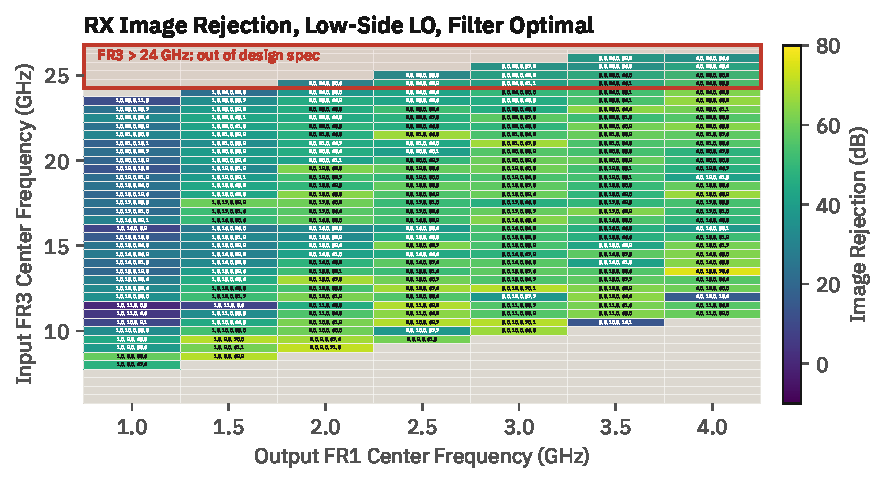
\includegraphics[width=\linewidth]{images/sec11_fig3.pdf}};
    \begin{scope}[x={(img.south east)}, y={(img.north west)}]
      \draw[red!80!black, line width=0.9pt] (\imgOutlierAX,\imgOutlierAY) circle (4.2pt);
      \draw[red!80!black, line width=0.9pt] (\imgOutlierBX,\imgOutlierBY) circle (4.2pt);
      \node[red!80!black, font=\tiny\bfseries, anchor=north] at ({(\imgOutlierAX+\imgOutlierBX)/2},{\imgOutlierAY-0.03}) {See footnote \imgrejoutlierfn};
    \end{scope}
  \end{tikzpicture}
  \captionof{figure}{LO: Low-side. Filter: Optimal. Image rejection (dB) across the full grid.}\label{fig:11-3}
\end{minipage}\hfill
\begin{minipage}[t]{0.46\linewidth}
  \centering
  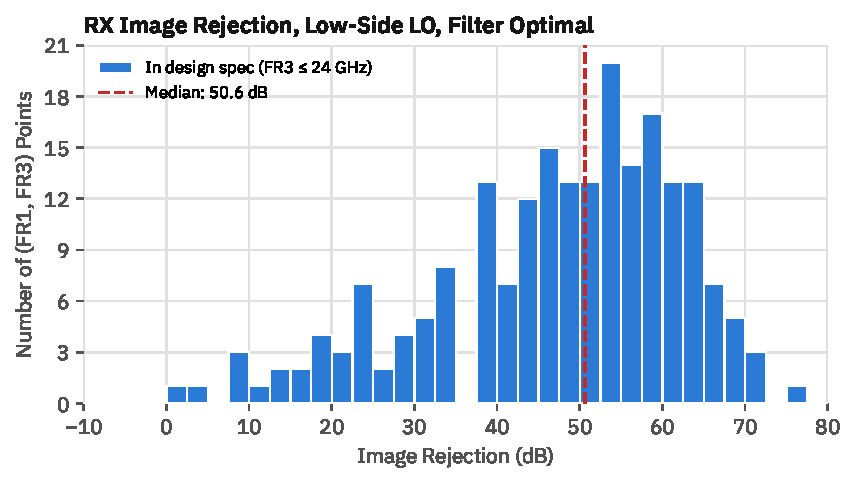
\includegraphics[width=\linewidth]{images/sec11_fig4.pdf}
  \captionof{figure}{LO: Low-side. Filter: Optimal. Distribution of Figure~\ref{fig:11-3}.}\label{fig:11-4}
\end{minipage}
\par\vspace{0.3em}
\figpair{images/sec11_fig5.pdf}{LO: High-side. Filter: Bypassed. Image rejection (dB) across the full grid.}{fig:11-5}%
        {images/sec11_fig6.pdf}{LO: High-side. Filter: Bypassed. Distribution of Figure~\ref{fig:11-5}.}{fig:11-6}
\figpair{images/sec11_fig7.pdf}{LO: High-side. Filter: Optimal. Image rejection (dB) across the full grid.}{fig:11-7}%
        {images/sec11_fig8.pdf}{LO: High-side. Filter: Optimal. Distribution of Figure~\ref{fig:11-7}.}{fig:11-8}
\endgroup

\clearpage
\section{RX-side Noise Figure and Sensitivity}
\label{sec:rx-noise-figure}
\raggedbottom% this section's pages end naturally (no stretched gaps); restored at the end
% Generated by FR3_Characterization/plot_datasheet_nf.py -- do not edit by hand.
\newcommand{\nfLowMin}{5.2}
\newcommand{\nfLowMedian}{12.2}
\newcommand{\nfLowPninety}{16.5}
\newcommand{\nfLowMax}{22.9}
\newcommand{\nfLowCount}{224}
\newcommand{\nfHighMin}{5.6}
\newcommand{\nfHighMedian}{11.0}
\newcommand{\nfHighPninety}{15.8}
\newcommand{\nfHighMax}{20.5}
\newcommand{\nfHighCount}{203}
\newcommand{\nfMedian}{11.5}
\newcommand{\nfCount}{427}
\newcommand{\nfMinMargin}{14}
\newcommand{\nfOosCount}{15}
\newcommand{\nfOosMin}{10.4}
\newcommand{\nfOosMedian}{16.1}
\newcommand{\nfOosMax}{24.1}
\newcommand{\sensCW}{-162.5}
\newcommand{\sensOneM}{-102.5}
\newcommand{\sensFiveM}{-95.5}
\newcommand{\sensTenM}{-92.5}
\newcommand{\sensFiftyM}{-85.5}
\newcommand{\sensHundredM}{-82.5}
\newcommand{\sensFiveHundredM}{-75.5}
\newcommand{\nfStripeLow}{6.0}
\newcommand{\nfStripeHigh}{4.0}


This section first explains what noise figure is, how it sets the receiver's sensitivity, and how it was measured
(Section~\ref{sec:nf-concept}). It then gives the measured noise figure with the ``optimal'' AM3153 filter engaged
(Section~\ref{sec:nf-optimal}), the setting most users will run.

\subsection{Noise Figure: The Concept}
\label{sec:nf-concept}

\textbf{A Motivating Example.} Every receiver adds some noise of its own to whatever it receives. Even with
nothing at all connected to the ``RX-side FR3 RF In'' connector except a 50\,$\Omega$ termination, the termination's
own thermal noise comes in --- about −174\,dBm in every 1\,Hz of bandwidth at room temperature --- and every amplifier, mixer, and filter along the RX chain then adds more on top. The \emph{noise figure} (NF) measures how
much the receiver makes things worse: it is how many dB noisier the output is than it would be if the
receiver were a perfect, noiseless amplifier with the same gain. A receiver with NF~=~0\,dB adds nothing; one
with NF~=~6\,dB puts out four times the noise power a perfect receiver would. A lower NF means weaker signals
can still be heard above the noise.

\textbf{Which noise figure?} The mixer converts noise from \emph{both} RF frequencies that land on the same IF ---
the desired one and its image (see Section~\ref{sec:rx-image-rejection}). The NF in this section counts all of the
noise that reaches the IF output against the gain of the desired signal alone. That is the \emph{single-sideband}
(SSB) noise figure, the one that applies when receiving an ordinary signal that occupies only one side of the
LO.\footnote{Some datasheets quote a \emph{double-sideband} (DSB) NF instead, which credits the receiver for the
gain at both sidebands and therefore comes out up to 3\,dB lower. The SSB figure is the honest one for this unit's
normal use.}

\textbf{From noise figure to sensitivity.} \emph{Sensitivity} is the weakest signal the receiver can use,
and it follows directly from the NF:
\begin{center}
Sensitivity (dBm) = −174 + NF + 10·log\textsubscript{10}(bandwidth in Hz) + required SNR (dB)
\end{center}
The first three terms are the receiver's noise floor, referred to its input, over the signal's bandwidth;
the last is how far above that noise floor the signal has to be for the demodulator to work, which depends on
the modulation and coding, not on this unit. Every dB of NF is therefore a dB of sensitivity.

\textbf{How it's measured.} The unit's NF is found from two separate measurements at exactly the same
settings (same FR1, FR3, LO, and filter), both read at the ``RX-side FR1 IF Out'' connector:\footnote{This is the
``gain method''. It needs no calibrated noise source --- only a spectrum analyzer that is much quieter than
the unit's own output noise. Here the analyzer's own noise floor sat at least \nfMinMargin\,dB below the unit's
output noise at every point; it was measured separately and subtracted from every reading.}
\begin{enumerate}
  \item \textbf{Output noise.} With the RF input terminated in 50\,$\Omega$, measure the noise density at the IF
        output, in dBm/Hz.
  \item \textbf{Gain.} Feed in a weak CW tone of known power (−50\,dBm, well below the point where the chain
        starts to compress) and measure the IF output tone, to get the conversion gain.
\end{enumerate}
Both readings are referred to the unit's connectors: the losses of the cables between the unit and the analyzer
are removed from the output noise as well as from the gain. Then NF = (output noise) − (gain) + 174, all in dB. For example, an output noise of −120\,dBm/Hz with
45\,dB of gain gives NF = −120 − 45 + 174 = 9\,dB. The input tone power was itself measured, at every FR3
frequency, through the same cable used to feed the unit, rather than trusting the signal generator's
nominal setting.\footnote{The generator was within a few tenths of a dB of nominal across 6--26.5\,GHz,
with a few narrow dips of up to 0.7\,dB; the measured value is used throughout.} All readings use 100
power-domain averages.

\textbf{What's plotted.} NF was measured at \nfCount{} (FR1, FR3) combinations: FR1 from 1 to 4\,GHz and FR3
from 6 to 26.5\,GHz, both in 0.5\,GHz steps, for both low-side and high-side LO, wherever the LO falls between
7 and 22.5\,GHz, with the ``optimal'' filter engaged at every point. Grey cells
are combinations that would need the LO outside that range. In the heatmaps, \emph{darker is better} (lower NF),
the same ``darker is better'' sense as the gain figures, and both heatmaps share one colour scale so they can be
compared by eye. FR3 values above the unit's rated 24\,GHz maximum are measured and shown too, inside a red ``out of
design spec'' box. Because NF is a CW measurement, read at a single IF frequency, FR1 = 4\,GHz lies inside the
0.7--4.0\,GHz IF spec (unlike the conversion-gain figures, whose 500\,MHz windows run past it).

\textbf{A note about the 10\,MHz clock comb.} The noise is read 200\,kHz away from each IF frequency, not exactly on
it. The unit's 10\,MHz reference clock leaks a weak comb of spurious tones into the IF output, strongest at
multiples of 20\,MHz (with weaker ones at the odd multiples of 10\,MHz); it comes from the reference clock buffer,
and it sits a few dB to about 12\,dB above the noise floor at the strongest lines.
Reading 200\,kHz away keeps it out of the measurement. In use, it matters only when receiving an extremely weak CW
signal placed exactly on a multiple of 10\,MHz at the IF, where a comb line can sit on top of it; if that happens,
move the IF (or the LO) by a few hundred kHz. For a wideband signal it hardly matters: a 100\,MHz OFDM signal with
1024 subcarriers has only about ten subcarriers on comb lines, which together raise the total in-band noise by well
under 0.1\,dB.

\subsection{Noise Figure: Optimal Filter Engaged}
\label{sec:nf-optimal}

The AM3153 filter is what gives the RX side its image rejection (Section~\ref{sec:rx-image-rejection}), but it sits
after the LNA, so its insertion loss also adds to the noise figure. Here it is engaged at every point in its ``optimal''
setting, the same per-point choice used throughout this datasheet (Section~\ref{sec:sideband-suppression}).

\textbf{With the filter bypassed, the noise figure is lower.} Nothing then sits between the LNA and the mixer, so the
filter's loss no longer adds to the noise. The price is image rejection: a signal at the image frequency then reaches
the IF output almost unattenuated (Section~\ref{sec:rx-image-rejection}). Since most users engage the filter for its
image rejection, only the optimal-filter setting is characterized here. If your incoming FR3 signal is very weak and
nothing is transmitting at its image, bypassing the filter will lower the noise figure.

\textbf{Measurement conditions.} \lmxDriveRule{} (set from the LO frequency). Because the LO is shared, the TX side
was set up exactly as in normal use (its stored LO-leakage calibration applied and its optimal filter engaged), with
both TX-side ports terminated in 50\,\textohm. The unit was measured hot: no fan, LMX2820 die at
\condRxNfMinC--\condRxNfMaxC\textdegree C.

\textbf{Results.} Across all points up to the rated 24\,GHz, the median NF is \nfMedian\,dB. Over that same
range, with low-side LO the NF runs from \nfLowMin{} to \nfLowMax\,dB (median \nfLowMedian\,dB, and 90\% of
points at or below \nfLowPninety\,dB); with high-side LO it runs from \nfHighMin{} to \nfHighMax\,dB (median
\nfHighMedian\,dB, 90\% at or below \nfHighPninety\,dB) (Figures~\ref{fig:12-1}--\ref{fig:12-4}).
Above the rated 24\,GHz the unit still works, just out of design spec: the \nfOosCount{} points measured there (all
with low-side LO, boxed in red in Figure~\ref{fig:12-1}; the histograms count only the points within the design spec)
have an NF from \nfOosMin{} to \nfOosMax\,dB (median \nfOosMedian\,dB).

\textbf{Sensitivity.} At the median NF of \nfMedian\,dB, the input-referred noise floor (required SNR = 0\,dB) is:
\par\medskip\noindent\begin{minipage}{\linewidth}% caption and table stay on one page
\begin{center}
\captionof{table}{Input-referred noise floor at the median NF, optimal filter engaged.}\label{tab:nf-floor-optimal}
\vspace{0.4em}
\begin{tabular}{lc}
\toprule
Signal bandwidth & Noise floor at the RF input \\
\midrule
CW tone\textsuperscript{*} & \sensCW\,dBm/Hz \\
1\,MHz & \sensOneM\,dBm \\
5\,MHz & \sensFiveM\,dBm \\
10\,MHz & \sensTenM\,dBm \\
50\,MHz & \sensFiftyM\,dBm \\
100\,MHz & \sensHundredM\,dBm \\
500\,MHz & \sensFiveHundredM\,dBm \\
\bottomrule
\multicolumn{2}{l}{\footnotesize\textsuperscript{*}Per 1\,Hz of detection bandwidth (see below).}
\end{tabular}
\end{center}
\end{minipage}\par
Add the required SNR to get the sensitivity. For example, a signal needing 10\,dB of SNR in 100\,MHz has a
sensitivity 10\,dB above the 100\,MHz noise floor in the table. A CW tone has no bandwidth of its own, so its
noise floor depends on the bandwidth it is detected in: add 10·log\textsubscript{10} of that bandwidth in Hz to the CW row, e.g.\ +40\,dB for 10\,kHz.

\textbf{Where the NF is worst, and how to avoid it.} The clearest feature in both heatmaps is a stripe of
higher NF wherever the LO sits at 14.0 or 14.5\,GHz: there the median NF is about \nfStripeLow\,dB (low-side LO)
and \nfStripeHigh\,dB (high-side LO) worse than with the LO at the neighbouring 13--13.5 and 15--15.5\,GHz, at every
FR1. Because it follows the LO frequency rather than the RF frequency, it shows up as a diagonal stripe in the
low-side heatmap (FR3 = LO + FR1) and as the mirror diagonal in the high-side one (FR3 = LO − FR1). If your FR3 and
FR1 put the LO at 14 to 14.5\,GHz, switching to the other LO side moves the LO by twice the FR1 frequency, well
clear of that stripe, usually for a much better NF. None of this matters unless the incoming FR3 signal is weak
enough to sit close to the receiver's noise floor: a stronger signal stays far above the added noise either way.

\medskip
\figpair{images/sec12_fig1.pdf}{Noise figure, low-side LO: full measured (FR1, FR3) grid, optimal filter.
Zoom in to read each cell's exact values, printed as (FR1, FR3, noise figure), with FR1 and FR3 in GHz and the
noise figure in dB.}{fig:12-1}%
        {images/sec12_fig2.pdf}{LO: Low-side. Filter: Optimal. Distribution of Figure~\ref{fig:12-1}, points within the design spec.}{fig:12-2}
\figpair{images/sec12_fig3.pdf}{Noise figure, high-side LO: full measured (FR1, FR3) grid, optimal filter.
Zoom in to read each cell's exact values, printed as (FR1, FR3, noise figure), with FR1 and FR3 in GHz and the
noise figure in dB.}{fig:12-3}%
        {images/sec12_fig4.pdf}{LO: High-side. Filter: Optimal. Distribution of Figure~\ref{fig:12-3}, points within the design spec.}{fig:12-4}
\clearpage
\flushbottom

\clearpage
\section{Phase Noise}
\label{sec:phase-noise}
\raggedbottom% this section's pages end naturally (flushbottom spread large gaps through the step list); restored at the end
% Generated by FR3_Characterization/plot_datasheet_pn.py -- do not edit by hand.
\newcommand{\pnLoLow}{8}
\newcommand{\pnLoHigh}{22}
\newcommand{\pnScaleExpected}{8.8}
\newcommand{\pnScaleMin}{8.0}
\newcommand{\pnScaleMax}{8.9}
\newcommand{\pnRmsLow}{0.82}
\newcommand{\pnRmsHigh}{2.13}
\newcommand{\pnCount}{8}
\newcommand{\pnUnwantedMin}{20}
\newcommand{\pnUnwantedMax}{65}
\newcommand{\pnOctoFig}{images/sec14_fig9.pdf}
\newcommand{\pnOctoRms}{0.24}
\newcommand{\pnBoardTenRms}{1.02}
\newcommand{\pnOctoRmsRatio}{4.3}
\newcommand{\pnOctoGainMin}{12}
\newcommand{\pnOctoGainMax}{21}


\textbf{A Motivating Example.} An ideal LO would be a perfect sine wave: all of its power at exactly one
frequency, a single infinitely thin line on a spectrum analyzer. A real LO wobbles slightly in phase from moment
to moment, and that wobble spreads a little of its power out into ``skirts'' on either side of the carrier.
\emph{Phase noise} measures how much power sits in those skirts, at a given distance (the \emph{offset}) from
the carrier, in a 1\,Hz bandwidth, relative to the carrier itself --- hence the unit dBc/Hz. For example,
−90\,dBc/Hz at a 100\,kHz offset means that 100\,kHz away from the carrier, each 1\,Hz slice holds a
billionth of the carrier's power. Lower is better.

\textbf{Why it matters.} Every signal the unit up- or down-converts is multiplied by the LO, so the LO's
skirts are copied onto every signal that passes through. On the transmit side they blur each transmitted
subcarrier into its neighbors and smear the constellation of a modulated signal. On the receive side a strong
signal on a nearby channel, mixed with the LO's skirts, lands on top of a weak wanted signal (``reciprocal
mixing''). A single summary figure is the \emph{RMS phase error}: the total phase wobble, in degrees, integrated
over all the measured offsets. Higher-order modulations (64-QAM and above) need it to be a fraction of a
degree to a few degrees, depending on the signal.

\textbf{How it's measured.} The LO is not brought out to a connector of its own, so it is measured through the
small amount of it that leaks out of the ``TX-side FR3 RF Out'' connector, with nothing connected to the
``TX-side FR1 IF In'' connector except a 50\,$\Omega$ termination. The leakage is a copy of the LO, so its
phase noise is the LO's phase noise. Three steps make the measurement clean:\footnote{Measured with a Keysight
UXA signal analyzer and its Phase Noise application (log-plot measurement, 100\,Hz to 1\,MHz offset, signal
tracking on, 10 averages). The analyzer's own phase noise is well below the unit's at every offset shown.}
\begingroup\setlength{\leftmargini}{2.2em}\setlength{\topsep}{0.4em}% indent slightly; fixed (non-stretching) spacing
\begin{enumerate}\setlength{\itemsep}{0.4em}\setlength{\parsep}{0pt}
  \item \textbf{A fixed, moderate carrier level.} The I/Q DC bias described in Section~\ref{sec:lo-suppression}
        is moved slightly away from its LO-null point until the leakage at the ``TX-side FR3 RF Out'' connector
        is exactly 0\,dBm --- strong enough to measure well, and well below the level at which the TX chain
        starts to compress.
  \item \textbf{A filter that passes only the LO.} The LMX2820 synthesizer produces one other tone besides the
        LO. Up to 11.3\,GHz its oscillator drives the output directly, so its second harmonic (twice the LO
        frequency) is present; above 11.3\,GHz the output is the oscillator's frequency doubled, so the
        oscillator's own frequency (half the LO frequency) is present. At each LO frequency the AM3153 filter
        is set to pass the LO and block that other tone, so the analyzer measures the LO and nothing
        else.\footnote{The filter is chosen with the same two-step rule as the ``optimal'' filter of
        Section~\ref{sec:sideband-suppression}: keep the LO within 3\,dB of the best available, then block the
        unwanted tone as much as possible. With the filter in place, the unwanted tone sat between
        \pnUnwantedMin{} and \pnUnwantedMax\,dB below the LO at the ``TX-side FR3 RF Out'' connector.}
  \item \textbf{Time to settle.} After each retune, the synthesizer is given 5\,s to settle fully before the
        measurement starts.
\end{enumerate}
\endgroup

\textbf{What's plotted.} \pnCount{} LO frequencies, from \pnLoLow{} to \pnLoHigh\,GHz in 2\,GHz steps, each in
its own figure: phase noise against offset from the carrier, from 100\,Hz to 1\,MHz. Every curve is the average of
10 complete measurements. Each figure shows that average twice: the thin line is the average as measured
(unsmoothed), and the thick line is the analyzer's lightly smoothed version of it, which makes the trend easier
to read. The figures follow on the next page; the values marked at every decade offset, the table after them, and
the RMS phase error all come from the smoothed curve.\footnote{All measurements use the unit's own
10\,MHz TCXO and internal LMX2820 synthesizer, the default configuration.}

\clearpage
% Page of its own: all eight per-LO figures (user layout, 2026-10-04). Section-local, slightly narrower figpair
% so four rows fit on one page; scoped so the document-wide \figpair is unchanged.
\begingroup
\renewcommand{\figpair}[6]{%
  \noindent
  \begin{minipage}[t]{0.44\linewidth}\centering\includegraphics[width=\linewidth]{#1}\captionof{figure}{#2}\label{#3}\end{minipage}\hfill
  \begin{minipage}[t]{0.44\linewidth}\centering\includegraphics[width=\linewidth]{#4}\captionof{figure}{#5}\label{#6}\end{minipage}
  \par\vspace{0.6em}
}
\figpair{images/sec14_fig1.pdf}{LO = 8\,GHz.}{fig:14-1}%
        {images/sec14_fig2.pdf}{LO = 10\,GHz.}{fig:14-2}
\figpair{images/sec14_fig3.pdf}{LO = 12\,GHz.}{fig:14-3}%
        {images/sec14_fig4.pdf}{LO = 14\,GHz.}{fig:14-4}
\figpair{images/sec14_fig5.pdf}{LO = 16\,GHz.}{fig:14-5}%
        {images/sec14_fig6.pdf}{LO = 18\,GHz.}{fig:14-6}
\figpair{images/sec14_fig7.pdf}{LO = 20\,GHz.}{fig:14-7}%
        {images/sec14_fig8.pdf}{LO = 22\,GHz.}{fig:14-8}
\endgroup
\clearpage

\par\medskip\noindent\begin{minipage}{\linewidth}% caption and table stay on one page
\begin{center}
\captionof{table}{Phase noise of the internal LO at each decade offset, read from the smoothed curves of
Figures~\ref{fig:14-1}--\ref{fig:14-8}, and the RMS phase error integrated from 100\,Hz to 1\,MHz.}\label{tab:14-1}
\vspace{0.4em}
% Generated by FR3_Characterization/plot_datasheet_pn.py -- do not edit by hand.
\begin{tabular}{|l|ccccc|c|}
\hline
\textbf{LO} & \textbf{100\,Hz} & \textbf{1\,kHz} & \textbf{10\,kHz} & \textbf{100\,kHz} & \textbf{1\,MHz} & \textbf{RMS phase error} \\
 & \multicolumn{5}{c|}{(dBc/Hz)} & (degrees) \\
\hline
8\,GHz & −63.9 & −85.4 & −88.4 & −97.3 & −123.7 & 0.82 \\
10\,GHz & −62.3 & −83.3 & −86.5 & −95.1 & −122.1 & 1.02 \\
12\,GHz & −60.6 & −81.8 & −85.0 & −93.2 & −119.3 & 1.25 \\
14\,GHz & −58.4 & −80.9 & −83.8 & −92.0 & −118.2 & 1.46 \\
16\,GHz & −58.0 & −79.2 & −82.5 & −91.1 & −118.5 & 1.63 \\
18\,GHz & −57.4 & −78.1 & −82.0 & −90.2 & −116.9 & 1.80 \\
20\,GHz & −55.2 & −77.1 & −80.2 & −89.2 & −116.0 & 2.06 \\
22\,GHz & −55.4 & −76.5 & −80.2 & −89.3 & −117.2 & 2.13 \\
\hline
\end{tabular}

\end{center}
\end{minipage}\par

\textbf{Reading the curves.} Three features are worth noticing. First, every curve has the same shape, and
the whole curve moves up as the LO frequency goes up: from \pnLoLow{} to \pnLoHigh\,GHz the phase noise rises
by \pnScaleMin{} to \pnScaleMax\,dB at every offset. This is expected: multiplying a frequency by N multiplies its
phase wobble by N too, which raises phase noise by 20·log\textsubscript{10}(N), and
20·log\textsubscript{10}(\pnLoHigh/\pnLoLow) = \pnScaleExpected\,dB. The same rule sets the close-in part of each
curve: the LO is locked to a 10\,MHz reference, so close to the carrier it inherits that reference's phase noise
multiplied up by the ratio of the two frequencies --- at 10\,GHz, a factor of 1000, or +60\,dB. Second, beyond
roughly 200\,kHz every curve falls steeply: that is where the synthesizer's control loop stops following the
reference and the curve takes on the oscillator's own, falling, phase noise. Third, the RMS phase error grows
with frequency for the same reason, from \pnRmsLow\textdegree{} at \pnLoLow\,GHz to \pnRmsHigh\textdegree{} at
\pnLoHigh\,GHz. In practice: for the lowest phase noise, use the lowest LO frequency your FR1 and FR3 choices
allow.

\textbf{A cleaner LO: the OctoLO.} When phase noise matters most, the unit's own synthesizer can be bypassed
entirely: selecting External LO (Section~\ref{sec:hw-clock-lo}) routes a signal from the ``LO In'' connector to
both mixers instead. Figure~\ref{fig:14-9} compares the internal LO at 10\,GHz with the Pi-Radio OctoLO tuned to
the same frequency, measured with identical analyzer settings.\footnote{The OctoLO was connected directly to the
analyzer, so this figure shows the source itself. Near 1\,kHz its phase noise comes close to the analyzer's own,
so its true value there may be slightly lower still.} From 100\,Hz to 100\,kHz the OctoLO is \pnOctoGainMin{} to
\pnOctoGainMax\,dB quieter, and its RMS phase error is \pnOctoRms\textdegree{} instead of
\pnBoardTenRms\textdegree{} --- about \pnOctoRmsRatio{} times lower.

\figrow{\pnOctoFig}{LO = 10\,GHz: the internal LO compared with the Pi-Radio OctoLO. Thick lines are smoothed,
thin lines unsmoothed; both are the average of 10 measurements.}{fig:14-9}

\clearpage % start this discussion on a fresh page (it otherwise left a single line at the foot of page 38)
\textbf{What RMS phase error means for a modulation.} Picture a constellation diagram. Every symbol the
receiver gets is a dot, and the receiver decides which symbol was sent by checking which ideal point the dot is
closest to. Phase noise makes the whole constellation twist back and forth around its center, like a wheel being
jiggled: every dot slides sideways along a circle, and the RMS phase error is how far, in degrees, that twist
typically goes. A twist only causes an error once it carries a dot closer to a neighboring point than to its
own. BPSK has just two points, on opposite sides of the circle, so it shrugs off large twists; QPSK has four, a
quarter turn apart; 16-QAM, 64-QAM, and 256-QAM pack ever more points into the same space, with their outer
points crowded closest together around the circle, so each step up tolerates less twist. Wireless standards
such as 5G NR capture this by limiting how far, on average, the received dots may stray from their ideal positions --- the
error vector magnitude (EVM), a percentage of the signal's size --- with a tighter limit for each denser
modulation. Translating each limit into degrees of twist gives the most RMS phase error each modulation could
tolerate if phase noise were the \emph{only} thing disturbing it:
\par\medskip\noindent\begin{minipage}{\linewidth}% caption and table stay on one page
\begin{center}
\captionof{table}{EVM limit of each modulation, and the RMS phase error it would allow if phase noise were the only impairment.}\label{tab:evm-phase}
\vspace{0.4em}
\begin{tabular}{lcc}
\toprule
\textbf{Modulation} & \textbf{EVM limit} & \textbf{RMS phase error, if it were the only impairment} \\
\midrule
QPSK & 17.5\% & about 10\textdegree \\
16-QAM & 12.5\% & about 7\textdegree \\
64-QAM & 8\% & about 4.6\textdegree \\
256-QAM & 3.5\% & about 2.0\textdegree \\
\bottomrule
\end{tabular}
\end{center}
\end{minipage}\par
In a real link, phase noise must share that budget with everything else (thermal noise, nonlinearity, I/Q
imbalance), and both ends of the link contribute their own LO's phase noise, so a comfortable design keeps phase
noise to well under half of these limits. Against that yardstick, the internal LO (\pnRmsLow\textdegree{} at
\pnLoLow\,GHz up to \pnRmsHigh\textdegree{} at \pnLoHigh\,GHz) supports QPSK to 64-QAM comfortably at every LO
frequency, while 256-QAM is within reach only at the lower LO frequencies and becomes tight toward the top of the
range. The OctoLO, at \pnOctoRms\textdegree{}, leaves ample margin even for 256-QAM.\footnote{The RMS phase error
here is integrated from 100\,Hz to 1\,MHz offset. OFDM receivers track and remove much of the slow, close-in phase
wobble, which makes the close-in part matter less; phase noise beyond 1\,MHz, not included here, adds a little.
The comparison above is a guide to where each LO's limits lie, not a link budget.}

\textbf{An Acknowledgement.} Pi-Radio does not own phase noise measurement equipment. The measurements in this
section were made for us by Prof.\ Hamed Rahmani at New York University, on his lab's Keysight N9042B UXA signal
analyzer. We are grateful for his help. The analyzer's phase noise measurement software was a donation from
Keysight, and we are grateful to Keysight too.

\clearpage
\flushbottom

\clearpage
\section{Tips for Correct Usage}
\label{sec:tips}

Using the Pi-Radio FR3-1ch is easy: pick your FR1 and FR3 center frequencies (and, on TX, the sideband), and it just
works --- the unit works out the LO frequency, switch states, and LO-null bias on its own. A few corner cases are
worth knowing about, though, because in them your choice of configuration makes a real difference. Each is
described below, with what to do about it and where in this datasheet it is measured.

\textbf{Before going over the air, check the regulations.} Before transmitting from an antenna, make sure your
signal meets every regulation that applies where you operate it --- including the permitted frequencies,
bandwidth, transmit power, and emissions outside your channel --- and that you hold any license it requires. Staying
within the rules is the operator's responsibility, and Pi-Radio is not responsible for any regulatory violation.

\textbf{Protect the unit from static (ESD).} The unit is static-sensitive: some of the parts inside it can be damaged by an
electrostatic discharge of under 150\,V (Table~\ref{tab:summary-absmax}), far less than a person can build up just
by walking across a room, and well below what you can feel. The damage is not always obvious: a part can keep working
but with degraded performance. We strongly recommend using the system in its box, as shipped: there is then never a
reason to touch the board itself, and the connectors are the only way a discharge can reach it. So take care each time
you connect something. Work on a grounded anti-static mat, wearing a grounded wrist strap; if you have neither, at
least touch grounded metal first. Before connecting any cable to any connector, touch the cable's outer shell to
ground, so that any charge it has picked up drains away there rather than through the unit; this matters most for
cables from an antenna or from other equipment.

\textbf{Keep the input within the linear range.} Each chain is linear only up to its input P1dB, which depends on
the (FR1, FR3) combination: Sections~\ref{sec:compression-upper} and \ref{sec:compression-lower} give it for TX,
Sections~\ref{sec:rx-compression-lowside} and \ref{sec:rx-compression-highside} for RX, and the Key Specifications
page summarizes the range. Drive the unit past it and the signal distorts. Separately, never exceed the absolute
maximum input levels on the Key Specifications page.

\textbf{The lower sideband (TX) and high-side LO (RX) mirror the spectrum.} With the TX lower sideband, or equivalently
a high-side LO on RX, the signal's spectrum comes out flipped: a feature at the top of the FR1 band lands at the
bottom of the FR3 band, and vice versa (Section~\ref{sec:hardware-primer}). Most receivers can undo this (for example
by conjugating the baseband samples), but your system has to know about it.

\textbf{When to engage the AM3153 filter.} The filter is what suppresses the unwanted sideband on TX
(Section~\ref{sec:sideband-suppression}) and the image on RX (Section~\ref{sec:rx-image-rejection}); with it
bypassed, both are poor. Its cost is some conversion gain, and on RX a higher noise figure
(Section~\ref{sec:rx-noise-figure}). Engage it whenever the unwanted sideband or image matters; bypass it only when
you need the lowest possible RX noise figure and know that nothing is transmitting in the image band.

\textbf{An interferer sits on the RX image.} The RX receives both LO\,+\,FR1 and LO\,$-$\,FR1, and one of them is
the image (Section~\ref{sec:rx-image-rejection}). If a known interferer sits on the image, switch to the other LO
side: the LO, and with it the image, moves by twice the FR1 frequency, away from the interferer.

\textbf{Image rejection is weakest at low FR1.} At low FR1 the wanted signal and its image are close together, so
the filter has a harder time separating them. If image rejection matters, use a higher FR1 for the same FR3
(Section~\ref{sec:rx-image-rejection}).

\textbf{Avoid an LO at exactly twice the FR1.} When the LO is exactly twice the FR1 frequency, a spurious mixing
product lands on the wanted IF and RX image rejection drops sharply (Section~\ref{sec:rx-image-rejection}). Avoid
that exact configuration, or choose the sideband so that the LO stays at 9\,GHz or above.

\textbf{RX noise figure is worse with the LO at 14--14.5\,GHz.} With the LO at 14.0 or 14.5\,GHz, the RX noise figure
is typically 4 to 5\,dB worse than at neighboring LO frequencies (Section~\ref{sec:rx-noise-figure}). This only
matters for weak signals near the noise floor; if that is your case, switch to the other LO side, which moves the
LO by twice the FR1 frequency.

\textbf{Weak CW signals on a 10\,MHz grid.} The RX IF output carries a weak comb of tones at multiples of 10\,MHz
(Section~\ref{sec:rx-noise-figure}). It matters only for an extremely weak CW signal that lands exactly on that grid;
if yours does, move the IF (or the LO) by a few hundred kHz.

\keepnext{5\baselineskip}% the whole paragraph moves to the next page rather than split
\textbf{Phase noise rises with the LO frequency.} The LO's phase noise grows with its frequency
(Section~\ref{sec:phase-noise}). For the highest-order modulations (256-QAM), choose the FR1 and sideband that put
the LO as low as possible, or use an external low-noise LO such as the Pi-Radio OctoLO via the ``LO In'' connector.

\textbf{LO suppression depends on temperature.} The LO-null bias is calibrated at two temperatures and interpolated at
runtime from the LMX2820's die temperature (Section~\ref{sec:lo-suppression}). LO suppression is best once the unit
has reached a steady temperature after power-up, and with the LMX die between the two calibrated temperatures. Keep
the LMX die below 100\,\textdegree C in any case.

\textbf{Stay inside the design range.} The unit is rated for FR3 up to 24\,GHz and FR1 from 0.7 to 4.0\,GHz.
Measurements beyond these limits are shown throughout this datasheet, boxed in red, and the unit still works there,
but its performance outside them is not guaranteed.

\clearpage
\appendix
\section{Using the Pi-Radio GUI}
\label{sec:gui}
\raggedbottom% this appendix's pages end naturally (no stretched paragraph gaps)
% generated by tools/crop_gui_screenshots.py -- do not edit
% callout positions on images/gui_shot_<section>.png: fractions, x from the left, y from the bottom
\newcommand{\guiCOOneX}{0.0142}
\newcommand{\guiCOOneY}{0.9083}
\newcommand{\guiCOTwoX}{0.5480}
\newcommand{\guiCOTwoY}{0.7114}
\newcommand{\guiCOThreeX}{0.1368}
\newcommand{\guiCOThreeY}{0.6895}
\newcommand{\guiCOFourX}{0.0231}
\newcommand{\guiCOFourY}{0.4913}
\newcommand{\guiCOFiveX}{0.0231}
\newcommand{\guiCOFiveY}{0.2303}
\newcommand{\guiCOSixX}{0.0486}
\newcommand{\guiCOSixY}{0.6011}
\newcommand{\guiCOSevenX}{0.0368}
\newcommand{\guiCOSevenY}{0.1617}
\newcommand{\guiCOEightX}{0.0368}
\newcommand{\guiCOEightY}{0.3172}

% \guishot{image}{width}{callouts as n/X/Y,...}: a section screenshot with red numbered callouts. A callout whose control
% sits at the left edge goes in the margin just left of the image; otherwise it sits just left of the control.
\newcommand{\guishot}[3]{%
  \begin{tikzpicture}
  \node[anchor=south west, inner sep=0] (img) at (0,0) {\includegraphics[width=#2]{#1}};
  \begin{scope}[x={(img.south east)}, y={(img.north west)}]
  \foreach \n/\X/\Y in {#3}{%
    \pgfmathsetmacro{\cx}{\X < 0.1 ? -0.022 : \X - 0.018}%
    \node[circle, fill=red!80!black, text=white, font=\scriptsize\bfseries, inner sep=1pt, minimum size=10pt]
      at (\cx,\Y) {\n};}
  \end{scope}
  \end{tikzpicture}}

The Pi-Radio GUI is the easiest way to set up the unit. It talks to the unit over the same USB-serial commands listed in
Appendix~\ref{sec:commands}, so anything the GUI can do, a script can do too. This appendix describes GUI version~1.4.1,
for units running firmware~1.4.1. The images are screenshots of the GUI controlling a unit set up for an FR1 of 1\,GHz,
an FR3 of 9\,GHz, and the upper sideband; the red numbers are explained below each image.

\textbf{Starting.} Start the GUI and plug the unit in, in either order. The GUI finds each connected unit by itself and
opens one tab per unit; the line at the top of the tab shows the hardware revision, the unit's serial number, its serial
port, and whether it is connected. Only one program can use a unit's serial port at a time: before using a terminal or a
script, close the GUI or press its \textbf{Disconnect} button, and close the other program before reconnecting the GUI.
Each tab has four sections, top to bottom: the Configuration Helper, Clocking and LO, TX Settings, and RX Settings. Click
a section's title to fold it away.

\par\medskip\noindent\begin{minipage}{\linewidth}\centering
\guishot{images/gui_shot_helper.png}{0.9\linewidth}{1/\guiCOOneX/\guiCOOneY, 2/\guiCOTwoX/\guiCOTwoY}
\captionof{figure}{The Configuration Helper.}\label{fig:gui-helper}
\end{minipage}\par
\begin{enumerate}
\setlength{\itemsep}{2pt}
\item \textbf{FR1, FR3, signal bandwidth, and sideband.} Enter what you want; the GUI works out the LO frequency
  (FR3\,$-$\,FR1 for the upper sideband, FR3\,+\,FR1 for the lower), tunes the synthesizer, and sets the sideband
  switch. If that LO is out of range, it says so, keeps the last valid setting, and suggests trying the other sideband.
\item \textbf{The suggested filter.} The graph shows where the wanted signal (green), its image (red), and the LO
  (black) fall, against the measured response of the filter the GUI suggests for these frequencies (blue). This is the
  ``optimal'' filter used throughout this datasheet. The line under the graph gives an estimate of the image rejection
  it buys, not a measurement (Sections~\ref{sec:sideband-suppression} and~\ref{sec:rx-image-rejection}).
\end{enumerate}

\par\medskip\noindent\begin{minipage}{\linewidth}\centering
\guishot{images/gui_shot_clocking.png}{0.9\linewidth}{3/\guiCOThreeX/\guiCOThreeY, 4/\guiCOFourX/\guiCOFourY,
  5/\guiCOFiveX/\guiCOFiveY}
\captionof{figure}{Clocking and LO.}\label{fig:gui-clocking}
\end{minipage}\par
\begin{enumerate}
\setcounter{enumi}{2}
\setlength{\itemsep}{2pt}
\item \textbf{LO drive.} Leave it on \textbf{Automatic}: the unit then sets the synthesizer's drive from the LO
  frequency, as in every measurement in this datasheet. Unticking it lets you choose a fixed drive level.
\item \textbf{Lock status and temperature.} The synthesizer should read \textbf{LOCKED} when the internal synthesizer (VCO/PLL) is
  engaged. Keep its die temperature
  below 100\,\textdegree C (Section~\ref{sec:summary}).
\item \textbf{Clock and LO source.} Internal or external, for the 10\,MHz reference and for the LO. With an external
  LO, the GUI shows the frequency to feed into the ``LO In'' connector, and the unit switches its internal reference
  off and pauses the automatic LO suppression (item~6).
\end{enumerate}

\par\medskip\noindent\begin{minipage}{\linewidth}\centering
\guishot{images/gui_shot_tx.png}{0.9\linewidth}{6/\guiCOSixX/\guiCOSixY, 7/\guiCOSevenX/\guiCOSevenY}
\captionof{figure}{TX Settings.}\label{fig:gui-tx}
\end{minipage}\par
\begin{enumerate}
\setcounter{enumi}{5}
\setlength{\itemsep}{2pt}
\item \textbf{LO suppression.} Leave \textbf{Automatic LO suppression} on: the unit applies its own factory
  calibration (Section~\ref{sec:lo-suppression}), updated every 2\,seconds as it warms up. The line below says what was
  applied and for which temperature, and the grey line which calibration is stored in the unit.
\item \textbf{TX filter.} With \textbf{Use the Configuration Helper's suggested filter} ticked, the TX filter follows
  the suggestion (item~2). Untick it to choose a filter yourself. The line below shows the filter in use.
\end{enumerate}

\par\medskip\noindent\begin{minipage}{\linewidth}\centering
\guishot{images/gui_shot_rx.png}{0.9\linewidth}{8/\guiCOEightX/\guiCOEightY}
\captionof{figure}{RX Settings.}\label{fig:gui-rx}
\end{minipage}\par
\begin{enumerate}
\setcounter{enumi}{7}
\item \textbf{RX filter.} The same, for the RX side, where the filter is what rejects the image
  (Section~\ref{sec:rx-image-rejection}).
\end{enumerate}

\textbf{To reproduce this datasheet's conditions.} Use the internal clock and LO (item~5), leave the LO drive and the LO
suppression on automatic (items~3 and~6), and leave both filters on the suggested filter (items~7 and~8). The
measurements were made with the unit warm --- the synthesizer at about 70--85\,\textdegree C --- which is
also how it runs after a while in normal use.

\textbf{Messages to look out for.} Two states are shown in colour, because they change what the unit does:
\par\medskip\noindent
\begin{minipage}[t]{0.48\linewidth}
\vspace{0pt}
\centering
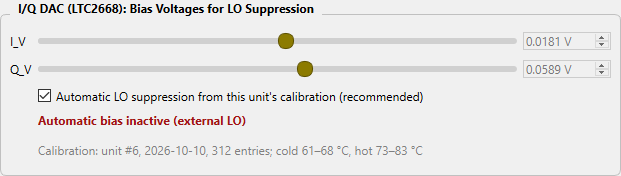
\includegraphics[width=\linewidth]{images/gui_lo_suppr_extlo.png}
\captionof{figure}{External LO selected: the automatic LO suppression is paused (red). The last bias stays applied,
and it is only correct for the frequency it was computed for.}\label{fig:gui-extlo}
\end{minipage}\hfill
\begin{minipage}[t]{0.48\linewidth}
\vspace{0pt}
\centering
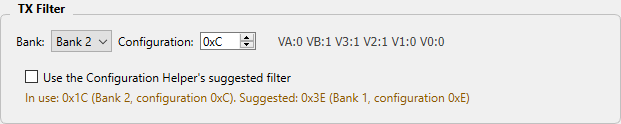
\includegraphics[width=\linewidth]{images/gui_tx_filter_manual.png}
\captionof{figure}{TX filter chosen by hand: the note shows the filter in use and, in amber, the one the Configuration
Helper suggests for the current frequencies.}\label{fig:gui-manual-filter}
\end{minipage}\par
\medskip

\textbf{Nulling the LO yourself.} For the deepest LO suppression in one particular configuration, follow the search in
Section~\ref{sec:lo-suppression}: untick \textbf{Automatic LO suppression} (item~6), then move the I\_V and Q\_V
sliders while watching the LO leakage at the ``TX-side FR3 RF Out'' connector on a spectrum analyzer. Your values stay
applied until you tick the box again, which goes back to the unit's own calibration.

\textbf{Settings the GUI keeps on your computer.} The unit itself remembers every setting it is given (see
Appendix~\ref{sec:commands}). The GUI also remembers, per unit and on the computer it runs on, the FR1, FR3, and signal
bandwidth last entered in the Configuration Helper. If the unit was last set up from another computer, the GUI warns
that these do not match the unit's LO frequency; enter the right values before changing anything else.
\flushbottom

\clearpage
\section{Command Reference}
\label{sec:commands}
\raggedbottom% this appendix's pages end naturally (no stretched paragraph gaps)

Everything the unit does can be controlled over its USB-C connection with plain-text commands --- this is exactly
what the Pi-Radio GUI uses, so anything the GUI can do, a script can do too (Section~\ref{sec:hw-digital}). This
appendix lists every command of firmware version 1.4.1.

\textbf{Connecting.} The unit appears on the computer as a USB virtual serial port (a COM port on Windows,
\texttt{/dev/ttyACM}\textit{n} on Linux, \texttt{/dev/tty.usbmodem}\textit{n} on macOS). The baud-rate setting
does not matter. Any serial terminal (for example PuTTY) or any language with a serial library will do.

\textbf{How commands work.} Each command is one line of text, ended with a carriage return, a line feed, or both.
Commands are not case-sensitive and may be up to 63 characters long. The unit echoes every character as it is
typed, followed by a new line, and then sends exactly one response line: the requested value for a query, or
\texttt{OK} when a setting was applied. A value out of range returns \texttt{ERR}, and an unrecognized command
returns \texttt{ERR:[}\textit{command}\texttt{]len=}\textit{n}, echoing what the unit received. In a terminal, the
up and down arrow keys recall earlier commands. For example:
\par\medskip\noindent\begin{minipage}{\linewidth}% caption and table stay on one page
\begin{center}
\captionof{table}{An example terminal session.}\label{tab:cmd-example}
\vspace{0.4em}
\footnotesize
\begin{tabular}{ll}
\textit{You type} & \textit{The unit replies} \\
\hline
\texttt{*IDN?} & \texttt{FR3 1CH REV1.4,STM32H573VIT6,FW1.4.1} \\
\texttt{LMX TUNE 12000000000} & \texttt{OK} \\
\texttt{LMX LOCK?} & \texttt{LOCKED} \\
\texttt{LMX TEMP?} & \texttt{83.1} \\
\end{tabular}
\end{center}
\end{minipage}\par

\textbf{Settings are remembered.} Every setting marked ``saved'' below is stored in the unit's flash memory, so the
unit powers up in the state it was last left in. For long automated sweeps, \texttt{SET PERSIST OFF} suspends these
flash writes (sparing the flash thousands of writes), and \texttt{SET PERSIST ON} resumes them and saves the current
state once. \texttt{SET PERSIST OFF} lasts only until the next power-up.

\textbf{The unit works in raw values.} The firmware has no notion of FR1, FR3, or sideband: it only sets an LO
frequency, switch states, filter bytes, and bias voltages. Working out those values from an (FR1, FR3, sideband)
choice --- for example LO\,=\,FR3\,$-$\,FR1 and \texttt{SET IQ THRU} for the upper sideband
(Section~\ref{sec:hardware-primer}) --- is done by the host, which the Pi-Radio GUI does for you. Two things the
unit does set by itself, from the LO frequency: the synthesizer's drive level, and the TX LO-null bias voltages from
its own stored calibration (Section~\ref{sec:lo-suppression}). Both are on by default, and both can be switched to
manual.

\begingroup
\footnotesize
\renewcommand{\arraystretch}{1.15}
\newcommand{\cmdtab}[2]{%
  \par\medskip\noindent\begin{minipage}{\linewidth}% caption and table stay on one page
  \begin{center}
  \captionof{table}{Commands: #1.}
  \vspace{0.4em}
  \begin{tabularx}{\linewidth}{|>{\raggedright\arraybackslash}p{0.27\linewidth}|X|>{\raggedright\arraybackslash}p{0.2\linewidth}|}
  \hline
  \textbf{Command} & \textbf{What it does} & \textbf{Response} \\
  \hline
  #2
  \hline
  \end{tabularx}
  \end{center}
  \end{minipage}\par}

\cmdtab{Identification and settings storage}{%
\texttt{*IDN?} & Identifies the unit: name, PCB revision, microcontroller, and firmware version. &
  e.g.\ \texttt{FR3 1CH REV1.4,} \texttt{STM32H573VIT6,FW1.4.1} \\
\texttt{GET BOARD SERIAL} & The unit's factory-programmed serial number; identifies a physical unit whatever USB
  port it is on. & e.g.\ \texttt{5} \\
\texttt{SET PERSIST ON} / \texttt{OFF} & Turns saving of settings to flash on or off (see above). \texttt{ON} also
  saves the current state immediately. & \texttt{OK} \\
\texttt{GET PERSIST} & Whether settings are currently being saved. & \texttt{ON} or \texttt{OFF} \\
}

\cmdtab{LO synthesizer (LMX2820) and clock}{%
\texttt{LMX TUNE} \textit{f} & Tunes the internal LO to \textit{f} in Hz, 6\,000\,000\,000 to 22\,600\,000\,000, hit
  exactly to the Hz. Saved. & \texttt{OK}, or \texttt{ERR} out of range \\
\texttt{LMX FREQ?} & The LO frequency, in Hz. & e.g.\ \texttt{12000000000} \\
\texttt{LMX LOCK?} & Whether the synthesizer is locked. Check it after every \texttt{LMX TUNE}. &
  \texttt{LOCKED} or \texttt{UNLOCKED} \\
\texttt{LMX PWR AUTO} & Sets the LO output drive level from the LO frequency on every tune (the default): 0 for
  LO up to 13\,GHz, 2 from above 13 to below 20\,GHz, 4 from 20\,GHz up. Saved. & \texttt{OK} \\
\texttt{LMX PWR} \textit{n} & Fixes the LO output drive level at \textit{n}\,=\,0 (lowest) to 7 (highest), and
  switches the automatic drive off. Saved. & \texttt{OK}, or \texttt{ERR} \\
\texttt{LMX PWR MODE?} & Whether the drive level is automatic. & \texttt{AUTO} or \texttt{MANUAL} \\
\texttt{LMX PWR?} & The LO output drive level in use. & \texttt{0} to \texttt{7} \\
\texttt{LMX MUTE ON} / \texttt{OFF} & Fully powers the synthesizer down, or back up (\texttt{OFF} re-initializes it
  and re-tunes it to its last frequency). Saved. & \texttt{OK}, or \texttt{ERR} \\
\texttt{LMX MUTE?} & Whether the synthesizer is powered down. & \texttt{ON} or \texttt{OFF} \\
\texttt{LMX TEMP?} & The synthesizer's die temperature, in \textdegree C; keep it below 100\,\textdegree C. &
  e.g.\ \texttt{83.1} \\
\texttt{SET LO INT} / \texttt{EXT} & Selects the LO feeding both mixers: the internal synthesizer, or the
  ``LO In'' connector. \texttt{EXT} also mutes the synthesizer and switches the internal 10\,MHz TCXO off;
  \texttt{INT} switches the TCXO back on and un-mutes the synthesizer. Saved. &
  \texttt{OK}, or \texttt{ERR} \\
\texttt{GET LO} & Which LO is selected. & \texttt{INT} or \texttt{EXT} \\
\texttt{SET CLOCK INT} / \texttt{EXT} & Selects the synthesizer's 10\,MHz reference: the internal TCXO, or the
  ``REFCLK In'' connector. Saved. & \texttt{OK} \\
\texttt{GET CLOCK} & Which reference is selected. & \texttt{INT} or \texttt{EXT} \\
}

\cmdtab{Transmit path}{%
\texttt{SET IQ THRU} / \texttt{SWAP} & Selects the TX sideband: \texttt{THRU} for the upper sideband
  (LO\,=\,FR3\,$-$\,FR1), \texttt{SWAP} for the lower (LO\,=\,FR3\,+\,FR1). Saved. & \texttt{OK} \\
\texttt{GET IQ} & The selected sideband. & \texttt{THRU} or \texttt{SWAP} \\
\texttt{SET I\_V} \textit{v}, \texttt{SET Q\_V} \textit{v} & Sets the I or Q LO-null bias voltage, in volts,
  $-$0.5 to +0.5 (Section~\ref{sec:lo-suppression}), and switches the automatic bias off. Saved. & \texttt{OK}, or
  \texttt{ERR} out of range \\
\texttt{IQBIAS AUTO} / \texttt{MANUAL} & \texttt{AUTO} (the default): the unit sets the LO-null bias itself from its
  stored calibration, on every tune and every 2\,seconds as its temperature changes (paused while the LO is external).
  \texttt{MANUAL}: the bias stays where it is set. Saved. & \texttt{OK}; \texttt{ERR NOCAL} if no calibration is
  stored \\
\texttt{IQBIAS?} & The bias mode, its state (\texttt{ON}, or paused: \texttt{EXTLO}, \texttt{MUTED}; \texttt{NOCAL}),
  the I and Q voltages applied, and the temperature they were computed for. & e.g.\ \texttt{AUTO ON I=0.019950}
  \texttt{Q=0.061300 T=63.6} \\
\texttt{GET I\_V}, \texttt{GET Q\_V} & The I or Q bias voltage, in volts. & e.g.\ \texttt{-0.021400} \\
\texttt{SET TXFILTER 0x}\textit{nn} & Sets the TX AM3153 filter (filter byte below). Saved. & \texttt{OK} \\
\texttt{GET TXFILTER} & The TX filter byte. & e.g.\ \texttt{0x3E} \\
}

\cmdtab{LO-null calibration (stored in the unit at the factory; Section~\ref{sec:lo-suppression})}{%
\texttt{CAL INFO?} & The stored calibration: number of entries (312 for a full one: 156 LO frequencies, cold and hot),
  format, integrity check, serial number of the unit it was made for, and date. & e.g.\ \texttt{N=312 FMT=1 CRC=OK}
  \texttt{SN=6 DATE=20261010}, or \texttt{NONE} \\
\texttt{CAL TEMPS?} & The die-temperature ranges of the cold and the hot calibration, in \textdegree C. &
  e.g.\ \texttt{C=61.0..67.8} \texttt{H=73.8..85.3} \\
\texttt{CAL LO?} \textit{k} \texttt{C} / \texttt{H} & One stored entry: LO frequency number \textit{k} (0 for
  7.0\,GHz to 155 for 22.5\,GHz), cold or hot: I\_V, Q\_V, and the temperature it was measured at. &
  e.g.\ \texttt{0.019950} \texttt{0.061300 62.7} \\
\texttt{CAL CLEAR}, \texttt{CAL LO} \textit{k} \texttt{C}/\texttt{H} \textit{i q t}, \texttt{CAL DATE}
  \textit{yyyymmdd}, \texttt{CAL STAGED?}, \texttt{CAL COMMIT} & Factory use: load a new calibration one entry at a
  time, then write it to flash (checked by reading it back). Nothing changes until \texttt{CAL COMMIT}. &
  \texttt{OK}, or \texttt{ERR} \\
}

\cmdtab{Receive path}{%
\texttt{SET RXFILTER 0x}\textit{nn} & Sets the RX AM3153 filter (filter byte below). Saved. & \texttt{OK} \\
\texttt{GET RXFILTER} & The RX filter byte. & e.g.\ \texttt{0x1C} \\
}

\par\medskip\noindent\begin{minipage}{\linewidth}% caption and table stay on one page
\begin{center}
\captionof{table}{The filter byte (\texttt{SET TXFILTER} / \texttt{SET RXFILTER}).}\label{tab:filter-byte}
\vspace{0.4em}
\begin{tabularx}{\linewidth}{|>{\raggedright\arraybackslash}p{0.27\linewidth}|X|}
\hline
Upper hex digit: the band & \texttt{0} = bypass (no filtering; the lower digit is ignored), \texttt{3} = band~1
  (about 6--12\,GHz), \texttt{1} = band~2 (about 12--18\,GHz), \texttt{2} = band~3 (about 18--26\,GHz) \\
Lower hex digit: the sub-state & \texttt{0} to \texttt{F}, which tunes the filter within its band \\
Examples & \texttt{0x00} = bypass; \texttt{0x3E} = band~1, sub-state 14; \texttt{0x2F} = band~3, sub-state 15 \\
\hline
\end{tabularx}
\end{center}
\end{minipage}\par

\cmdtab{Diagnostics (for troubleshooting; not needed in normal use)}{%
\texttt{GET RESET CAUSE} & Why the microcontroller last restarted, as space-separated flags, e.g.\ \texttt{BOR} (brown-out) or \texttt{SFT} (software reset). &
  e.g.\ \texttt{BOR} \\
\texttt{GET USB PD CURRENT} & The current the USB-C power source advertises; the unit needs 1.5\,A. &
  \texttt{NONE}, \texttt{DEFAULT}, \texttt{1.5A} or \texttt{3.0A} \\
\texttt{INA ALARM CLEAR} & Clears a latched power-monitor alarm and turns the ALARM LED off. & \texttt{OK} \\
\texttt{LMX REG}\textit{r}\texttt{?} & Reads synthesizer register \textit{r} (0 to 122). & e.g.\ \texttt{0x6070} \\
\texttt{LMX REG}\textit{r} \textit{hhhh} & Writes synthesizer register \textit{r} with the bare hex value
  \textit{hhhh}. For debugging only; not saved, and can leave the synthesizer misconfigured until the next
  \texttt{LMX TUNE}. & \texttt{OK}, or \texttt{ERR} \\
\texttt{TP}\textit{n}\texttt{?}, \texttt{TP}\textit{n} \texttt{ON} / \texttt{OFF} & Reads or sets on-board test point
  \textit{n} (1 or 2). & \texttt{0}/\texttt{1}, or \texttt{OK} \\}
\endgroup

\clearpage
\section{Measurement Setup}
\label{sec:setup}
\raggedbottom% this appendix's pages end naturally

\textbf{Instruments.} Every measurement in this datasheet except phase noise was made with a Keysight FieldFox N9918B
handheld analyzer (firmware A.13.25), using its spectrum analyzer and its built-in signal source: the source drives
the unit's input with a CW tone, or sweeps across a window in step with the analyzer as a tracking generator, and
the analyzer reads the unit's output. Phase noise (Section~\ref{sec:phase-noise}) was measured on a Keysight N9042B
UXA signal analyzer with its Phase Noise application. Every setting of the unit is made over the USB serial interface
(Appendix~\ref{sec:commands}), by scripts that run the instruments and the unit together.

\textbf{What ``dBm at the connector'' means.} The test cables between the instruments and the unit lose a few dB of their
own, more at higher frequencies. Each cable's loss (its S21, from 0.5 to 4.5\,GHz for the FR1 cable and 2 to
26.5\,GHz for the FR3 cable) was measured with the FieldFox in network-analyzer mode and is removed from every
reading, frequency by frequency. Every power in this datasheet is therefore referred to the unit's own
connector --- ``dBm at the connector'' --- not to the instrument.

\textbf{Readings.} Two methods are used. Single-tone (CW) measurements, such as compression, sideband suppression,
image rejection and LO leakage, read the tone's power with a peak-search marker on a narrow analyzer span. The unit
and the analyzer run on independent clocks, so a tone can sit slightly off its nominal frequency; the analyzer
re-centers on it before each reading. Swept measurements --- conversion gain and gain flatness, which need the gain
across a whole 500\,MHz window --- use the FieldFox's tracking generator instead: the source and the analyzer sweep
the window together, and the whole trace is read (for gain flatness, 101 points 5\,MHz apart). The swept method was checked against
marker readings of individual tones at the same frequencies. Noise and weak-signal readings use power averaging
(Section~\ref{sec:rx-noise-figure}). Where the input level matters, it was measured directly at the end of the input
cable rather than taken from the source's nominal setting.

\textbf{Configuration.} Unless a section says otherwise, the unit uses its own 10\,MHz TCXO and LO, and all measurements are on Unit~\#5. \textbf{TX side (Sections~\ref{sec:tx-gain-upper}--\ref{sec:spurious-outputs}):} \lmxDriveRule, the TX LO leakage suppressed with the unit's stored calibration (Section~\ref{sec:lo-suppression}), no fan, LMX2820 die at about \condGainMinC--\condCompMaxC\textdegree C (deliberately hot, the worst case). \textbf{RX side:} the same LMX2820 drive rule, with the TX side set up at every point exactly as in normal use (its stored LO-leakage calibration applied, its optimal filter engaged, and both TX-side ports terminated in 50\,\textohm), no fan (the LMX2820 die temperature of each run is given in its section).

\textbf{Measurement automation.} Claude, an AI model made by Anthropic, assisted with writing the measurement scripts
that control the instruments and the unit, and with automating the long frequency and power sweeps, working under
the direction of Pi-Radio engineers. Every number in this datasheet comes from measurements on the real hardware
described above.

\section{Revision History}
\label{sec:revisions}

A datasheet revision \textit{a.b.c} applies to PCB revision \textit{a.b}; the last number counts updates to the
datasheet itself for that PCB revision.

\par\medskip\noindent\begin{minipage}{\linewidth}% caption and table stay on one page
\begin{center}
\captionof{table}{Datasheet revisions.}\label{tab:revisions}
\vspace{0.4em}
\footnotesize
\begin{tabularx}{0.84\linewidth}{|l|l|X|}
\hline
\textbf{Revision} & \textbf{Date} & \textbf{Changes} \\
\hline
1.4.0 & October 2026 & First release of this datasheet, for PCB revision~1.4 with firmware~1.4.1. \\
\hline
\end{tabularx}
\end{center}
\end{minipage}\par


\end{document}
